
\documentclass[a4paper, 8pt]{extarticle}
\usepackage[utf8]{inputenc}

\title{Network Security HS20}
\author{jasonf}


\usepackage{natbib}
\usepackage{graphicx}
\usepackage{amssymb}
\usepackage{fourier}
\usepackage{array}
\usepackage{svg}
\usepackage{amsmath}
\usepackage{xcolor}
\usepackage[inlineFootnotes,citations,definitionLists,hashEnumerators,smartEllipses,pipeTables,tableCaptions,hybrid]{markdown}
%\usepackage[parfill]{parskip}
\newcommand{\myparagraph}[1]{\paragraph{#1}\mbox{}\\}
\usepackage{adjustbox}

% Multi-column layout
\usepackage{multicol}

%Figures folder
\graphicspath{{Figures/}}

% Manually set page marginshttps://de.overleaf.com/project/5e791732b70cd40001ef8300
\usepackage[margin=0.5cm]{geometry}

% Manually set margins on lists
\usepackage{enumitem}
% Change list margins - https://tex.stackexchange.com/questions/10684/vertical-space-in-lists
\setlist{leftmargin=3mm, nosep}
% or \setlist{noitemsep} to leave space around whole list

\definecolor{orange}{rgb}{1,0.5,0}
\definecolor{green}{rgb}{0.0, 0.5, 0.0}

\begin{document}
\begin{multicols*}{2}
\maketitle
\tableofcontents

\markdownInput{Sections/1_Crypto_Refresher.md}
\markdownInput{Sections/2_Networking_Refresher.md}
\markdownInput{Sections/3_PKI.md}
\markdownInput{Sections/4_TLS.md}
\section{VPNs}

A VPN creates a secure channel between two networks over an untrusted network (the Internet). VPNs and end-to-end security (TLS) complement each other. Many different VPN protocols and applications exist.
(IPsec, Strongswan, OpenVPN, WireGuard, ...)
\begin{itemize}
    \item \textbf{Set-up phae:} Tunnel endpoints authenticate each other and set up keys (similar to TLS handshake
    \item \textbf{Tunneling phase:} Packets are encapsulated at the first endpoint and decapsulated at the second. The original packet is (often) encrypted and authenticated with a MAC.
\end{itemize}

\paragraph{Typical properties of VPN tunnels:}
\begin{itemize}
	\item Similar security properties as the TLS record protocol:
	\begin{itemize}
		\item Authentication of the source, integrity (MACs)
		\item Confidentiality (symmetric encryption)
		\item Replay suppression (sequence numbers)
	\end{itemize}
	\item Some tunneling protocols do not provide encryption or authentication
\end{itemize}

\paragraph{Typical VPN setups:}
\begin{itemize}
	\item site-to-site: secure connection between two physically separated networks.  
	\item host-to-site: secure connection of a remote host to company/university network. Private IP addresses can be accessed without port forwarding. Services do not need to be exposed to the internet. All traffic between Host and private network is secure.
	\item VPN as a “secure” proxy (avoid tracking, spoof location, circumvent censorship)
\end{itemize}

\paragraph{VPN does not provide anonymity:} 
\begin{itemize}
    \item Local network and ISP do not see which websites you access.
    \item VPN server can monitor and record all traffic.
\end{itemize}

\paragraph{Why do we need VPNs when we have TLS?}
\vspace{-\topsep}
\begin{itemize}
	\item If we only want to operate on layer 3 (e.g. company printer network) and still be secure
	\item When only using TLS: we still leak metadata
	\item HTTPS doesn't hide layer 3 information (srcIP, dstIP)
	\item VPNs protect all traffic ('blanket' security): DNS requests, accessing webservers without TLS
	\item VPNs can give access to services in private networks or behind firewalls
	\item VPNs allow to spoof your location
\end{itemize}

\paragraph{Why do we need TLS when we have VPNs?}
\begin{itemize}
	\item With VPNs, data is only secure inside the tunnel. But the data needs to somehow get to and from the tunnel. VPNs provide no security outside the tunnel
	\item VPN server can see all unencrypted traffic. TLS is still necessary.
	\item With a VPN it is not possible to authenticate a webserver, only the tunnel endpoint.
	\item VPNs need initial credential setup, TLS can be setup without knowing each other
\end{itemize}

\paragraph{There are many different VPN protocols but only one TLS. Why?}
Because TLS is universal, everybody should be able to access webservers securely through TLS.  We thus need a globally universal standard. VPNs are setup by companies, universities, private person etc. and it only affects their clients, employees etc.. For VPNs, we can thus use whatever we want.

\begin{minipage}{\linewidth}
    \centering      
    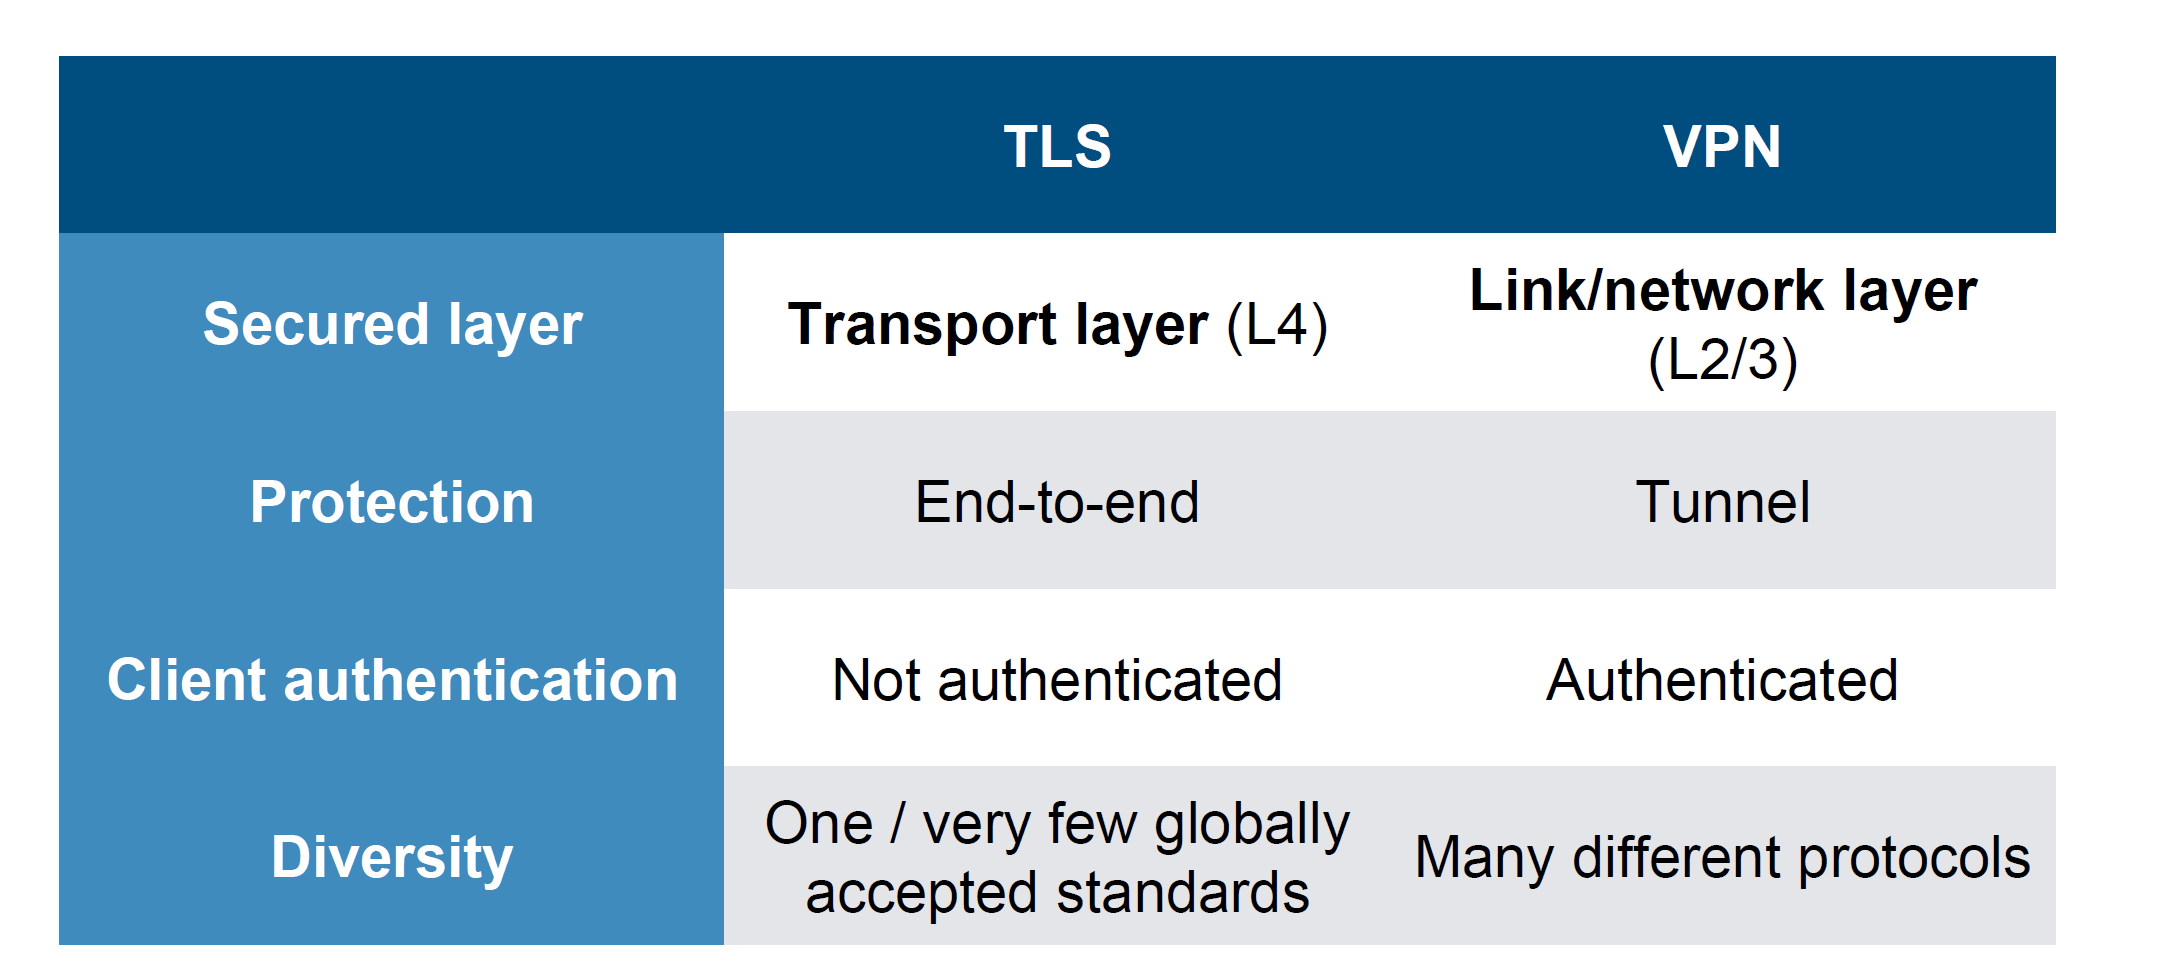
\includegraphics[width=\linewidth]{Figures/VPN_tls.PNG} 
\end{minipage}

\paragraph{Availability/Performance of VPNs:}
\begin{itemize}
    \item VPNs can negatively impact performance (potential detours, limited bandwidth at VPN server, additional crypto)
    \item Generally VPNs do not provide higher availability (no DDoS defence)
    \item VPNs can defend against targeted packet filtering (Routers can recognize VPN packets but not content
\end{itemize}

\paragraph{VPN vs VLAN}
\begin{itemize}
    \item VPN: connects two different networks
    \item VLAN: set up multiple isolated virtual networks on a single physical infrastructure.
\end{itemize}

\textcolor{orange}{Look at schema example of VPN routing on slide 21}

\subsection{IPsec}

\begin{enumerate}
    \item Set up a security association (SA) via IKE
    \item Encapsulate packets and tunnel them between SA endpoints
\end{enumerate}

IPsec is a very large and complicated protocol. The tunnel is setup at layer 3 (network). In IPsec, we also use sequence numbers (like in TLS) \textit{but} they are included in the packets (while TLS doesn't include sequence numbers in the packet). That's because IPsec runs on top of IP and IP is best-effort transport. The ordering of packets can thus be off at the receiver. That's why sequence numbers need to be in the packets. What if we are tunneling UDP traffic?
The numbers are also there to avoid replay attacks. Each party has a sliding window so that it can
detect if a packet is replayed by inspecting the sequence number. IPsec and IKE have many options and modes

\paragraph{Problems with IPsec}
\begin{itemize}
    \item Configuration is difficult and error-prone due to many options.
    \item Some options do not provide any security
\end{itemize}

\subsubsection{Internet key exchange (IKEv2)}

IKE is used to setup a security association (SA). In IKE, we have an anonymous DH exchange. This provides forward security and does not leak identities (as e.g. TLS does) since no authentication data is sent in plaintext. The disadvantage is that anonymous DH is vulnerable to an active MiTM attack.

\begin{minipage}{\linewidth}
    \centering      
    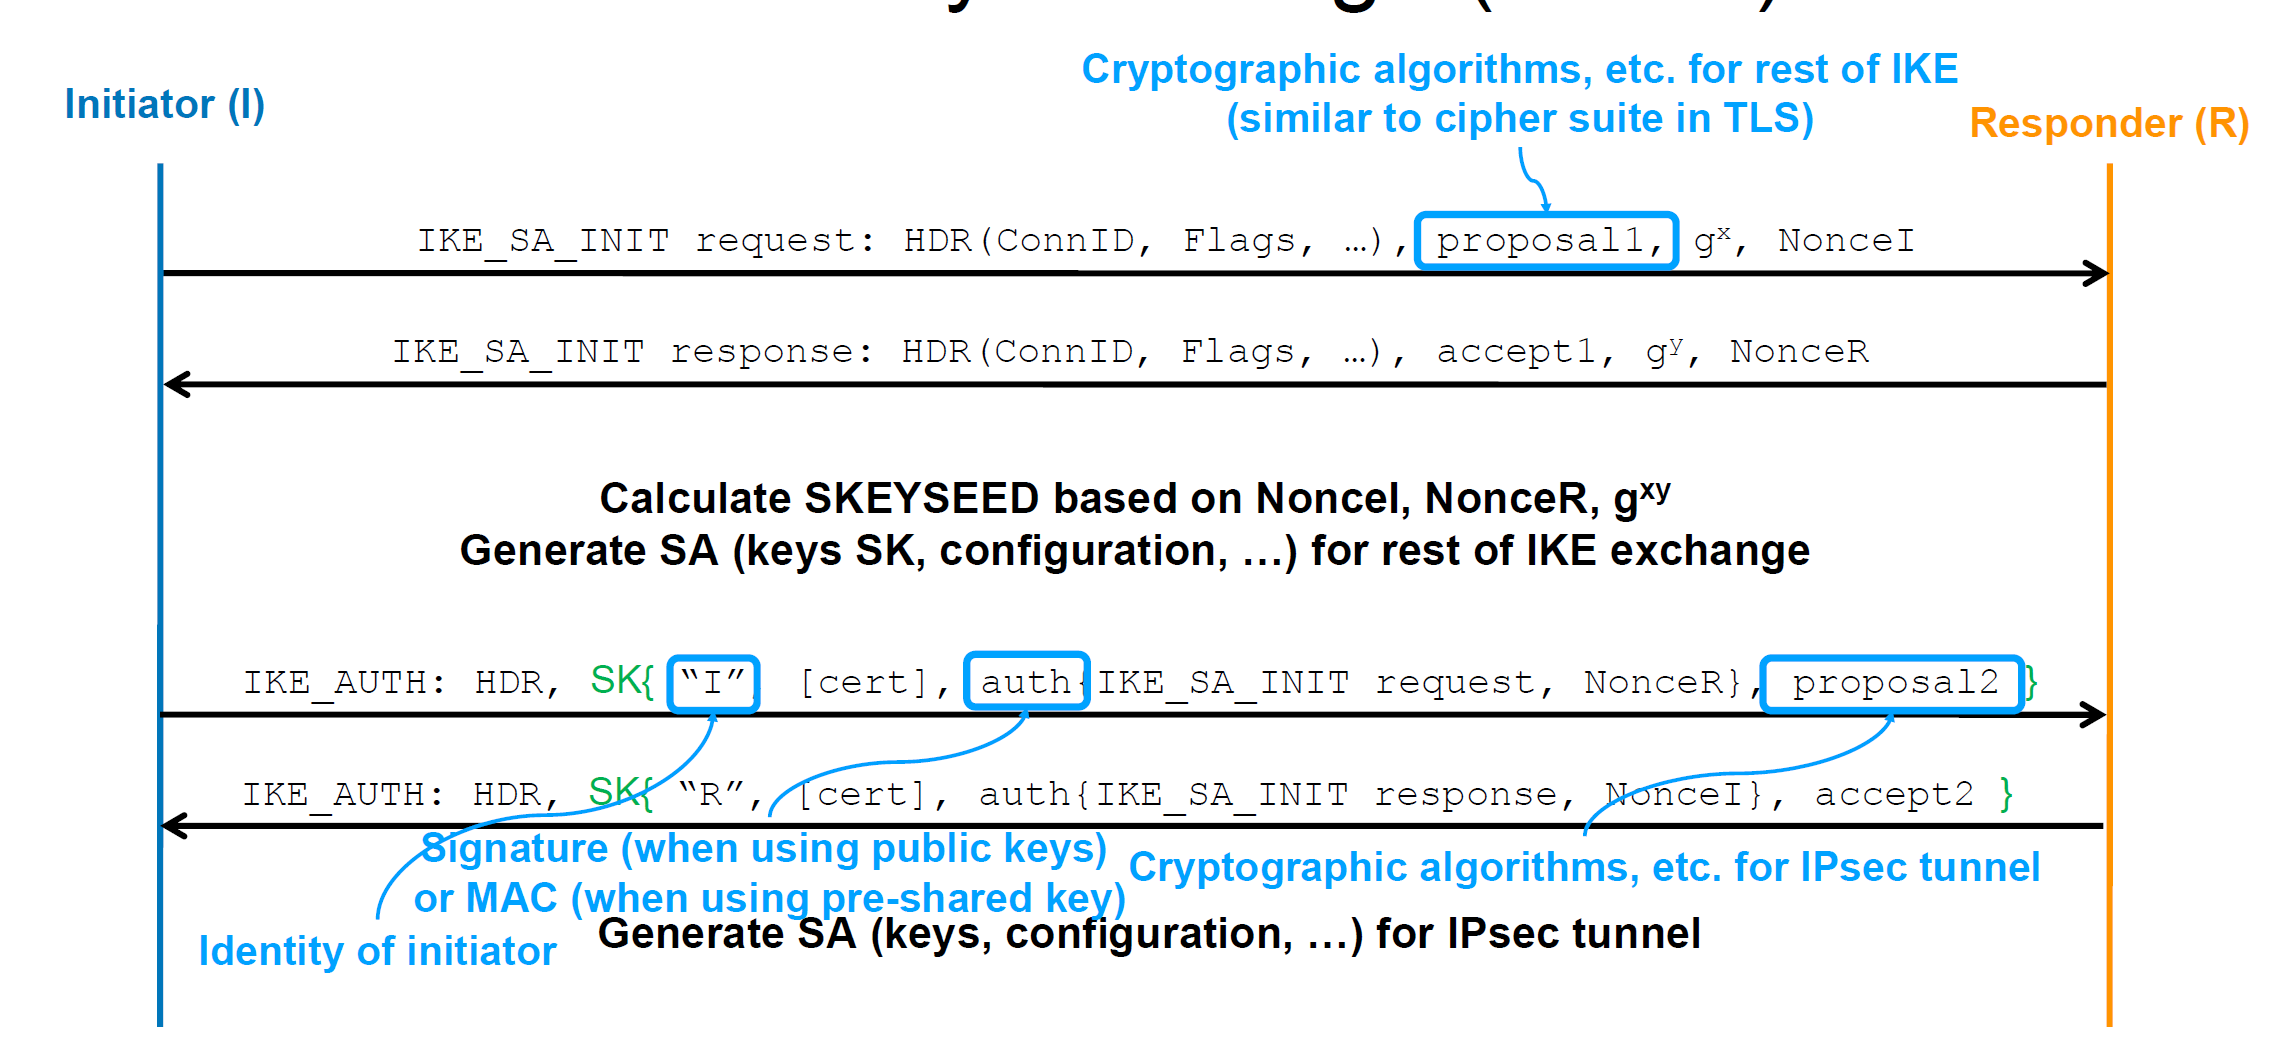
\includegraphics[width=\linewidth]{Figures/VPN_IKE.PNG} 
\end{minipage}

\subsubsection{IPsec session}

After an SA was setup using IKE, we encapsulate packets and tunnel them between SA endpoints. Encapsulation works as follows:

\begin{itemize}
	\item Add ESP trailer: Padding, type encapsulated (original) packet
	\item Encrypt packet and trailer
	\item Add ESP header: SA identification, sequence number
	\item Create Integrity Check Value (ICV): MAC over original packet, ESP	header, ESP trailer
	\item Add new IP header
\end{itemize}

\begin{minipage}{\linewidth}
    \centering      
    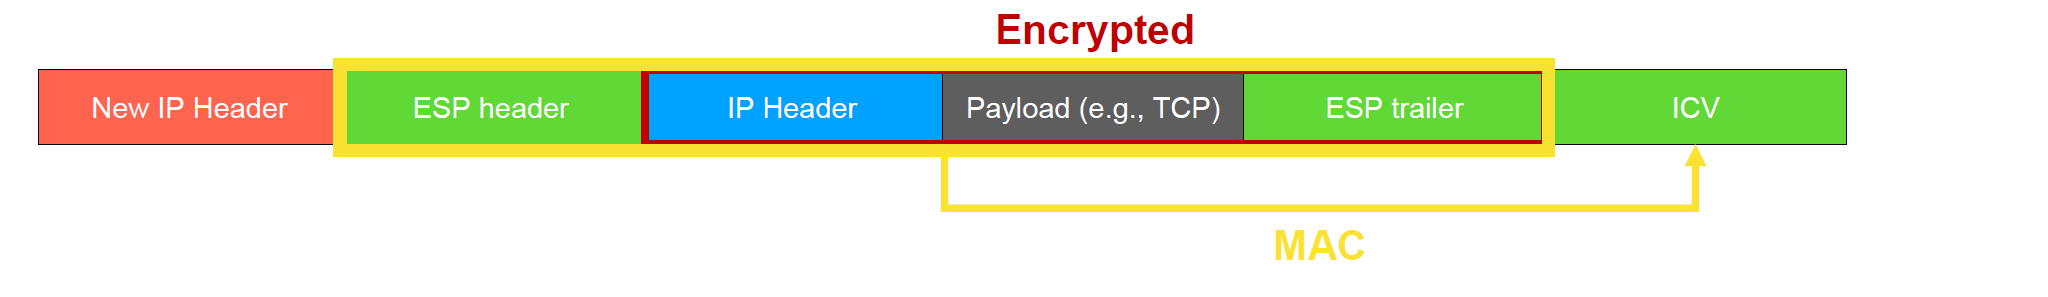
\includegraphics[width=\linewidth]{Figures/VPN_session.PNG} 
\end{minipage}

Similarly, decapsulation:

\begin{itemize}
	\item Strip off outer IP header
	\item Look up keys and configuration using information in ESP header
	\item Check MAC
	\item Strip off authentication tag and ESP header
	\item Decrypt original packet
	\item Remove ESP trailer
	\item Forward original packet
\end{itemize}

\begin{minipage}{\linewidth}
    \centering      
    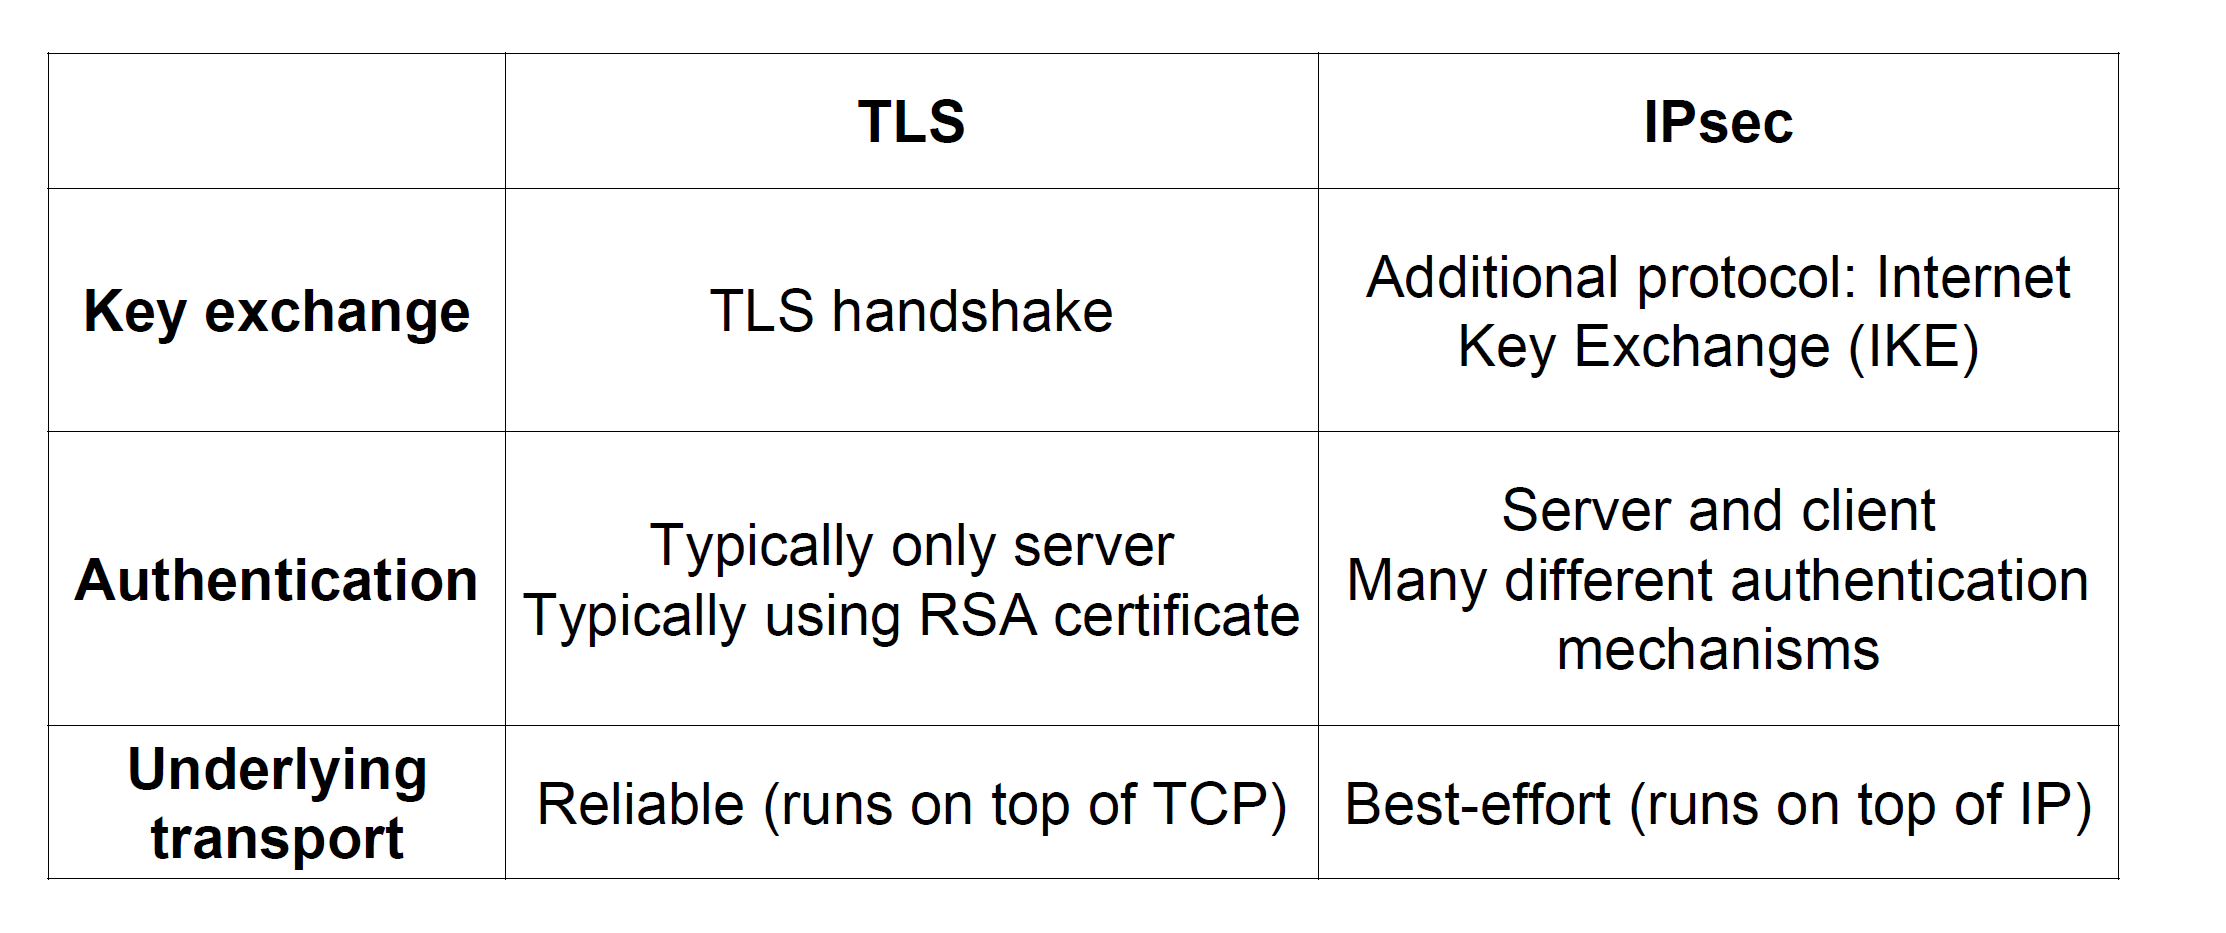
\includegraphics[width=\linewidth]{Figures/VPN_ipsec_tls.PNG} 
\end{minipage}

\subsection{Wireguard}

WireGuard is a modern lightweight VPN that only has roughly 4000 LOC (opposed to OpenVPN with 600'000 LOC!).\\
WireGuard relies on simple configuration and no cryptographic agility. It only uses state-of-the-art primitives: Curve25519 (signatures), ChaCha20 (encryption), Poly1305 (authentication). The small codebase provides minimal attack surface and is formally verifiable. Wireguard is faster than IPsec or OpenVPN. 

\subsubsection{Authentication and keys}

Each peer has a static key pair. Initiator: $S_I^{pub}, S_I^{priv}$, Responder: $S_R^{pub}, S_R^{priv}$. Peers specify in configuration which public keys are authorized. WireGuard uses a 1-RTT handshake during which each peer generates an ephemeral key pair: Initiator: $E_I^{pub}, E_I^{priv}$, Responder: $E_R^{pub}, E_R^{priv}$. Symmetric keys are then derived from four DH combinations: $$\{DH(S_I,S_R), DH(S_I,E_R), DH(E_I,S_R), DH(E_I,E_R)\}$$

\begin{minipage}{\linewidth}
    \centering      
    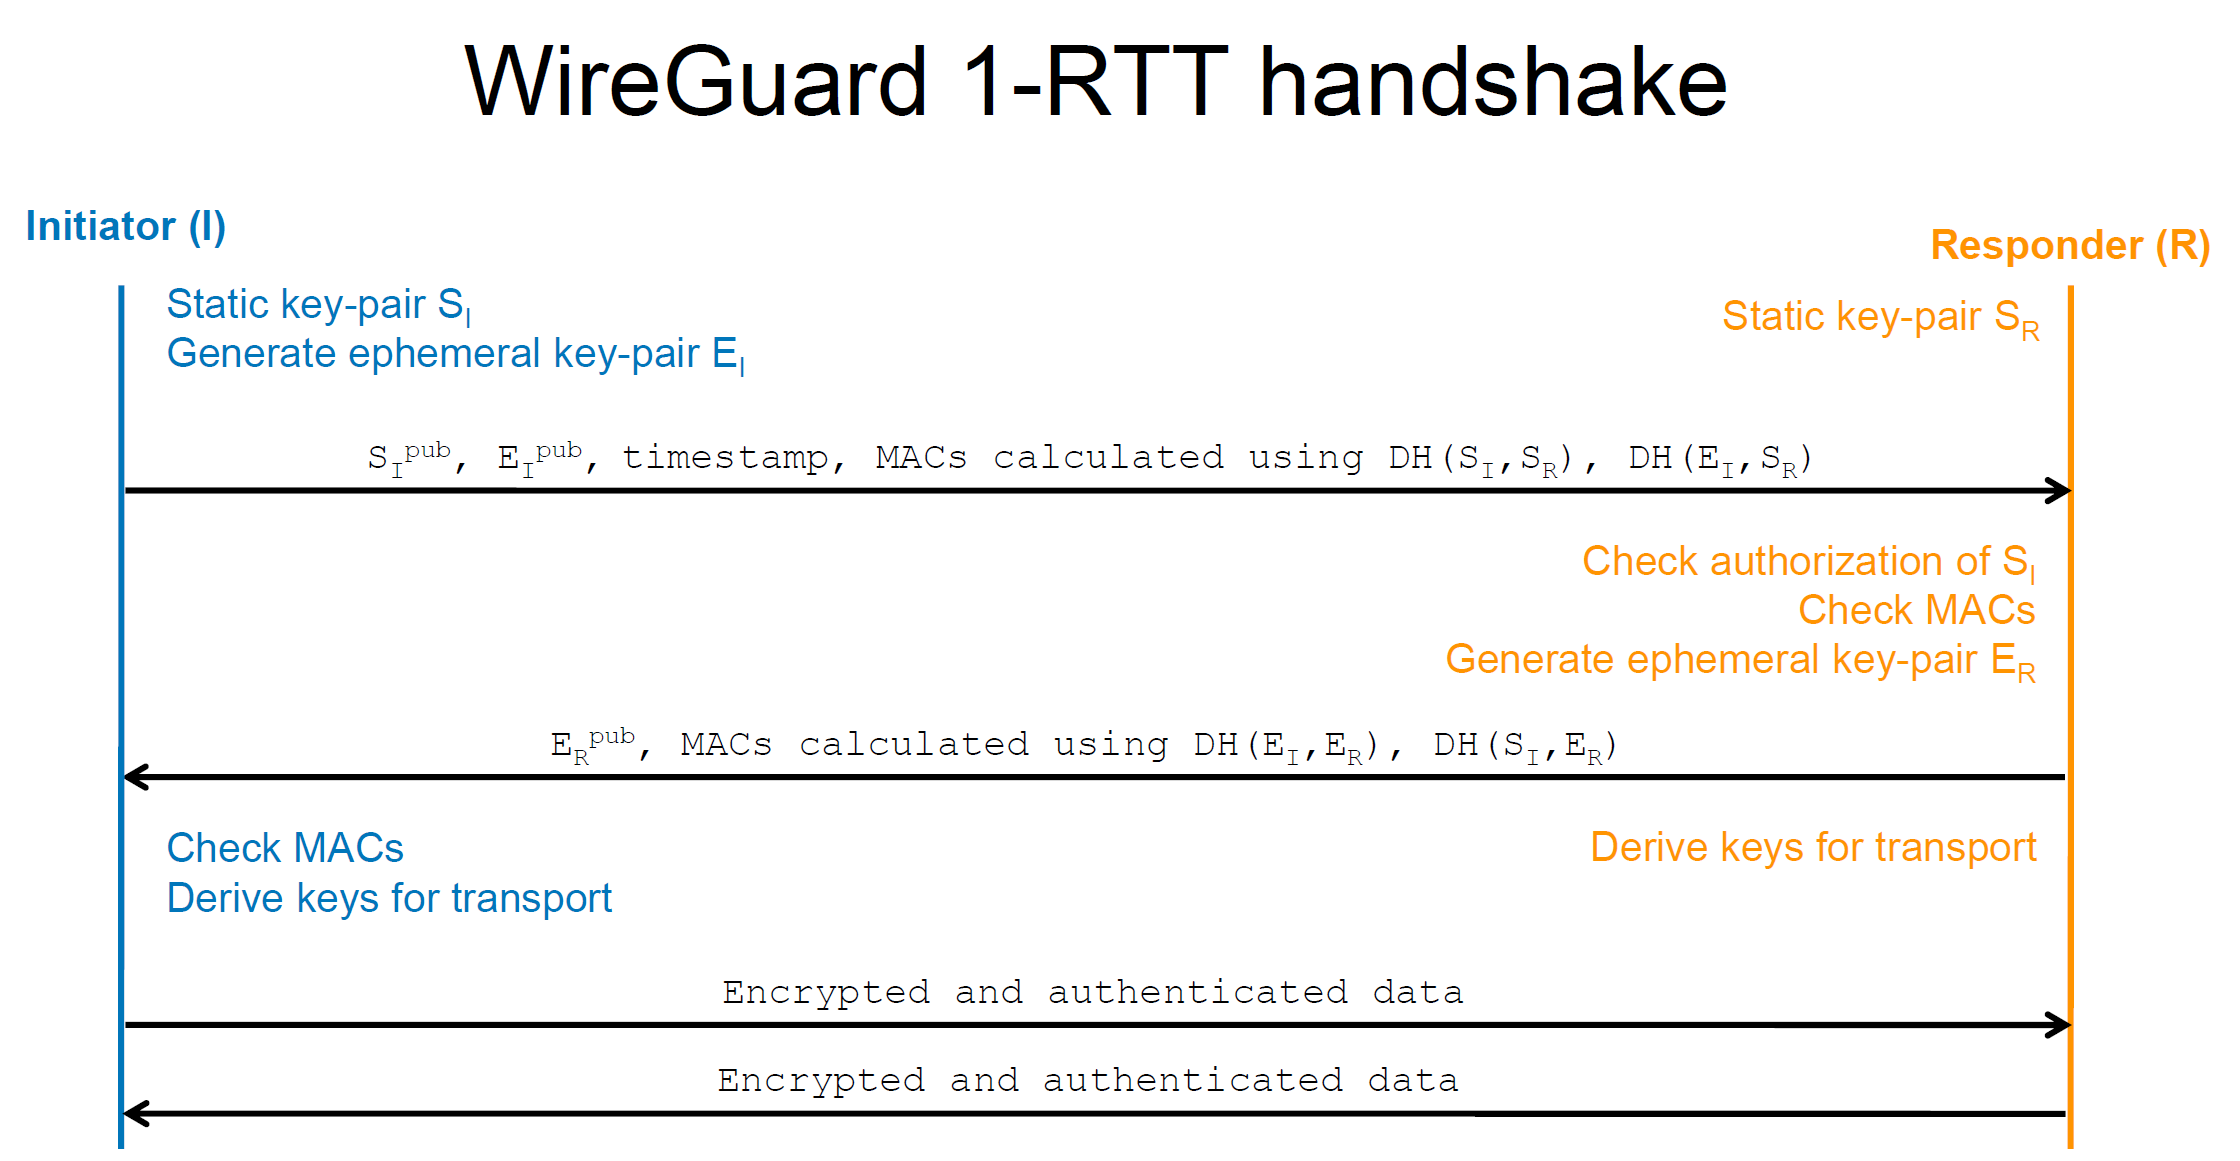
\includegraphics[width=\linewidth]{Figures/VPN_wireguard.PNG} 
\end{minipage}

The WireGuard protocol is connectionless. A series of timers, both based on message counts and time, are used to steer key renegotiation, handshakes and session termination. The strict key rotation timers \texttt{(REKEY\_AFTER\_MESSAGES, REKEY\_AFTER\_TIME)} and the ephemeral
ECDH session key exchange guarantee PFS.

\subsubsection{DoS protection}

Since VPN servers need to do expensive crypto, they are susceptible to (D)DoS attacks. A WireGuard implementation can choose to respond with a cookie instead of processing the handshake: the initiator will then use this cookie as a key for computing HMACs of their message. The cookie mechanism of IKEv2 is very similar to the one just described. However, an important difference between the two is that Wireguard requires an additional MAC on the handshake message — using the public key of the responder as HMAC key. This allows the responder to stay completely silent — not responding even with a cookie — unless the initiator knows its public key. (Remember that “public” key do not need to be publicly accessible, often they are not).



\section{Anonymous communication systems}

Why are VPNs and TLS not enough? VPN server still sees metadata such as srcIP, dstIP, ports, metadata etc. We need something stronger for anonymous communication. TLS does not hide src and dest address.

\subsection{Terminology: “anonymity”}

\begin{itemize}
	\item \textbf{Sender anonymity:} adversary knows/is receiver, may learn message, sender is unknown. The sender anonymity set is the set of all possible senders, which can be used as a (rough) metric. A small set means little anonymity. Return address is a token provided by original sender.
	\item \textbf{Receiver anonymity:} Adversary knows sender, may learn message, receiver is unknown. The sender needs a return address: the receiver provides a token (since the sender doesn't know the receiver) and the token will be used to direct the message. Receiver anonymity set is the set of all possible receivers.
	\item \textbf{(Sender-receiver) unlinkability:} Adversary knows senders, knows receivers, link between senders and	receivers is unknown. Multiple users need to communicate at the same time. Anonymity --> Unlinkability
	\item \textbf{Unobservability:} Adversary cannot tell whether any communication is taking place.
	\item \textbf{Plausible Deniability:} Adversary cannot prove that any particular individual was responsible for a message (or other action). Anonymity --> plausible deniability
\end{itemize}

The following holds: $Unobservability \rightarrow Anonymity \rightarrow Unlinkability$

\paragraph{Threat Model: } 
\begin{itemize}
    \item Degree of control: Local or global
    \item Type of Control: network or compromised infrastructure
    \item Types of Behavior: passive or active
    \item Often quite unspecified attacker model --> unclear guarantees
\end{itemize}

\subsection{Basics of Anonymous Communication}

\paragraph{What Mechanisms can we use?}
\begin{itemize}
    \item \textbf{Broadcast:} Receiver anonymity is guaranteed, sender can be de-anonymized (localization through triangulation)!. 
    \item \textbf{Hijacked Connection:} burner phone, hacked WiFi, network ID != personal sender ID.
    \item \textbf{Proxy or VPN with layered encryption:} Proxy can see metadata (src, dest) 
    \item[-->] \textbf{Cascade of multiple proxies} Each proxy only sees addresses of two neighbors, due to layered encryption. Works as long as message passes one honest proxy. 
    \item[-->] However the attacker may link in and outgoing messages through timing.
\end{itemize}

\subsection{Mixnets}

\paragraph{Batching and Mixing:}
Collect a number of messages before forwarding (Batching), change the order of the messages (Mixing), also we need to padd messages to a fixed length.\\
An adversary can still mount an \textbf{intersection attack:} Often, users only communicate with a
small subset of other users. Every time a message is seen by the target, register the sets of destinations. 

\paragraph{Cover traffic for unobservability:}
To achieve full unobservability, use \textbf{cover traffic}, both for sending and receiving. Now we are fully anonymous, as long as one mix is honest. \\
How do we handle return addresses? Alice prepares a return address and encloses it in her first message. That address contains layered information.


\subsection{Circuit-based systems (AKA onion-routing system)}
Mix-nets are very secure but very slow. We want a system that can support web browsing.\\
Circuit-based anonymous communication systems, commonly known as Onion Routing Systems. The nodes are called relays (also nodes or routers), there are usually 3 of them Entry guard, Middle relay and Exit relay. The virtual circuit is also called tunnel.
\begin{itemize}
    \item Main ideas: use layered encryption, no batching and mixing, no cover traffic.
    \item Flow-based: establish a virtual circuit (keys) once per flow, reuse it for all packets in the flow using only symmetric key crypto.
    \item The threat model is constrained: only a local adversary (e.g. ISP) which cannot launch confirmation attacks.
\end{itemize}

\paragraph{Circuit setup}
\begin{itemize}
    \item Initially, sender knows long-term public keys of relays.
    \item The sender negotiates shared keys with all relays on the path (this requires expensive asymmetric key cryptography)
    \item The relays store the necessary state.
\end{itemize}
\textbf{Direct circuit setup:} a packet is sent through the whole system and returned and at each step the state is generated. The encryption keys of data are only based on public keys of relays. Thus (immediate) Forward Security does not hold since no ephemeral information is used. We can achieve eventual forward security by changing public keys of the relays regularly \\
\textbf{Telescopic circuit setup:} Keys are negotiated one relay at a time. The circuit is “extended” by one hop at a time (that’s why it is called telescopic). Ephemeral session keys are negotiated before the circuit is extended. This setup is slower... but it offers immediate forward secrecy: As soon as the circuit is closed, the session keys are deleted.

\paragraph{Data forwarding}

The sender has established a circuit (keys and per-link IDs). A data packet is encrypted as usual (layered encryption). The ID of the next relay is added in clear text. To protect against network adversaries, links can be encrypted (TLS).

\paragraph{Circuit tear-down}

Can be initiated both by sender and by intermediate relays. The sender communicates the tear-down to one relay at a time, starting from the furthest away. The exit relay may tear down the circuit if a corrupt packet is detected, or some other attack. Circuits have a limited lifetime, so they will eventually be destroyed.

\begin{minipage}{\linewidth}
    \centering      
    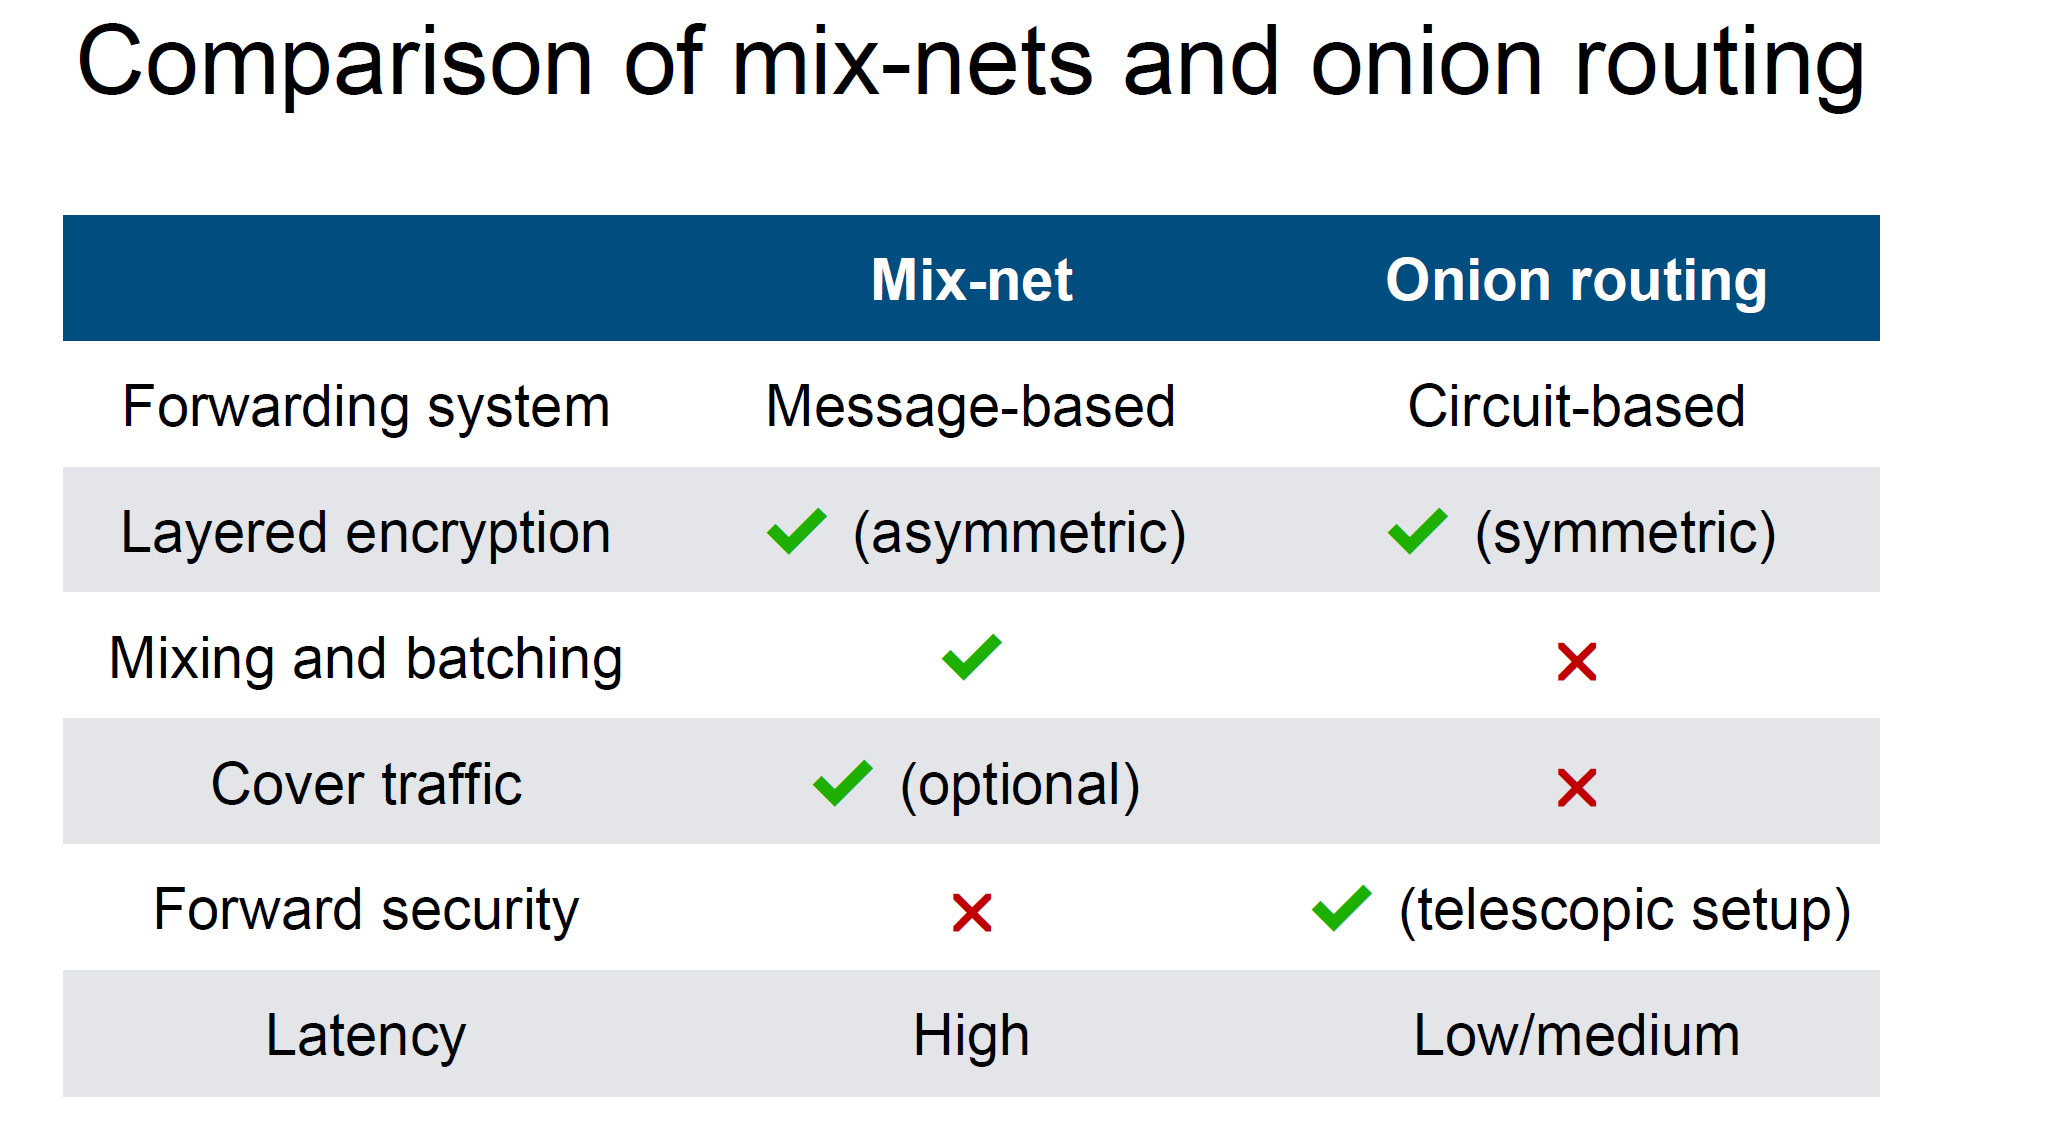
\includegraphics[width=\linewidth]{Figures/Anym_mix_nets.PNG} 
\end{minipage}

\subsection{Attacks on circuit-based anonymous-communication systems}

Many attacks have been proposed, however for many it is unclear if they fit the standard threat model. Some of them are practical, requiring limited resources. Others are only achievable by state-level adversaries (Five Eyes).

\paragraph{Traffic Analysis:}
\begin{itemize}
	\item Passive traffic analysis: The adversary observes the edges of the network, recording traffic patterns. Real-time detection is challenging, alternative is store and compare later.
	\item Active traffic analysis: 
	\begin{itemize}
		\item The adversary actively modifies packet timings: Inter-packet timings (delaying/reordering packets), packet drops also possible but detectable
		\item Flow watermarking: inject one bit of information (marked or not)
		\item Flow fingerprinting: inject multiple bits (e.g., sender IP address!)
	\end{itemize}
	\item Website fingerprinting: Many websites have a distinct pattern of traffic they receive and send. Adversary can keep a database of patterns and compare traffic recorded from a single observation point (ISP, WiFi users,...)
\end{itemize}

\paragraph{Denfence against Traffic Analysis:}
\begin{itemize}
    \item Cover traffic and mixing: significant overhead, scalability becomes an issue. Only suitable for few applications (VoIP) with low bandwidth.
\end{itemize}

In order to prevent traffic analysis, you should omit \textit{everything} that makes you stand out: don't install any plugins, never use TOR in fullscreen mode (gives away your screen resolution), don't type inside the browser, type inside a text-editor and copy-paste messages into webforms, etc.

\subsubsection{Higher-layer attacks}
\begin{itemize}
	\item OS Network stack fingerprinting: Compromised adversary can probe TCP stack, solution would be per-hop TCP. Still TLS or HTTP layer may be identifiable.
	\item Most deanonymization is still done through other means: Trick user into downloading malware, trick user into downloading file that will access the Internet directly, analyze user behavior like texts.
\end{itemize}

To achieve anonymity, all layers need to be anonymized: Any gap will break anonymity!

\subsection{Tor}

\paragraph{Tor basics:}
\begin{itemize}
	\item Circuits established over 3 relays
	\item Telescopic setup (forward secrecy!)
	\item Per-hop TCP, established on the fly to avoid TCP stack fingerprinting
	\item Per-hop TLS (except on the last hop). Multiple circuits over same TLS connection. End-to-end HTTPS is possible.
	\item Main tool: Tor browser (Firefox)
\end{itemize}

\paragraph{Tor additional features:}

\begin{itemize}
	\item Exit policies (exit can restrict the destinations	they connect to)
	\item Multiple streams per circuit (helps with performance, weakens anonymity)
	\item Censorship resistance (bridges)
	\item Hidden services: Provide receiver anonymity, use .onion URL (not in DNS). The name is the hash of the HS’s public key.
\end{itemize}

\subsubsection{Cells}

Basic unit in Tor. If a relay obtains a cell: it looks up keying material from circuit id and will decrypt the payload which contains sets of fields. The relay then checks the digest and if it matches it looks at the cmd.

\begin{minipage}{\linewidth}
    \centering      
    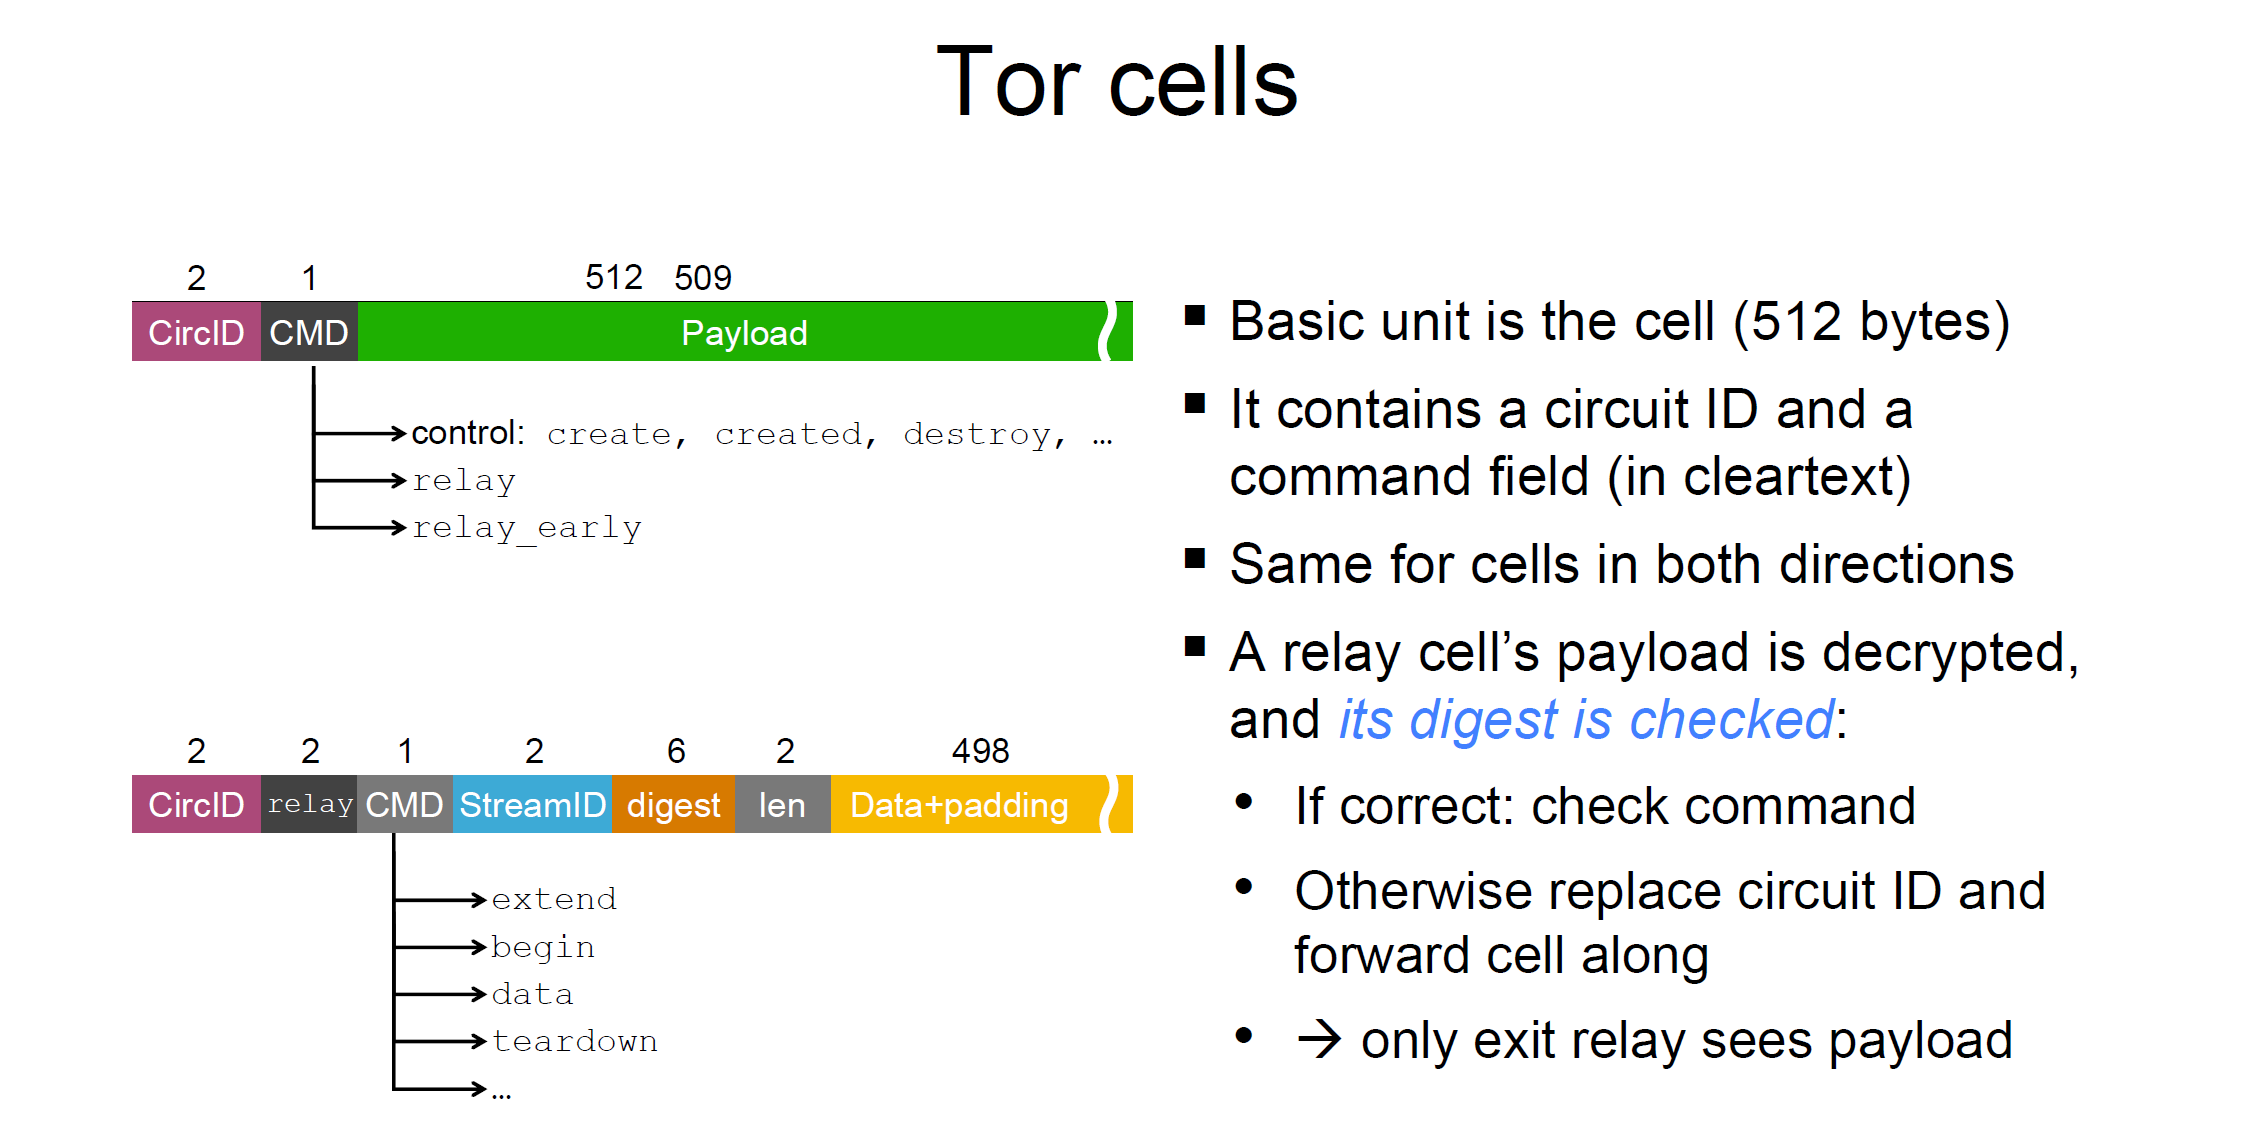
\includegraphics[width=\linewidth]{Figures/Anym_tor_cell.PNG} 
\end{minipage}

\paragraph{Circuit extension with relay\_early:}
\begin{itemize}
    \item Path of arbitrary length can be used for very cheap DoS: Simply create a circuit that goes through all honest nodes, dozens of times: incredibly large amplification factor.
    \item Solution: Tor extend cells can only be contained in relay early cells
\end{itemize}
\\
\textbf{Hidden Services:}\\
\begin{minipage}{\linewidth}
    \centering      
    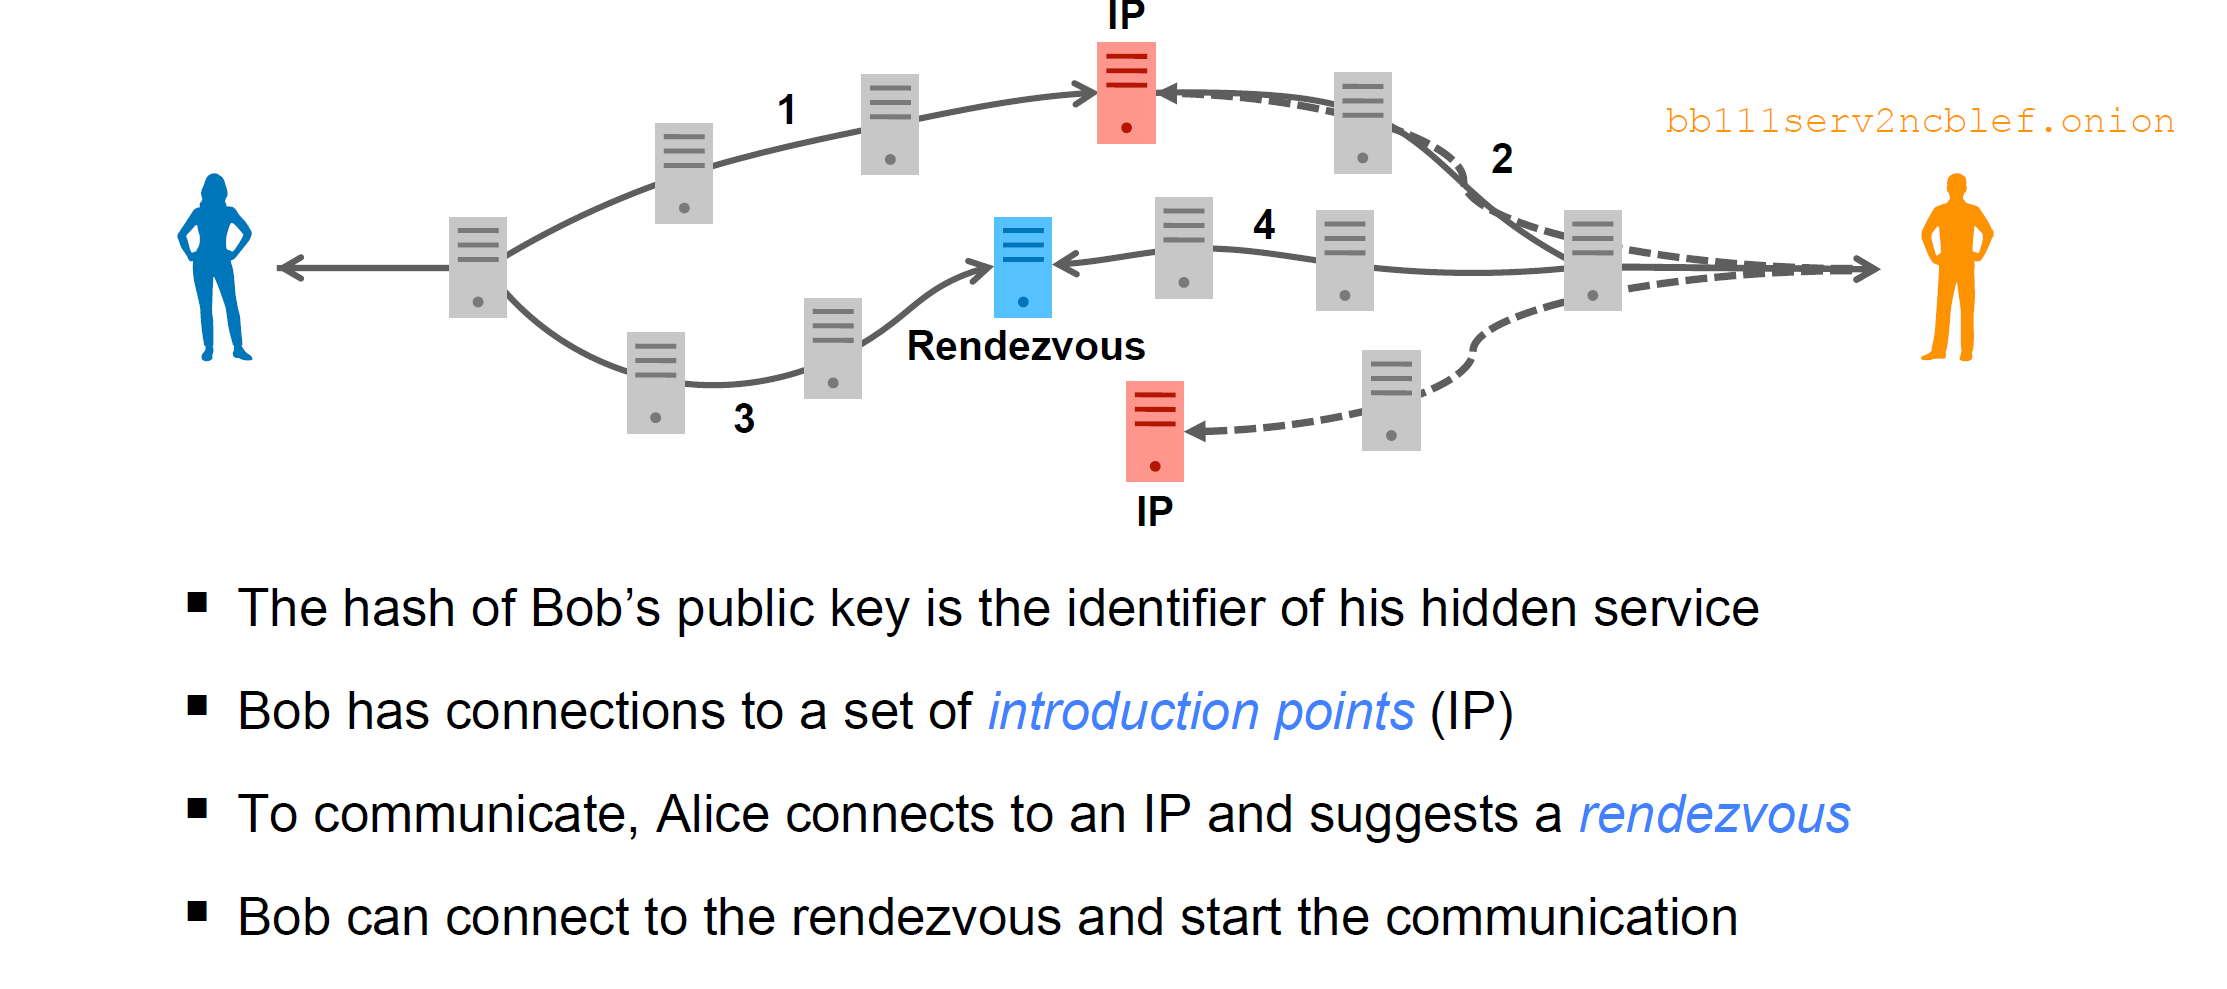
\includegraphics[width=\linewidth]{Figures/Anym_hidden_services.PNG} 
\end{minipage}

\subsubsection{Directory authorities}

\begin{itemize}
    \item How do the clients know what relays there are? 10 directory authorities (servers) running a consensus algorithm.
    \item The authorities track the state of relays, store their public keys.
    \item Client software (Tor browser) comes with a list of the authorities’ keys (If an adversary can supply the list, de-anonymization is trivial!). A client accepts a consensus document if signed by $\geq$ 50\%.
    \item The centralized authorities are an important weakness of Tor. An adversary compromising 5 authorities can compromise Tor.
    \item Every relay periodically reports a signed statement (state, stats.) 
    \item DAs also act as bandwidth authorities: verify bandwidth of nodes.
    \item Sybil protection: DAs limit the number of relays per IP subnet
\end{itemize} 

\subsubsection{Censorship resistance in Tor}
\begin{itemize}
    \item Problem: relay nodes are publicly listed and can be blocked.
    \item The Tor network contains a number of bridge relays (or bridges). Not (all) publicly listed, instead distributed through friends networks. This is used to circumvent censors which black-list Tor relays.
    \item Problem: deep packet inspection allows detection of Tor traffic
    \item Solution: obfuscate the traffic (pluggable transports)
\end{itemize}

\subsubsection{Circuit setup}

Who is authenticated on the first hop? Alice is \textit{not}. The entry guard is since Alice encrypted her ephemeral DH value $g^{x_1}$ with the entry guard's pubKey. The entry guard then sends back $g^{y_1}$ and a hash of $g^{x_1y_1}$ which it can only do if it was able to decrypt $g^{x_1}$ which it can only do if it has the privKey.
\begin{figure}[hb]
	\centering
	\includegraphics[width=0.9\linewidth]{figures/tor_circuit_setup}
	\caption{Circuit setup with three hops}
	\label{fig:torcircuitsetup}
\end{figure}
\section{Border Gateway Protocol (BGP) Security}

Why should we care about BGP security when we have secure connections (TLS, VPN, DNSSEC, etc.)? The one that controls BGP controls routing.

\begin{itemize}
	\item Obtain fake TLS certs: use BGP route hijacking in combination with automatic certificate issuance (ACME) to obtain fake TLS certs. BGP allows to reroute HTTP challenge traffic from CA to illegitimate IP.
	\item deanonymize TOR users: reroute TOR exit node traffic and use it for correlation attacks.
	\item hijack DNS requests: hijack routes to DNS servers (e.g. MyEtherwallet hack)
	\item Not all traffic is enrypted/authenticated: DNS, HTTP
	\item Even encrypted traffic leaks timing information (fingerprinting)
\end{itemize}

The problem with BGP is that endusers can't protect themselves. Solving these issues is only possible with ISP cooperation.

\subsection{IP Addresses, Autonomous Systems \& the Border Gateway Protocol}

\textbf{IP addresses:} are globally assigned by ICANN (global authority). ICANN assigns certain IP regions to certain parts of the world. Regional Internet Registries (RIRs) are then responsible to further assign IPs. As of 25th November 2019 15:35 UTC+1, we have officially run out of IPv4 addresses.\\
IP addresses are assigned in prefixes (e.g. /16 prefix has $2^{32-16} - 2= 65534)$ IPs).\\

\textbf{Internet:} The Internet is a network of networks (autonomous systems). Autonomous systems can be ISPs (e.g. DT, Swisscom), global backbone network (e.g. Verizon), universities and large companies (e.g. ETH, Google).\\

\textbf{BGP:} BGP "glues" the internet together: routing protocol between ASes, disseminates information about location and paths for IP prefixes. BGP is a path-vector protocol and follows typical business relationships.\\
BGP speaker sends and receives messages from peers over TCP connections on port 179. Messages sent include: \texttt{OPEN, UPDATE, KEEPALIVE, NOTIFICATION}. Route information is disseminated through \texttt{UPDATE} message using attributes: \texttt{Withdraw, path attributes, network layer reachability information}.\\
\\
\paragraph{BGP Policies: }ASes have different business relationships with each other: provider, peer, customer. Each AS implements peering policies. These decide routes are accepted and advertised based on policies. Policies are configured in the BGP daemons of the AS. Policies can be used to implement filters to prevent route leaks (= falsely announced prefixes), or for business reasons.

\begin{itemize}
	\item Input policy: which paths to keep/ discard
	\item Export policy: which paths do I advertise to neighbors
\end{itemize}

\paragraph{How to create your own ISP:}
\begin{enumerate}
    \item Register an autonomous system number to be able to connect via BGP to other networks
    \item Request Internet number resources from your regional network coordination center (get assigned IPv4 and IPv6 prefixes which can be announced over BGP)
    \item Find other networks to connect to and exchange traffic with
    \item Deploy hardware to the peering location an announce IP prefixes
\end{enumerate}

\subsection{BGP Hijacking}
\textbf{BGP vs. OSPF:} BGP is used as an inter Autonomous System protocol, while OSPF is used to establish routes inside an AS. Also, OSPF is a link-state protocol: routers exchange what they know about the network until all routers have a complete map of the network; then the routers compute the routing tables independently. In BGP, we have a path-vector mechanism: every AS announces the prefixes it owns and all the paths that go through it to neighboring ASes.

\begin{minipage}{\linewidth}
    \centering      
    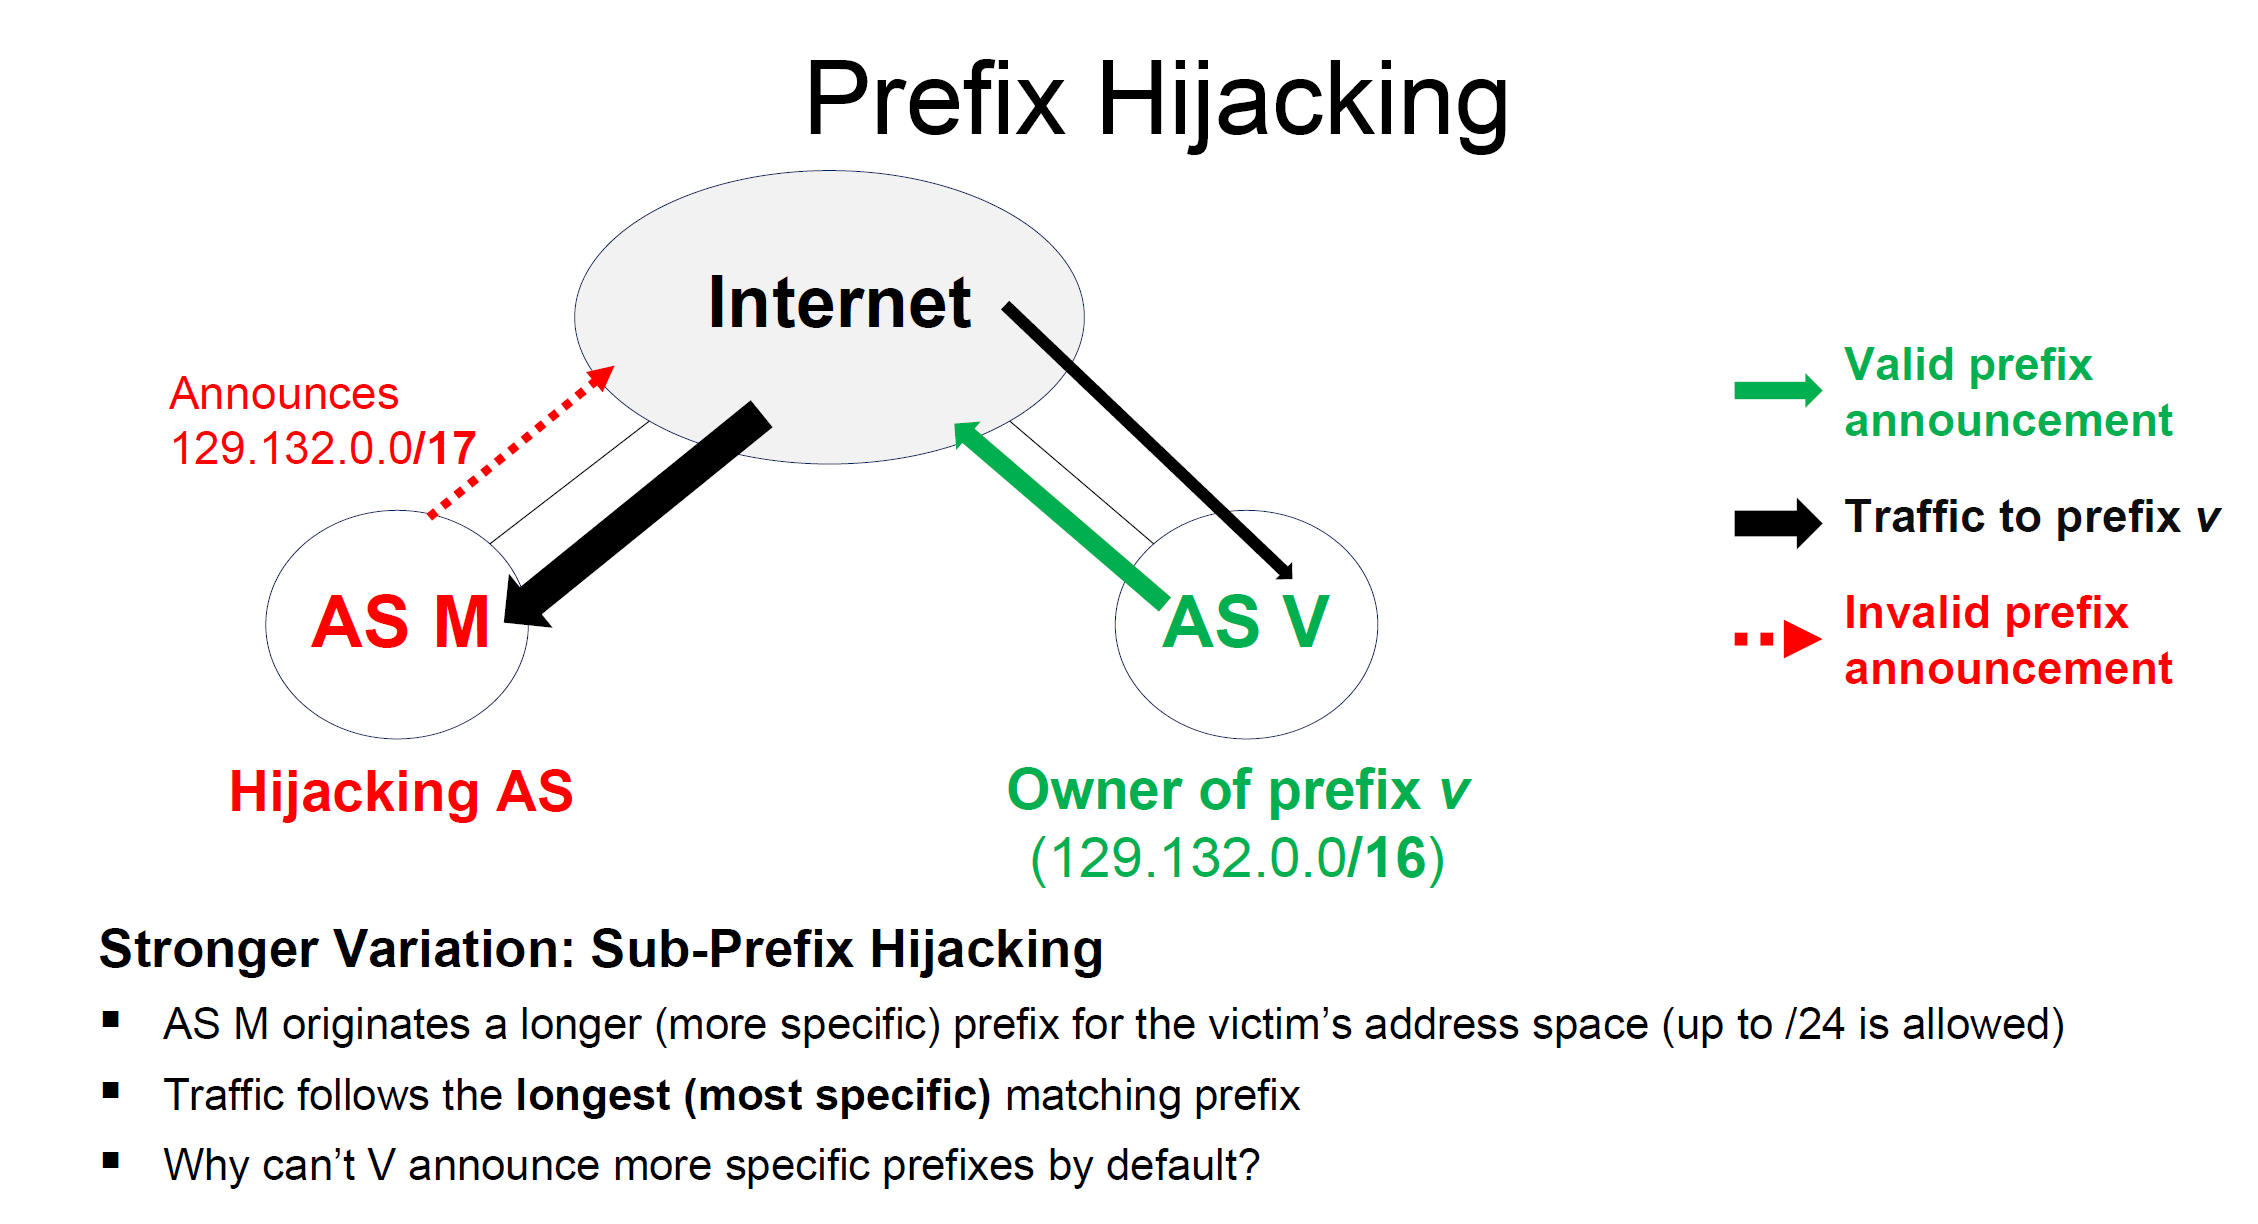
\includegraphics[width=\linewidth]{Figures/BGP_prefix_highjacking.PNG} 
\end{minipage}

Also a less strong attack could be done, where attacker announces same size prefix and only a fraction of traffic to prefix is hijacked. Number of affected sources depends on business relationships, topology, policies.

\subsubsection{Problem 1: BGP does not validate the origin of advertisements!}

\paragraph{IP prefix origination into BGP:} Prefix advertised by the AS who owns the prefix or by upstream providers on its behalf.

\paragraph{IP prefix hijacking:} A malicious or misconfigured AS originates a prefix it does not own, as there is no proper verification in place.

\paragraph{How to perform BGP interception:}
\begin{itemize}
	\item Selective announcement of hijacked prefix only to some neighbors (problem: neighbors may still learn hijacked routes from their peers)
	\item Use BGP poisoning, only select neighbors that use hijacked route.
	\item Use BGP communities to explicitly state to which ASes a particular advertisement should be advertised. Can tell an AS not to forward announcement to specific other ASes using the NoExportSelect action.
\end{itemize}

\paragraph{BGP hijacking in 3 steps:}
\begin{enumerate}
    \item Set up an AS and border router or compromise someone else's router.
    \item Configure router to originate the target (sub-)prefix
    \item Get other ASes to accept the wrong route (Many ASes do not discard wrong routes)
\end{enumerate}
BGP hijacking is not as easy as it sounds (you can't just announce route from your home router). You need access to a BGP router (your own AS or compromised AS).

\subsubsection{Problem 2: BGP does not validate the content of	advertisements}

After a BGP message has been announced, the content of the advertisement is not validated! ASes that receive the advertisement can modify it!

\textbf{ASes can modify the BGP path:}
\begin{itemize}
	\item Remove ASes from the AS path:\\
	Legitimate AS Path: [AS 701, AS 6939, AS 88]. Remove AS 6939: [AS 701, AS 88]\\
	\textbf{Motivation:}
	\begin{itemize}
		\item 	Attract traffic by making path look shorter, attract sources that try to avoid\\
		AS 6939.
	\end{itemize}
	Only AS 701 can tell that the AS path is wrong!
	\item Add ASes to the AS path:\\
	Legitimate AS Path: [AS 701, AS 88]. Add 6939 in-between: [AS 701, AS 6939, AS 88]\\
	\textbf{Motivation:}
	\begin{itemize} 
		\item Trigger loop detection in AS 6939 (AS sees itself on the AS path and drops the advertisement to avoid routing loops) $\rightarrow$ DoS attack on AS 6939, "BGP poisoning".
		\item Make your AS look like it has richer connectivity
	\end{itemize}
	AS 701 can detect the AS path is wrong (but may not care), AS 6939 could detect but may not see the route.
\end{itemize}

\subsection{Attacks on BGP: Obtaining fake certificates}

When using ACME (Automated Certificate Management Environment), a domain is validated through either a HTTP challenge or a DNS challenge to prove that you actually own the domain. By using BGP hijacking, an attacker can:

\begin{minipage}{\linewidth}
    \centering      
    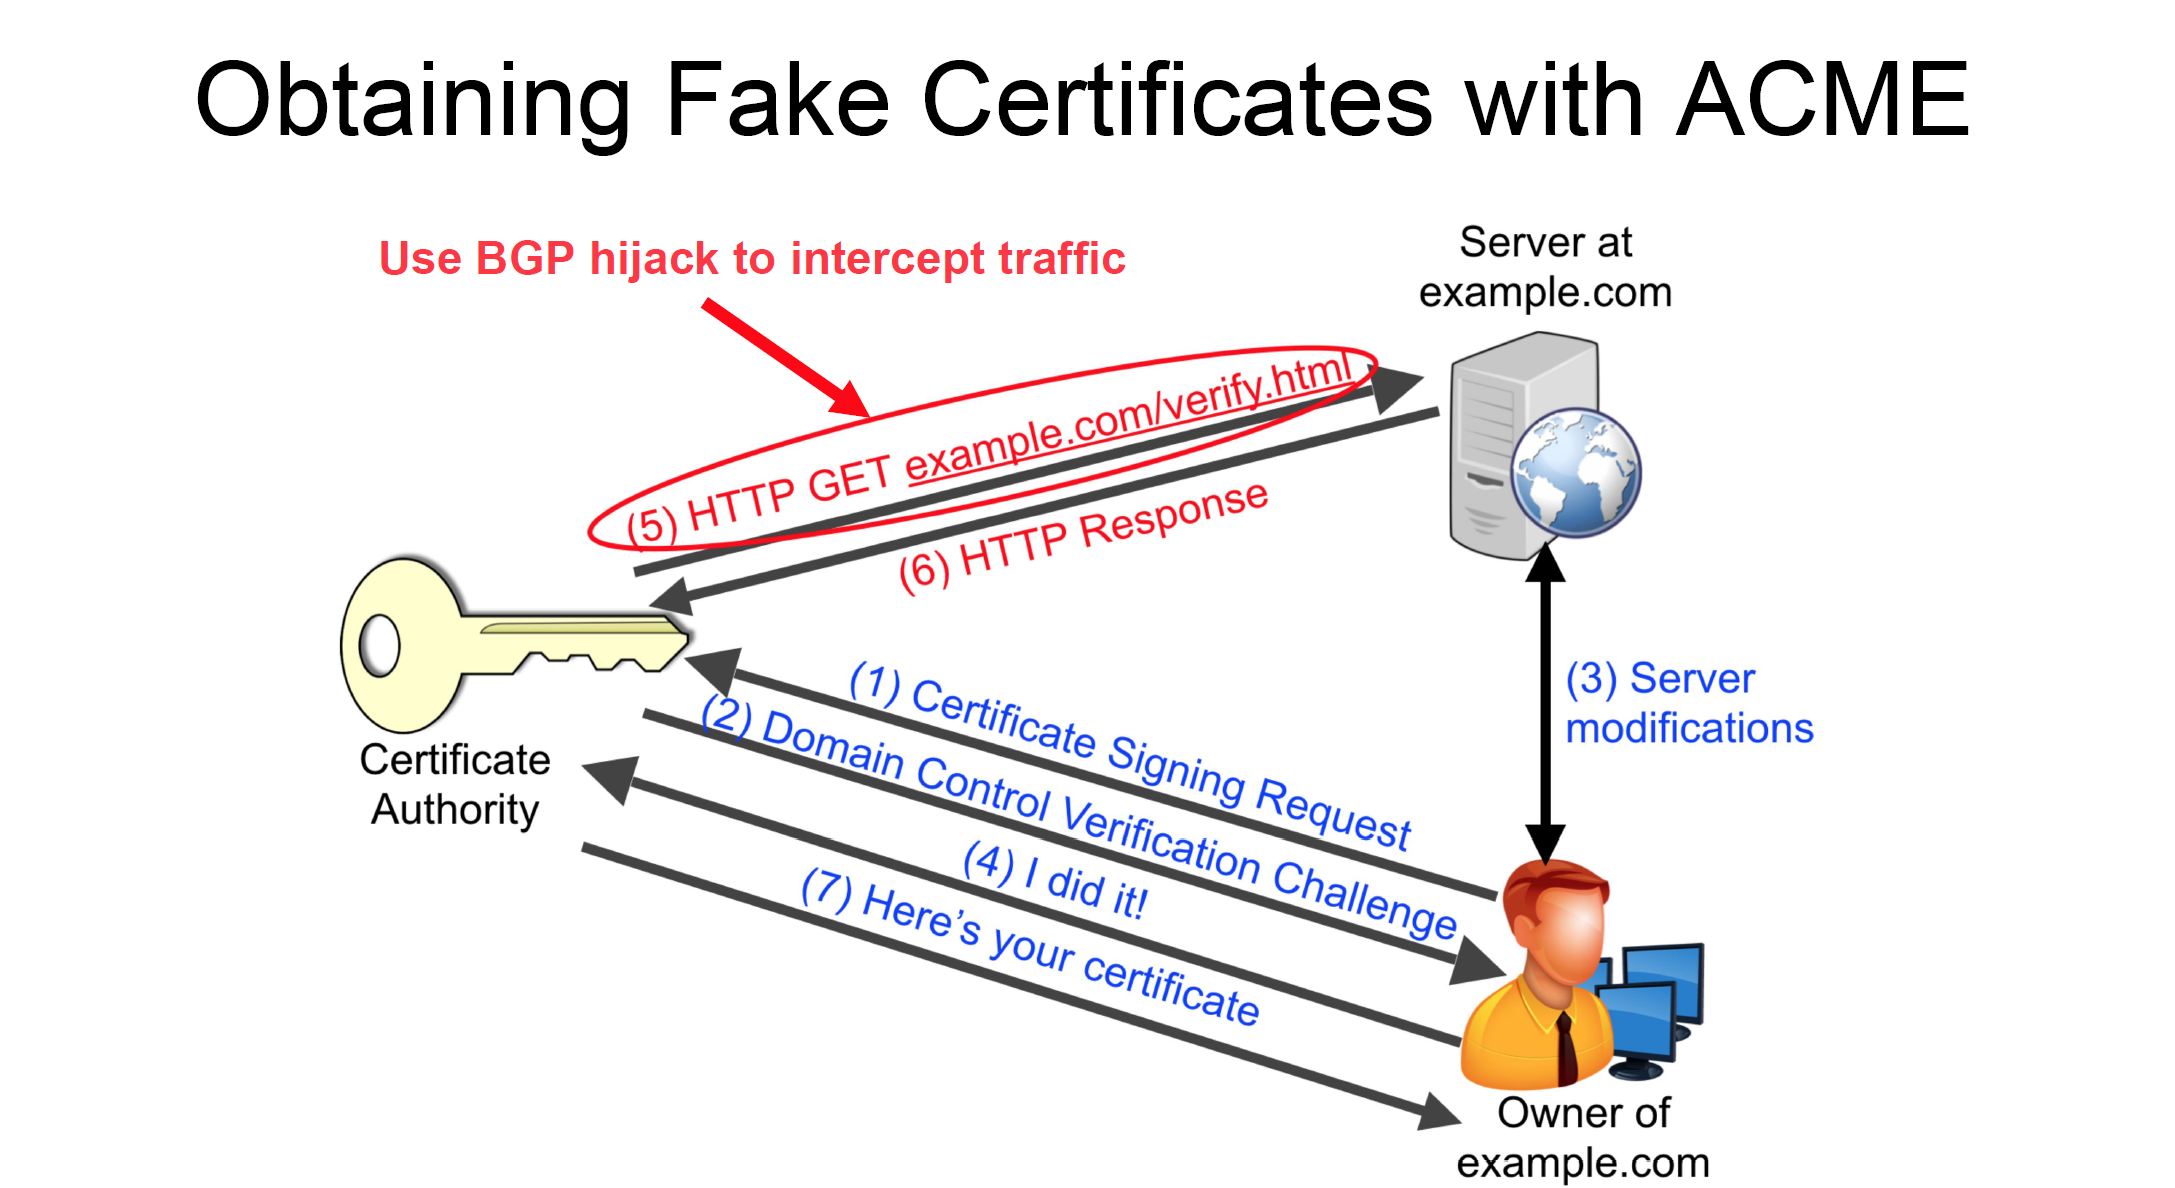
\includegraphics[width=\linewidth]{Figures/BGP_fake_certificates.PNG} 
\end{minipage}

\begin{itemize}
	\item hijack the DNS request of the CA $\rightarrow$ the CA will get a wrong IP owned by the attacker.
	\item hijack the connection to the correct IP and route it to an IP she owns.
\end{itemize}

\subsection{Other attacks on BGP}

\begin{itemize}
	\item Denial-of-service attacks: overload links between BGP routers, send bogus TCP packets (FIN/RST to close session, TCP SYN flood)\\
	A possible solution to bogus TCP RST is to only accept TCP RST with TTL=255, i.e. only TCP RST from direct neighbor router.
	\item Eavesdrop or tamper messages by tapping the link
	\item Most such attacks are easy to defend against and are no longer a large concern
\end{itemize}

\subsection{Countermeasures}
\paragraph{What properties do we want?}
\begin{enumerate}
    \item Only an AS that owns an IP prefix is allowed to announce it (can be proven cryptographically)
    \item Routing messages are authenticated by all ASes on the path (AS cannot add or remove other ASes in BGP announcements)
\end{enumerate}

\subsubsection{Best Current Practices (BCPs)}

\begin{itemize}
	\item Securing the BGP peering session between routers (authentication, prioritize BGP traffic)
	\item Filtering routes by prefix and AS path
	\item Filters to block unexpected control traffic (e.g. ignore TCP RST for BGP if it comes from the inside, implement TTL=255 policy)
	\item Enter prefixes into Internet Routing Registries (IRRs) and filter based on these entries
\end{itemize}

None of these actually have strong security properties (no crypto).

\subsubsection{Solution to Problem 1: Origin Authentication (OA)}
\begin{itemize}
    \item Required: Ability to prove ownership of resources.
    \item Resource Public-Key Infrastructure (RPKI): A secure database to map Internet number resources to a trust anchor. A digital certificate proves that an AS is the current holder of a specific resource. Each regional Internet registry (RIR) is a root of trust.
    \item Enables issuance of Route Origination Authorizations (ROAs): States which AS is authorized to announce certain IP prefixes. Can determine the max length of the prefix that the AS is allowed to advertise (avoid sub-prefix hijacking). Certificate follow same delegation as IP addresses from RIRs
    \item Requires no actual modification to BGP (out-of-band checking)
    \item Trusted local caches collect information from RPKI servers and whitelists are periodically pushed to routers: the verification of signatures is therefore performed offline.
\end{itemize}

If AS M now tries to hijack AS V's prefix $v$, routers will check against ROAs in RPKI for prefix $v$ and see that the announcement is invalid and thus drop it.\\
\textbf{However OA is not enough:} AS M can announce that it has a path to AS V by appending itself on the path \textit{after} the entry for AS V. BGP routers in other ASes check against ROAs in RPKI for prefix $v$, and find a valid ROA for prefix $v$. AS M manages to attract a fraction of traffic for AS V.

\begin{minipage}{\linewidth}
    \centering      
    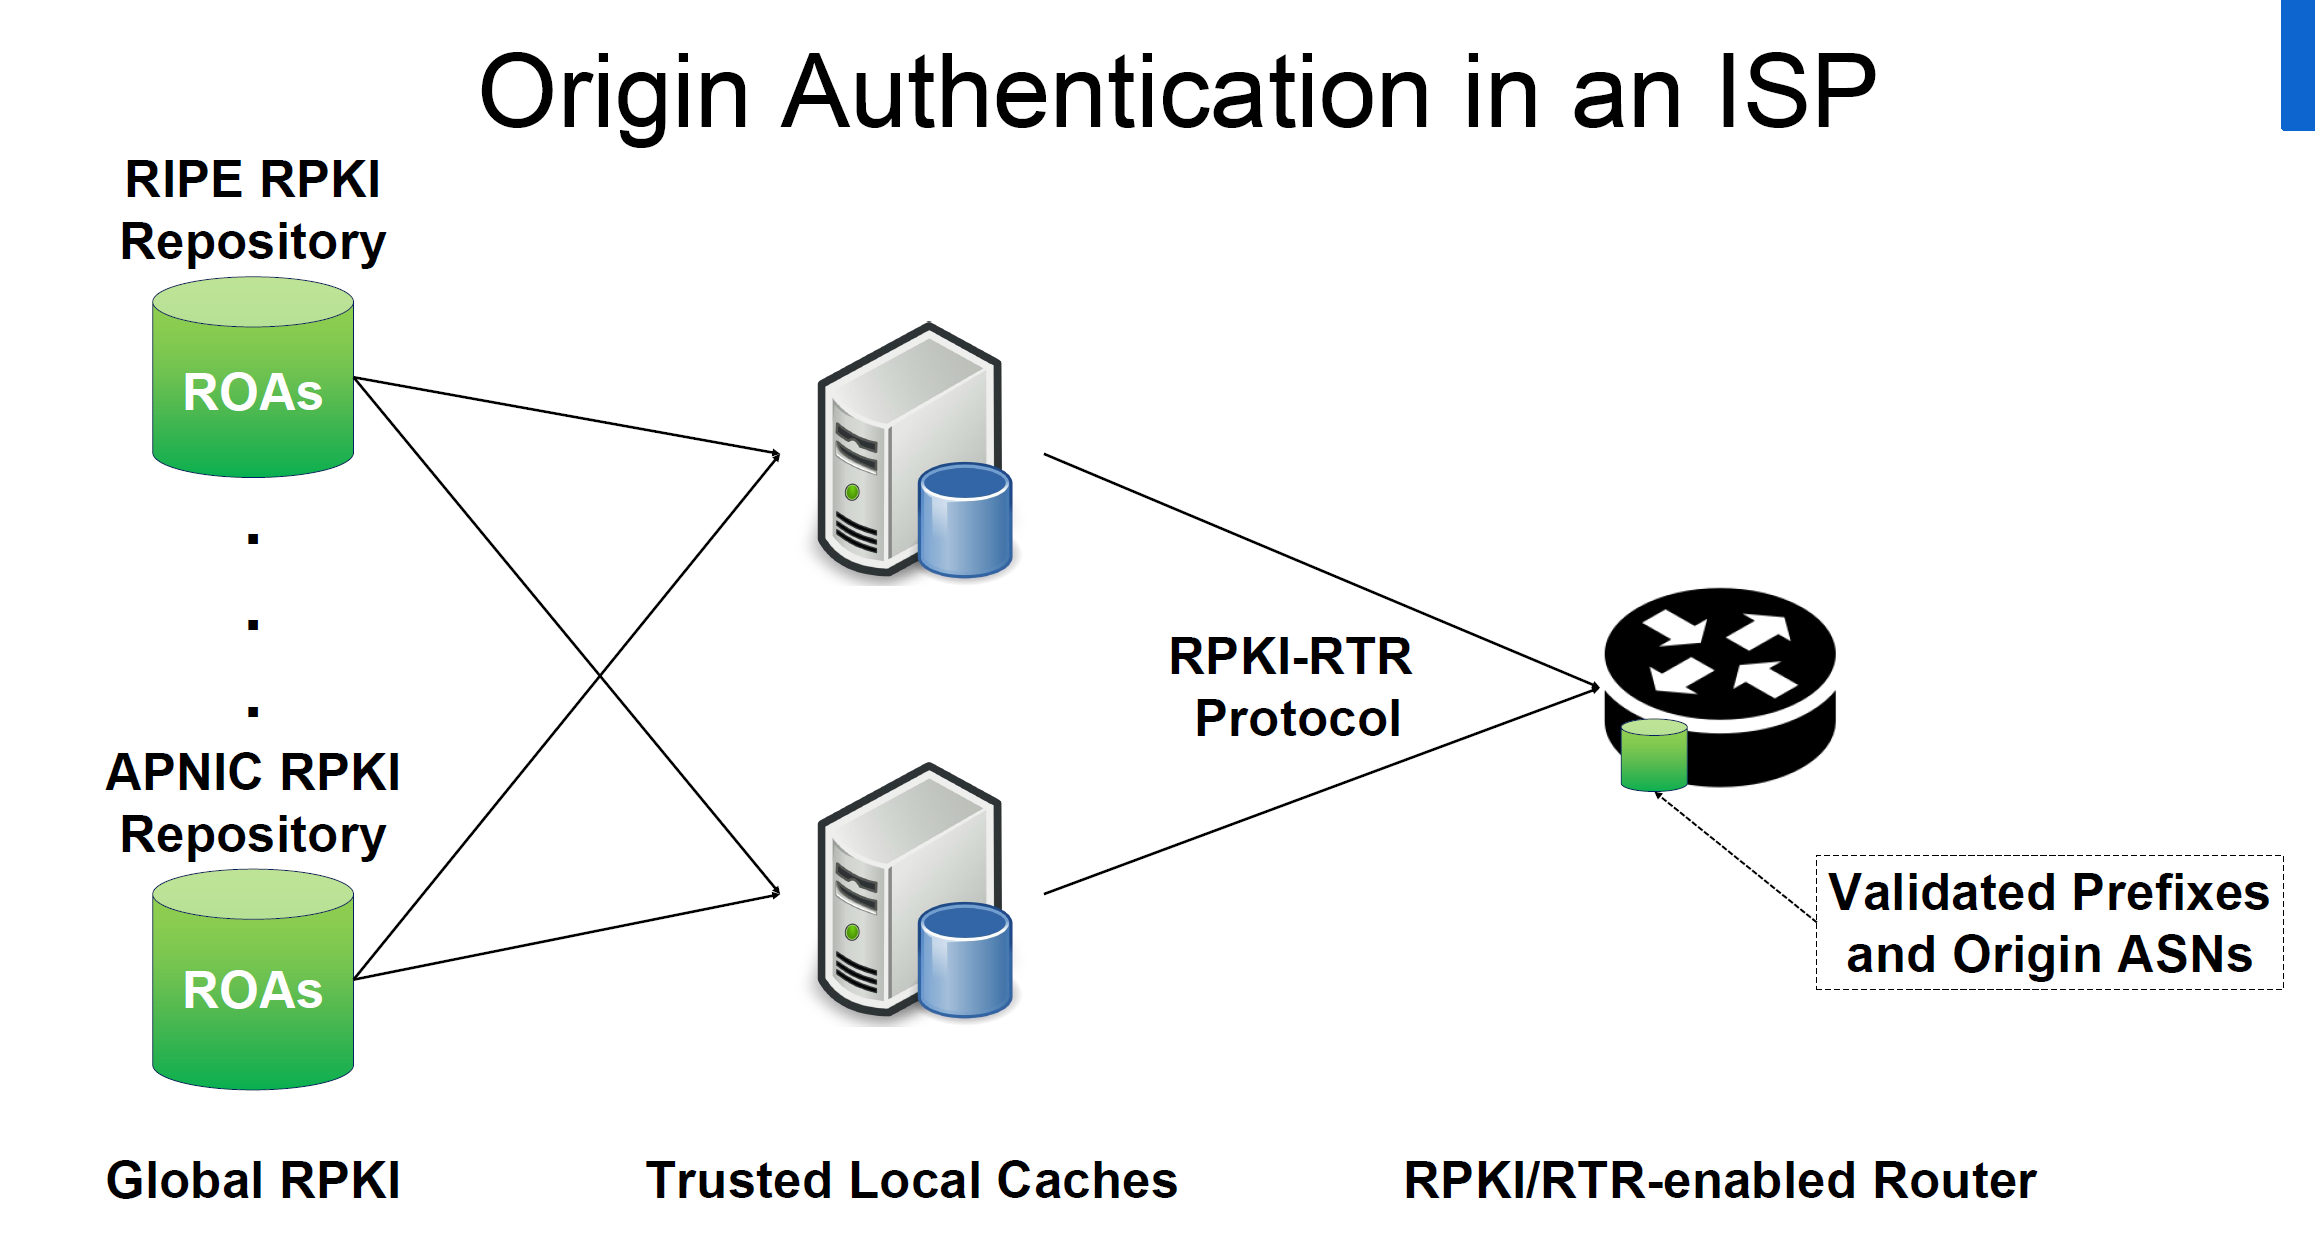
\includegraphics[width=\linewidth]{Figures/BGP_oa.PNG} 
\end{minipage}

\subsubsection{Solution to Problem 2: BGPsec}

In order to prevent the problem of ASes illegitimately appending themselves to AS paths, we need to secure the AS-path attribute, which prevents crafting a valid origin on path and path poisoning. BGPsec is trying to achieve this through Origin authentication and cryptographic signatures.\\
BGPsec signs received update message to prove that path was correctly updated and includes the next AS in the signature. This way, BGPsec can validate that the AS path indicates the order ASes were traversed and that no intermediate ASes were added or removed. RPKI is used to verify AS key material (as in origin authentication).\\

\begin{minipage}{\linewidth}
    \centering      
    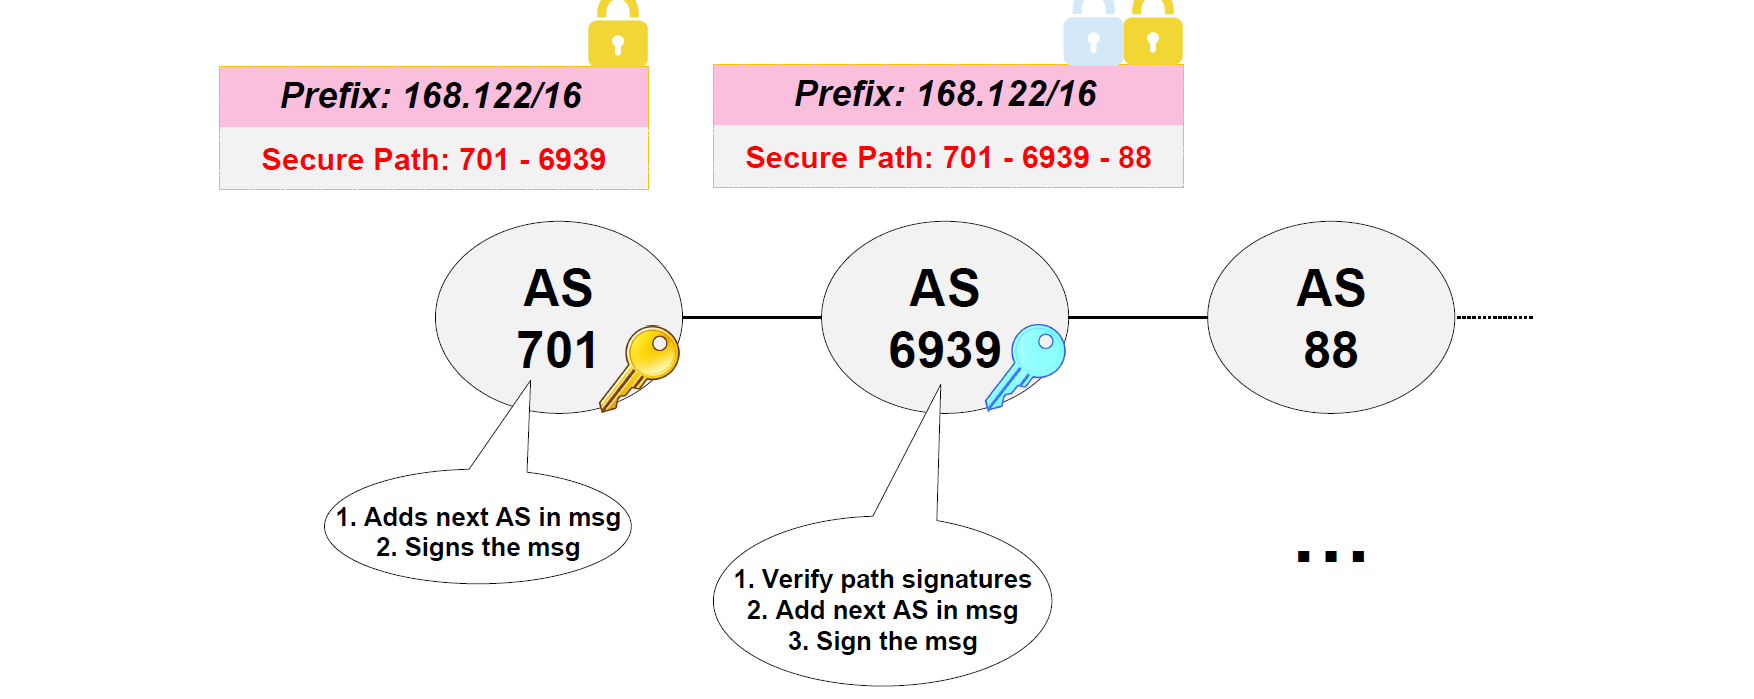
\includegraphics[width=\linewidth]{Figures/BGP_bgpsec.PNG} 
\end{minipage}

Example: AS 701 send out advertisement and signs msg with its privatekey. AS 6939 can verify the signature (pubKey of AS 701) and add the next AS to the path and again sign the message. ASes always need include the next AS on the path and then sign - otherwise there would be no link between ASes and only individual ASes are secured but not the linking between them.

\paragraph{Problems with BGPsec:}
\begin{itemize}
	\item Insecure ASes use legacy BGP, and secure ASes must accept legacy insecure routes $\rightarrow$ \textit{protocol downgrade attacks}: If operators don’t prioritize security, an attacker can just use legacy BGP to announce bogus routes to BGPsec neighbors.
	\item Routing policies can interact in ways that can cause BGP wedgies.
	\item \textit{Performance degradation}: Prefix aggregation no longer possible, since you can't sign a prefix owned by someone else. Real-time signature and validation. Slower convergence.
	\subitem $\rightarrow$ \textit{BGPsec does not scale}
\end{itemize}

\paragraph{Other Approaches: Extensive Monitoring}
\begin{itemize}
    \item Monitoring BGP update messages and use past history.
    \item Out-of-band detection mechanism
\end{itemize}

\subsubsection{Path-End Validation: Deployable Routing Security}

Important observation: AS paths today are very short! Average AS-level path length is only 3-4 hops. The basic idea is to have something between origin authentication and BGPsec. Path-End Validation tries to reduce overhead of BGPsec.\\

\begin{itemize}
	\item Origin Authentication with RPKI secures only the announced prefix. This way, no AS can announce a prefix it does not own.
	\item Path-end Validation secures the first hop	from originator to its provider. This way, no AS can simply append itself after the first AS on the AS path. Why does this work: you can still append yourself after two ASes. \textit{But} this makes the AS path rather long and thus less attractive.
\end{itemize}

This has several advantages over full BGPsec: Lower overhead, requires no cooperation from other ASes, no full deployment necessary, stronger incentive for early adopters.

\section{DDoS Attacks and Defenses}
\label{ddos}

Denial of Service (DoS) attack: attempt to consume resources which are then not available to legitimate users. Possible target resources: network links, servers, processing, storage, etc. Distributed Denial of Service (DDoS) attack is a coordinated DoS with many attackers. DDoS attacks pose a significant threat and are often used to extort companies!

\subsection{Attack types}

\begin{minipage}{\linewidth}
    \centering      
    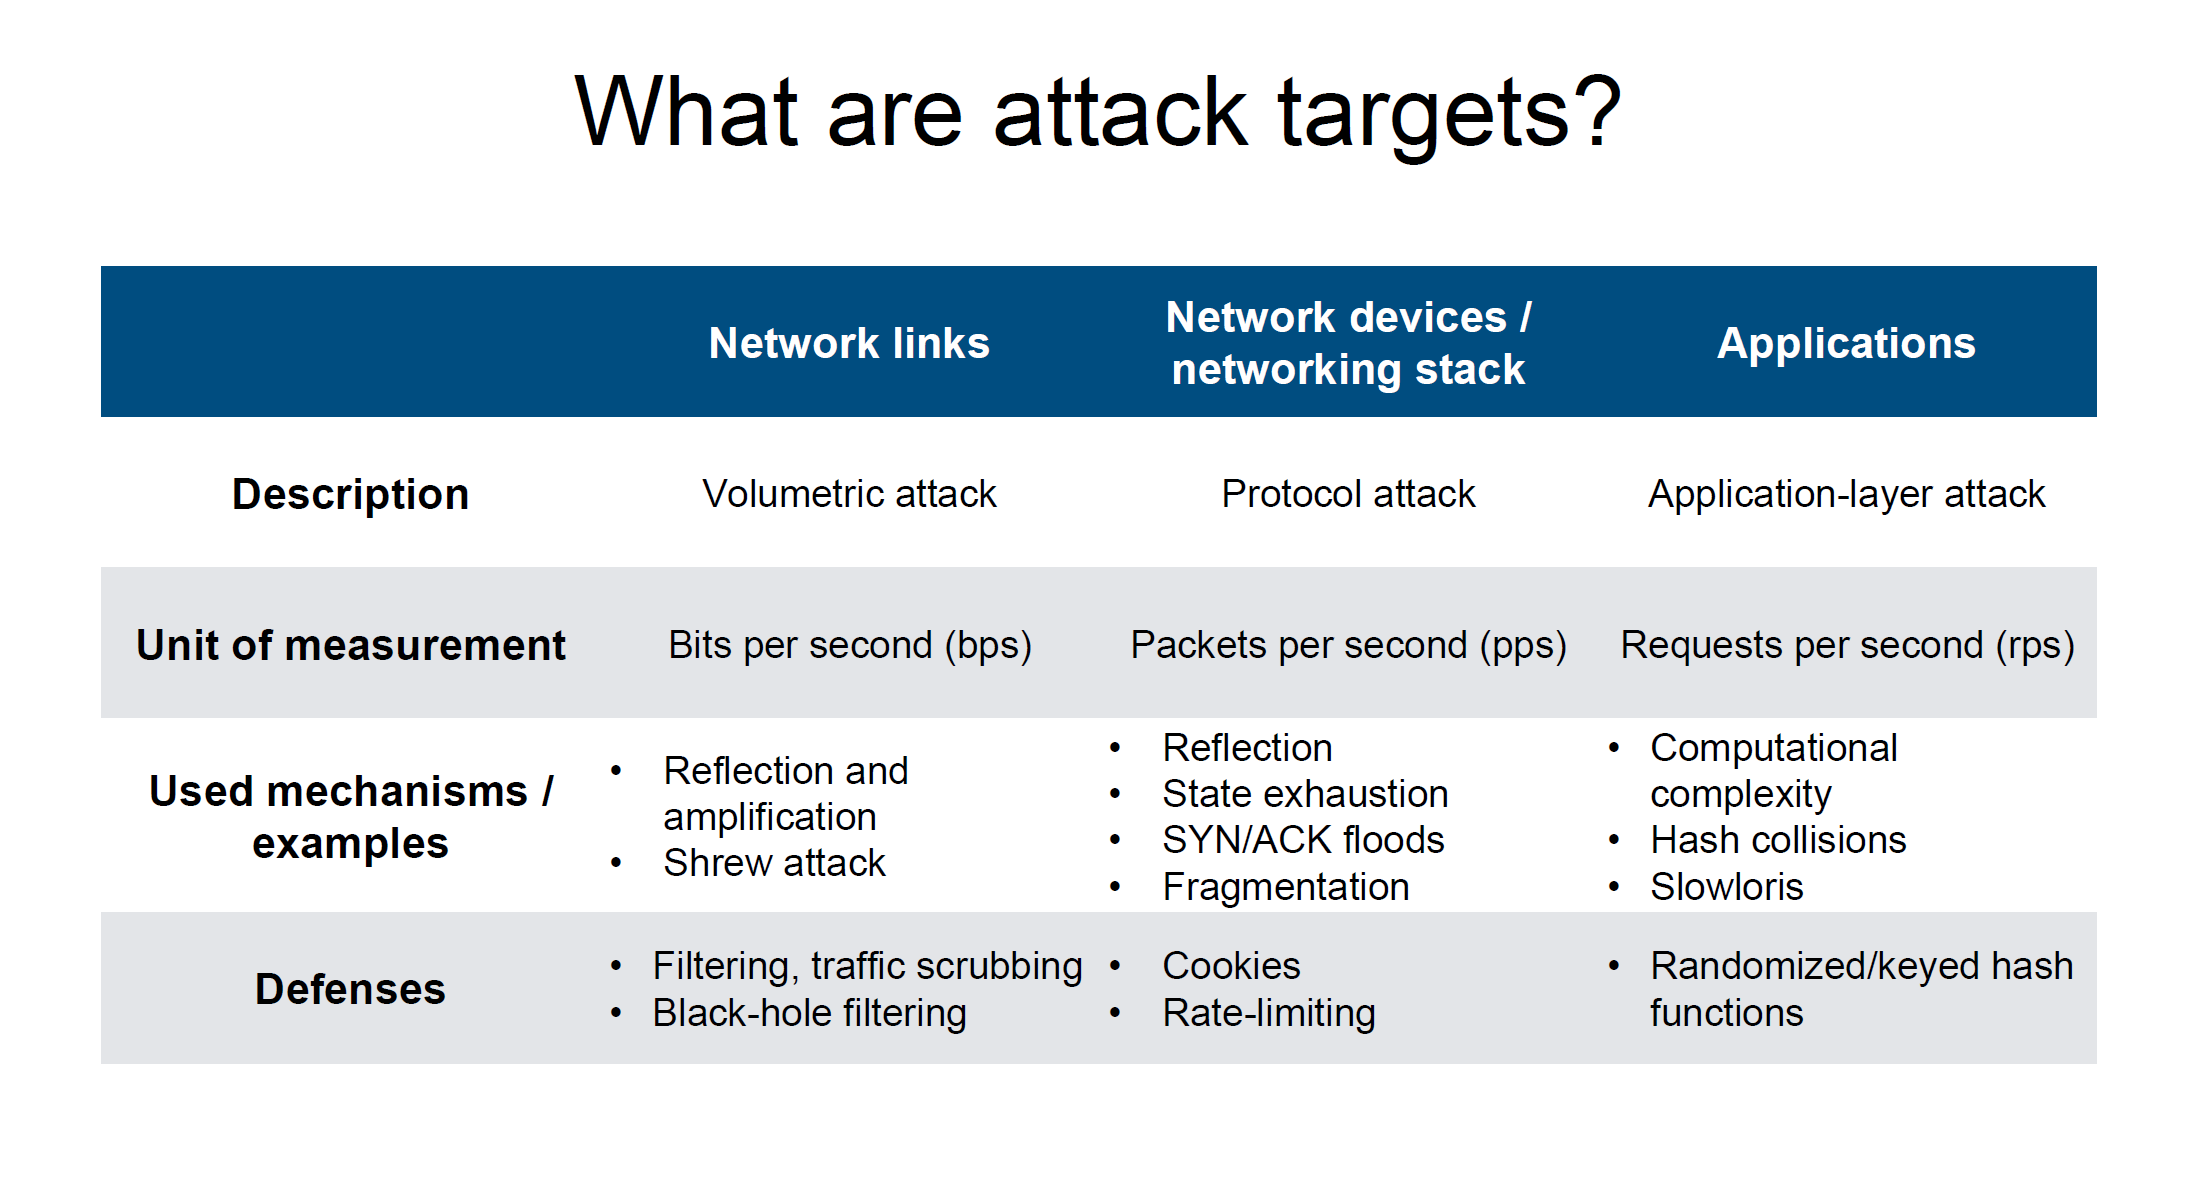
\includegraphics[width=\linewidth]{Figures/DDOS_attack_types.PNG} 
\end{minipage}

\subsection{(IoT) Botnets}
\paragraph{Botnet} 
\begin{itemize}
    \item A set of compromised machines connected to the Internet.
    \item Execute malicious code and can be controlled via command and control (C&C) systems.
    \item Often geographically distributed
\end{itemize}

\paragraph{IoT devices are perfect for constructing botnets}
\begin{itemize}
    \item Many devices with uniform configuration
    \item Often very poorly secured, hardcoded credentials.
    \item Often no security updates after few years.
    \item Often connected to internet without bandwidth limitations
\end{itemize}

\paragraph{Possible Mitigations:}
\begin{itemize}
    \item Patch: automatic security updates, provide patches for full life-time of devices.
    \item Credentials: No hardcoded credentials, force users to change default passwords.
    \item Monitoring: ISPs should actively monitor their network for suspicious traffic.
\end{itemize}

\subsection{Reflection and Amplification}

\paragraph{Address Spoofing:} Source address in IP header can be set by sender. In a connectionless protocol (UDP), server cannot confirm actual sender.

\paragraph{Defenses against address spoofing:}
\begin{itemize}
    \item Address filtering by ISPs: ensure hosts use their own addresses. Needs to be globally deployed. Poor incentives for ISP to deploy it (only other ISPs profit)
    \item Use connection-based protocols (TCP). Additional latency, potentially additional DoS attack vector (state exhaustion).
    \item Cryptographic source authentication: Additional DoS attack vector if built on expensive asymmetric crypto. Requires symmetric key distribution or PKIs
\end{itemize}

\paragraph{Reflection and Amplification:}
\begin{itemize}
    \item Requirements:
    \begin{itemize}
        \item Ability to spoof source address
        \item Publicly accessible servers
        \item Ideally response is (much) larger than request -> amplification
    \end{itemize}
    \item Typical reflectors:
    \begin{itemize}
        \item DNS (up to ~180)
        \item NTP (up to ~500) vulnerability was closed.
        \item Memcached (up to ~50000) UDP disabled by default in  version 1.5.6
    \end{itemize}
\end{itemize}

\begin{minipage}{\linewidth}
    \centering      
    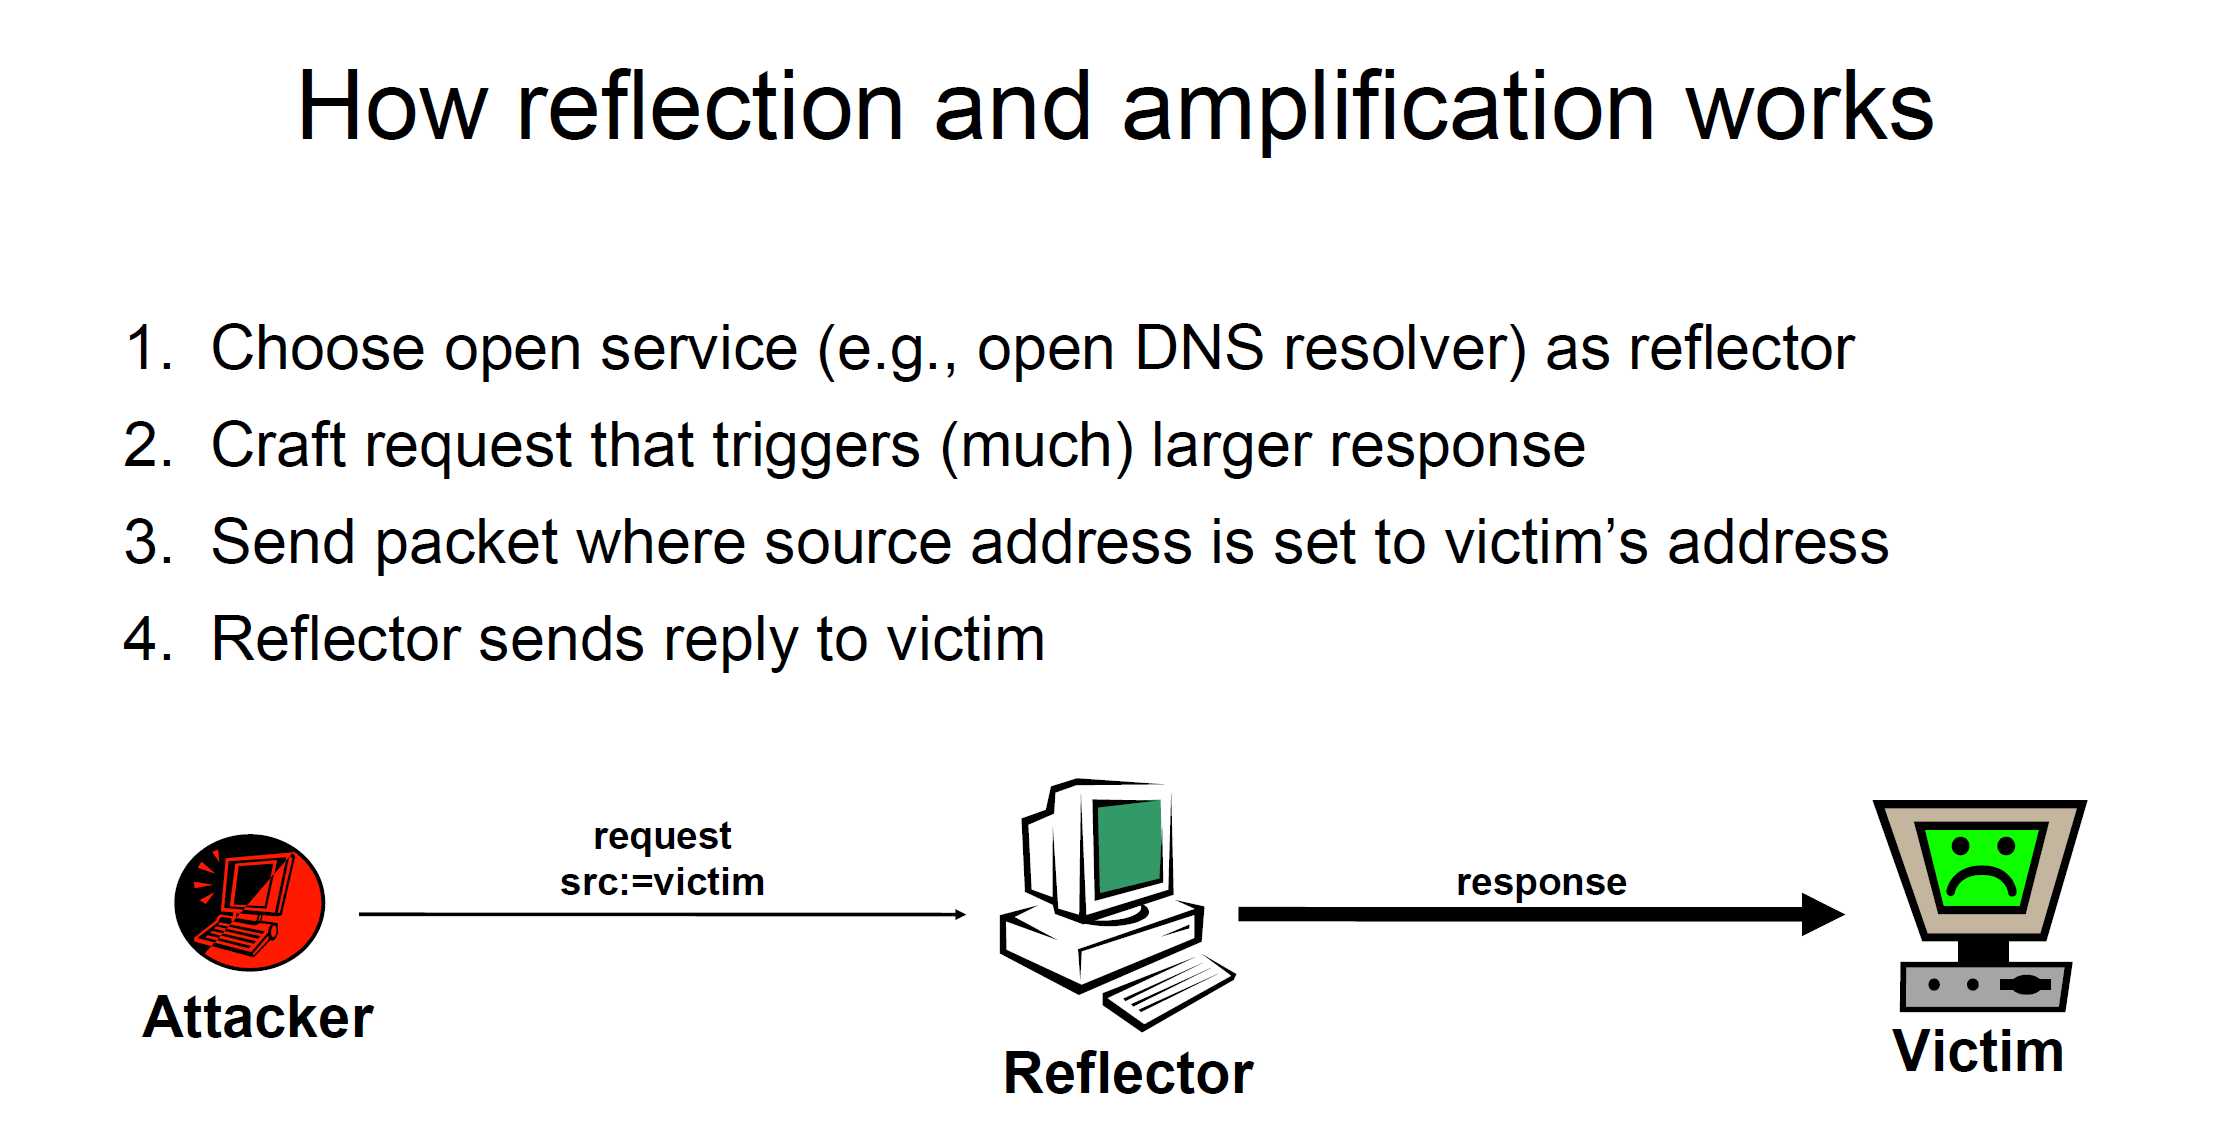
\includegraphics[width=\linewidth]{Figures/DDOS_reflection.PNG} 
\end{minipage}

\begin{minipage}{\linewidth}
    \centering      
    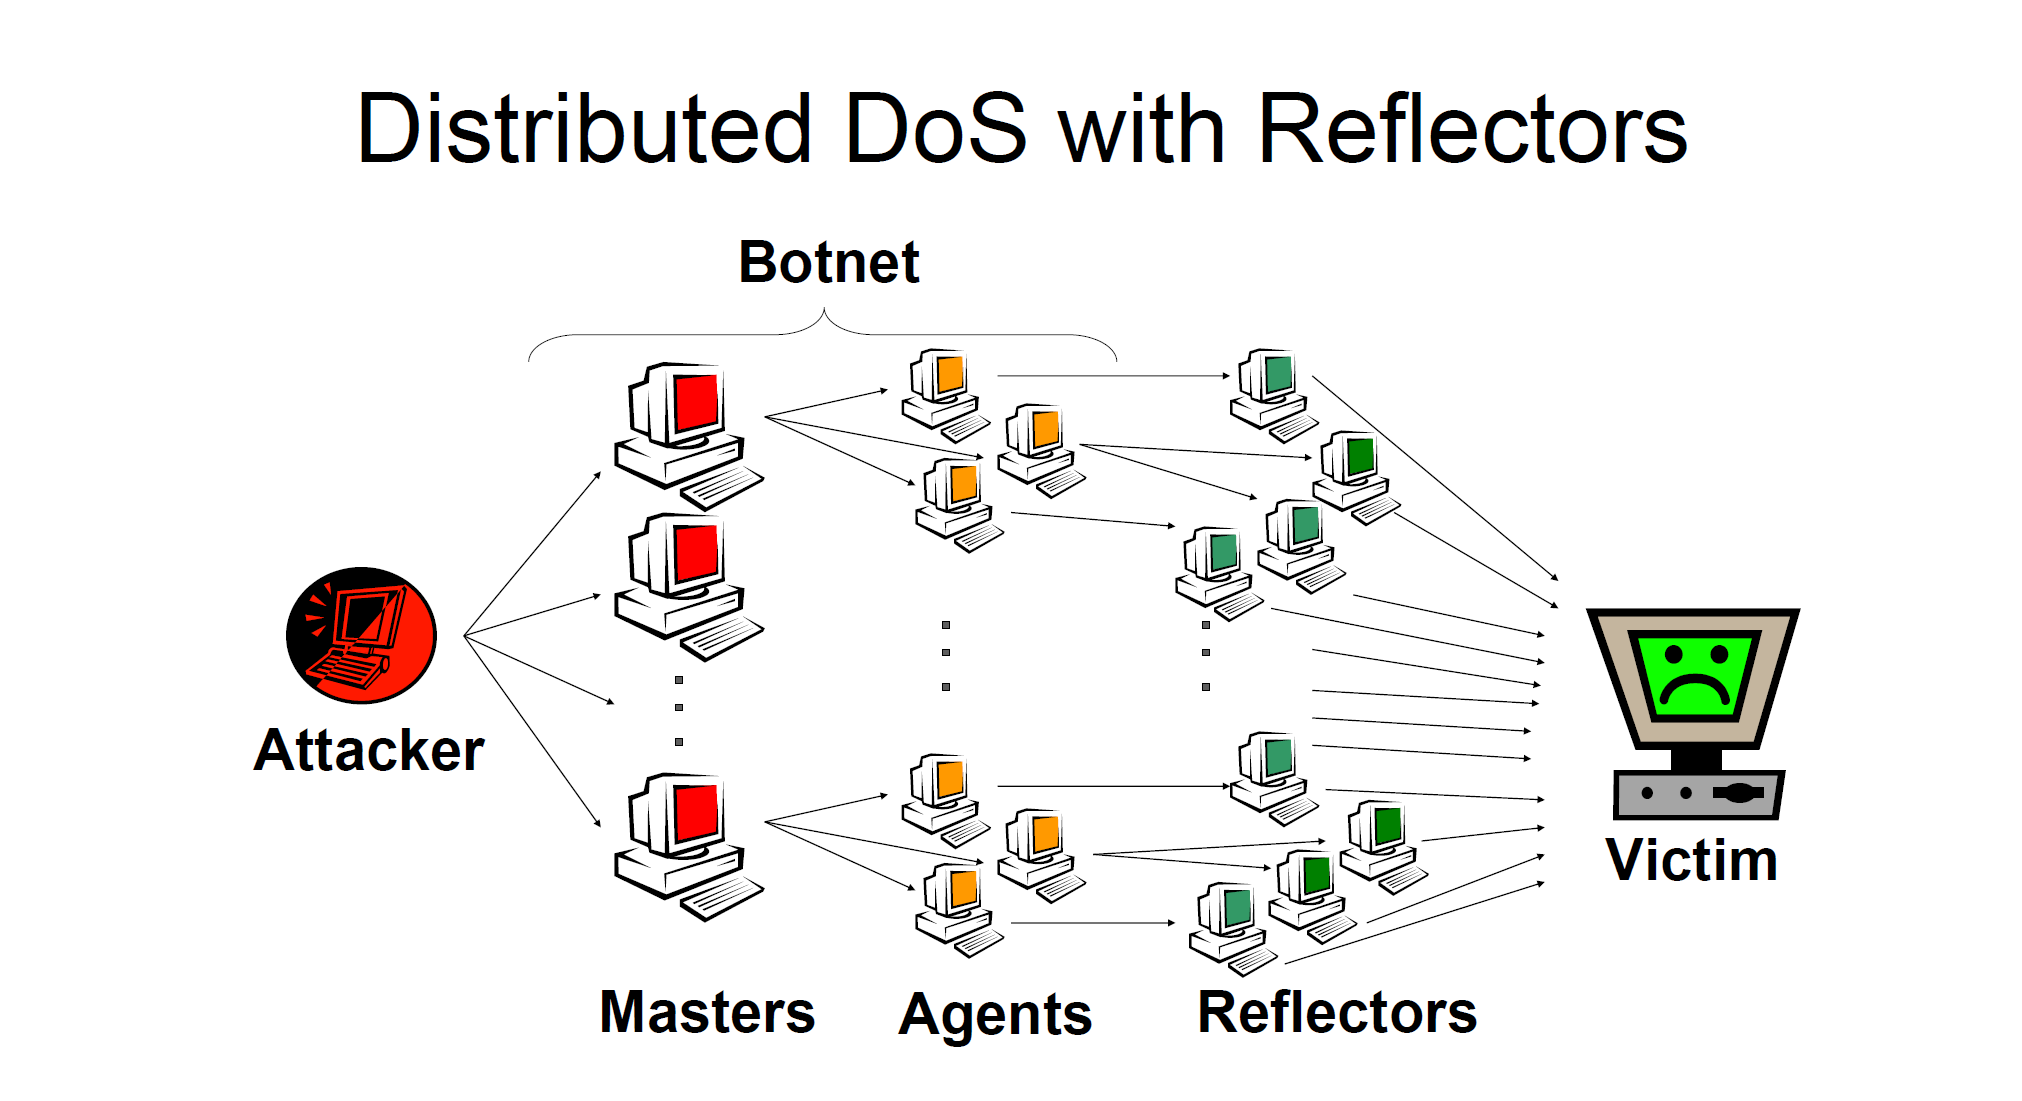
\includegraphics[width=\linewidth]{Figures/DDOS_distributed_reflection.PNG} 
\end{minipage}

\paragraph{Reflection Mitigations:}
\begin{itemize}
    \item Prevent address spoofing
    \item Perform access control (DNS servers deployed within an organization or ISP should only serve clients from this organization.
    \item Implement response rate limiting RRL (limit the nr of responses to a client)
    \item Ensure small amplifications factors (ideally < 1)
\end{itemize}


\subsection{Specific Attack Examples}

\subsubsection{Volumetric Attack: Shrew Attack}

Conventional bandwidth-based DoS requires sending high-rate attack traffic (like an elephant). Can we achieve the same effect by sending low-rate attack traffic (like a fierce shrew)? YES!\\

\paragraph{Shrew DoS Attack:} Exploits TCP congestion control feature. Researchers discovered that if you send traffic during very short but specific amounts of time, you can completely disrupt TCP. This is due to TCP congestion control resending packets at multiple whole seconds granularity (1s, 2s, 4s, 8s, ...). By only creating congestion during these time periods the attacker forces TCP flows to repeatedly enter a retransmission timeout state by sending high-rate but short-duration bursts! We deny the bandwidth of legitimate TCP flows as it makes TCP believe there is a long-term congestion.

\paragraph{Retransmission Timeout in TCP Congestion Control}
\begin{itemize}
    \item Exponential bakcoff timeout: If packet dropped retransmit in 1s, then 2s, then 4s...
\end{itemize}

\paragraph{Temporal lensing:} "multiple rounds simultaneous impact”. Use time as an additional amplification factor. Different paths have different transmission delays. An attacker can send packets at different times s.t. they \textit{all} arrive at the target \textit{at the same time}. So that a low-bandwidth source can also perform a shrew attack.

\subsubsection{Volumetric Attack: Coremelt and Crossfire}

Both of these attacks haven't been seen in the wild yet but are theoretically possible.

\paragraph{Coremelt attack}

\begin{itemize}
    \item Adversary controls many bots distributed across the Internet.
    \item Bots send traffic \textit{between each other}, thus all traffic they produce is legit traffic desired by the destination (destinations are bots). Traffic is not sent to a victim as in regular DDoS attacks. Thus, all defense methods discussed before do not work here.
    \item Adversary can exhaust bandwidth on victim link.
    \item As a result, the attack traffic exhausts bandwidth in per-flow fair sharing systems.
\end{itemize}

\paragraph{Crossfire attack}

\begin{itemize}
    \item Adversary controls distributed bot army
    \item Observation: due to rout optimization, few links are actually used to connect a target region to rest of internet. 
    \item Adversary can contact selected servers near/in target region to overload target links.
    \item Result: disconnect target region from remainder of Internet.
    \item Hard to stop since only connection establish packet (TCP SYN) are sent.
\end{itemize}

\subsubsection{Protocol Attack: DNS FLooding}

\paragraph{NXDOMAIN Attack}
\begin{itemize}
    \item Goal: overwhelm victim's authoritative name servers.
    \item Idea: query many non-existent subdomains of victim domain.
    \item Resolver queries all authoritative name serverss in turn
    \item Can use multiple DNS resolvers
    \item Can be sent from distributed botnet and via many different DNS resolvers.
    \item Result: name server can no longer reply to legitimate requests.
\end{itemize}

\paragraph{Why is this a problem?}
\begin{itemize}
    \item Most internet-based services rely on DNS to map domain names to IP addresses.
    \item If a domain name cannot be resolved, the service does not work.
    \item A DoS attack on the DNS system makes many additional systems unavailable.
\end{itemize}

\subsubsection{Protocol Attack: Session State Exhaustion}

\paragraph{Session State Exhaustion}
In a two way communication, each channel between peers needs a unique session number. This session number has to be known at the server to match requests to the right session/ channel. Keep in mind that servers have limited memory.\\
\noindent\textbf{Attack:} Exhaust the session table of the server.\\
\textbf{Result:} Server can no longer accept new connections, existing connections are dropped, maybe the server/service crashes.

\paragraph{SYN Flood Attack}
TCP uses a three-way handshake to establish a connection. The client initiates the handshake by sending a SYN packet. The server stores a new state for the received SYN packet.\\
\textbf{Attack:} The attacker can send lots of TCP SYN packets with spoofed srcIP. The server tries to keep state for every single packet. Eventually, the state table overflows and the server is unable to accept new legit connections. For each second where the packet is in buffer, its TTL is decreased by 1. It thus takes 255 seconds until the state is dropped.\\
\textbf{Mitigation:} SYN Cookies - no state table needed. Server doesn't create session state for TCP SYN packet. Instead, the server replies with SYN+ACK and a cookie (sequence number) $B=F(time,IP,port,...)$. On the next reply, the server then checks if the client sent $B+1$ along. Attacker can just send the cookie too...? No! Since the srcIP is typically spoofed, the attacker won't receive the cookie. The attacker could try to spoof the cookie (if she knows the function F...). The server should use cryptographic hashes or salted hashing such that the attacker can only guess $B$.

\paragraph{Generic Mitigations}
\begin{itemize}
    \item Attack: The attacker aims to exhaust session state of a protocol/application at server.
    \item Countermeasures:
    \begin{itemize}
        \item Encode state in a unique but determined way that allows the server to validate the state in the reply.
        \item No need to store session state at the server.
        \item Ensure the encoding cannot be tampered (use crypto-hashes, unique data known to server only)
        \item Server generates B = Hash(salt, A) where salt is known to server only and changes over time
        \item Server only needs to store a few salt values to validate replies.
    \end{itemize}
\end{itemize}

\subsubsection{IP spoofing defense}

\begin{itemize}
	\item Ingress Filtering: at network edge, outgoing packets with incorrect srcIPs are filtered (e.g. ETH filters packets whose srcIP is not within the ETH prefix). All ISPs should do this (in reality only 30\% do).
	\item iTrace: One in 20,000 packets “triggers” a router to send a special packet with route information sent to both src and dst. DDoS victim could reconstruct attack paths. But extra packets waste bandwidth.
	\item Packet Marking: Routers mark 16-bit IP ID field with information that enables reconstruction of IP address. This has no overhead but probabilistic marking often requires ca. 1000 packets.
\end{itemize}

\subsubsection{Application-Layer Attack: Algorithmic Complexity Attack}
Algorithms often have good average case running times but bad worst case running times (for certain inputs) (e.g. quicksort or hashtable lookup).\\
An attacker can exploit this by sending special inputs that trigger worst-case running times of algorithms.

\paragraph{Hash table lookup: Countermeasures}
\begin{itemize}
    \item Universal Hashing: Hash functions guarantee 0 or low collision for any input
    \item Hash randomization: Harder for attacker to find out the worst-case input. E.g. use a secret hash function for each hash table.
\end{itemize}

\subsubsection{Regular Expression Denial of Service (ReDoS)}
There are "malicious" inputs to certain regular expressions that take a very long time to evaluate. A server could become unresponsive when facing such a regex.\\
Example: input aaaaaa!@gmail.com to:\\
\texttt{([a-zA-Z0-9])(([\-.]+)?([a-zA-Z0-9]+))*(@){1}[a-z0-9]+[.]{1}(([a-z]{2,3})| ([a-z]{2,3}[.]{1}[a-z]{2,3}))}

\subsubsection{Application-Layer Attack: Slowloris}
Slowloris allows a single machine to take down another machine's web server with minimal bandwidth and side effects on unrelated services and ports.\\
\textbf{Basic idea:} Slowloris tries to keep many connections to the target web server open and hold them open as long as possible. Periodically, it will send subsequent HTTP headers, adding to - but never completing - the request. This will fill the maximum concurrent session pool of the server, eventually denying additional connection attempts from clients.\\

\paragraph{Mitigation:}
\begin{itemize}
	\item increase the maximum number of clients the webserver will allow
	\item limit the number of connection per srcIP
	\item put a lower bound on the transfer speed (might lose some customers with very slow internet), but this forces the attacker to spend at least some resources
	\item put an upper bound on the connection time (again, might lose some legitimate customers)
	\item setup reverse proxies, firewalls, load balancers or content switches
\end{itemize}

\subsection{DDoS Defense Mechansims}
\begin{itemize}
    \item Ingress filtering: Removes packet with illegiimate source IPs
    \item Computational puzzles: Slows down attacks, achieves per-computation fairness
    \item Cloud- or ISP-based filtering
    \item Network capabilities: Allows victim to block unwanted traffic closer to the src
    \item IP traceback: Reveals the real source IPs of packets.
    \item No single point of failure, more than two geographically diverse locations, more than two independent Internet connections
    \item Long term monitoring: to assess periodicity and peak periods/loads.
    \item Over Provisioning: Plan bandwidth and resources to cover the majority of extreme peak loads
\end{itemize}

\subsection{In-network and Cloud-based DDoS	Mitigation Services}

\subsubsection{Cloud-based DDoS Mitigation Service}
Cloud/CDN providers such as Akamai or Cloudflare offer DDoS mitigation. By changing BGP or DNS of web server, the traffic is redirected to the provider as a middle-man (e.g. use BGP anycast to have the same IP address at different places). Some provide Content Delivery Network (CDN) service to achieve diversion of traffic. This is today's state of the art.

\subsubsection{ISP-based DDoS Mitigation Service}
Upon detecting a DDoS attack, ISP redirects \textit{entire} traffic destined to victim to the scrubbing center, then send good traffic back to the destination. Scrubbing center keeps state for each connection (lots of machines) and uses Deep packet inspection (DPI) and connection pattern to filter malicious traffic. Parts of the detection algorithm is signature based (needs frequent updates).

\subsubsection{Discussion: Cloud- or ISP-based Filtering}
\begin{itemize}
	\item Cloud-based security provider can be easily bypassed: Because most cloud use DNS to redirect traffic, attackers can easily bypass the proxies if the victim’s IP is exposed.
	\item Privacy violation: E.g., Radware decrypts HTTPS and injects CAPTCHAs to client. An untrusted or compromised cloud could expose users’ sensitive data.
	\item Very limited destination traffic control
	\item High cost for small-, medium-size organizations
	\item Requires continuous subscription for fetching attack signatures
\end{itemize}

\subsection{Remotely Triggered Black Hole Filtering (RTBH)}
RTBH is a generic technique that can be used to mitigate volumetric DoS attacks - the offending traffic is simply dropped (black-holed) at the border routers of an AS. RTBH comes in two flavors, source-based and target-based.

\begin{itemize}
	\item source-based RTBH: All traffic from attacker's subnet is dropped by target's ISP
	\item destination-based RTBH: All traffic to the target’s subnets is dropped by the target’s ISP\\
\end{itemize}

RTBH will drop traffic at the border routers, so that the traffic does not even enter the AS. The main solution is to sink all traffic that is destined to a particular placeholder IP address, chosen among an unused subnet. The subnet usually chosen is 192.0.2.0/24, technically reserved for testing purposes. Let’s say that we want all traffic destined to 192.0.2.1 to be dropped: we will then create the following static route. \texttt{ip route 192.0.2.1 255.255.255.255 null0}.\\
The RTBH will be triggered by an admin that will insert route updates that route traffic destined to the
attacked IP to the placeholder IP, 192.0.2.1 . These routes will then be propagated via iBGP to the edge routers, effectively making them send all the attack traffic to \texttt{null0}.






\section{Firewalls, Intrusion Detection \& Evasion}

\subsection{Firewalls}

A firewall is a system used to protect or separate a trusted network from an untrusted network, while allowing authorized communications to pass from one side to the other.

\begin{itemize}
	\item \textbf{Network Firewall:} Network firewalls are a software appliance running on specific hardware or as virtual instance that filter traffic between two or more networks. Protect different network segments.
	\item \textbf{Host Firewall:} Host-based firewalls provide a layer of software on one host that controls network traffic in and out of	that single machine. Protect single machine
\end{itemize}

\paragraph{Hostbased vs Network:} Host based firewalls have context, know exactly what is running on a host. This allows for more fine-grained decisions. Host based firewalls are good for mobile devices (e.g. phones). Network firewalls are good if you e.g. can't install a firewall on a device (e.g. printer).

\paragraph{Filtering Rule:} Firewall rules are processed in order: the first rule that matches is picked. Thus, ordering of rules is very important.
\begin{itemize}
    \item Ingress: Filter incoming traffic (from low security to high security)
    \item Egress: Filter outgoing traffic (often gets forgotten)
    \item Default Policy: Define what to do when no rule matches (default accept vs. default reject)
    \item Deny Access: Tehniques to deny access: DROP silently drop packet (port scanner think its open), REJECT drop packet and inform sender (ICMP message).
\end{itemize}

\paragraph{Firewall State:}
\begin{itemize}
	\item \textbf{Stateless Firewall:} look at each packet on the network layer individually, no state maintained. Decisions based on packet header information. This is fast, scalable and simple but very limited.
	\item \textbf{Stateful Firewall:} keep also track of the state of the network connections, decision also based on session state. This is more powerful but: state explosion, inconsistencies, state for UDP? The problem with state explosion: an attacker can exhaust the memory of a firewall. Then, the default rule matches: if default accept: all traffic is allowed. If default deny: server is DoSed.
\end{itemize}

\paragraph{Evolution of Firewalls:} The legacy firewall technology is effectively blinded by the evolution:
\begin{itemize}
    \item Firewalls can't block all malicious traffic, many ports must be kept open for legitimate applications.
    \item Users unwittingly download dangerous applications or other forms of malicious code
    \item Peer-to-peer and instant messaging have introduced new infection vectors.
    \item Web 2.0 trends push critical business applications through firewall ports that were previously reserved for a single function (e.g. HTTP)
\end{itemize}

\paragraph{Next Generation Firewall (NGFW)}

\textbf{Functionality:} deep packet (content) inspection, take application and protocol state into
account for security decision. This allows for even more powerful rules, protocol and application awareness but requires support for many (badly documented) protocols, has performance and scalability issues and introduces inconsistencies between host/app and FW.

\paragraph{Web Application Firewall (WAF)}

Protect web-based applications from malicious requests. Request filtering: request pattern, SQL injection, XSS, buffer overflow attempts, etc. Often implemented as a reverse proxy. Static or dynamic blacklisting/whitelisting. False positive problem. WAF's are often implemented as a reverse proxy to protect public facing web applications. Reverse Proxy: client accesses reverse proxy without knowing internal network. Reverse proxy then manages resources from internal network for client.

\paragraph{Organizational Challenges}

Managing and maintaining firewall rules in a company is challenging. Firewall rules are complex and if the employee that created them leaves, someone else has to understand the monster. Further, security and network operation teams have opposing interests: security team wants to provide secure access, network team wants to provide high availability.

\paragraph{}{Firewall Attack Methods}
\begin{itemize}
    \item IP Source Spoofing: spoofing src addr to bypass filters
    \item Artificial Fragmentation: of packets to bypass rules (firewall needs to reassemble to understand content), also out of sequence sending of fragments.
    \item Denial of Service: Firewall state explosion, whats fallback policy?
    \item Encodings: Different encodings and addition of noise (different obfuscation techniques). Undefined or border cases are very effective for detection evasion.
    \item Vulnerabilities: Firewalls are complex software, which are riddled by vulnerabilities as any other software product.
\end{itemize}

\subsection{Intrusion Detection \& Prevention}

Protecting a large number of hosts, end-points, or network segments is not trivial.
\begin{itemize}
    \item Reactive: system can only detect already known attacks
	\item Proactive: system can detect known and yet unknown attacks
	\item Deterministic: system always performs the same given the same input (blacklist, signatures)
	\item Non Deterministic: system detection is fuzzy (heuristics, machine	learning, sandboxing) and depends on current state of the world. The reason for alert is typically not known.
\end{itemize}

\paragraph{Detection Techniques}

\begin{itemize}
    \item Protocol Analysis: Analysis and decoding of protocols. Reassembly and normalization of traffic
	\item Signature based systems (static): Promptly identify and label threat. But I can only identify threats that I've already seen before. For each new threat, a unique signature or signature artifact is created by a skilled engineer or security researcher. Frequent updates to signature database or online lookups.
	\begin{itemize}
		\item One-Dimensional: blacklist/ whitelist (e.g based on MD5 hashes). This is fast and low rate of false positives. But it's reactive and needs frequent updates.
		\item Two-Dimensional: classic regular-expression functions and string matching. This is more flexible and has low FPR and low/medium resource requirements. More flexibility but it's still reactive and needs frequent updates.
		\item Multi-Dimensional: instead of triggering on a single signature, a	multi-dimensional signature was created. More efficient and effective than single approach. hybrid of two above methods
	\end{itemize}
	\item Sandboxing: Run (potential) malware in a VM and examine its behavior. This is proactive and doesn't need signature updates but is resource intensive and difficult to scale. Malware can further evade sandboxing (e.g. malware could wait for 3 days before becoming malicious).
	\item Machine Learning: Apply supervised and unsupervised machine learning algorithms to detect malicious traffic, malware, etc. Problem with SL models: training data \textit{needs} to be clean (no unknown attacks), otherwise the SL model learns something wrong. With USL models, interpretability is an issue (also with SL).
\end{itemize}

\paragraph{Decision Making}

This faces many challenges: encrypted traffic (can't inspect content, only headers and statistical analysis), high number of false positives, high link speeds, induced latency, application level attacks (JavaScript, ..), etc.
\\
Accurate = right direction, on target. Precise = clustered values with low scatter.\\

\textit{“It is better to be roughly right than precisely wrong.”}\\

\begin{itemize}
	\item \textbf{0\% FNR:} Always predict 'Attack!'
	\item \textbf{0\% FPR:} Always predict 'No attack!
\end{itemize}

The difficulty: Build a detector with optimal balance between FP and FN. FNR and FPR should never be considered in isolation. Ideally, consider a joint detection metric such as the F1 score.\\
Accurate detection is very challenging when rate of attacks is very low. If we have lots of traffic but very few attacks, we'll have lots of false positives, which lowers trust in the detector. 

\paragraph{Detection Evasion}

\paragraph{Malware Development Lifecycle}
\begin{enumerate}
	\item Develop new malware with desired functionality
	\item Automatically create numerous permutated samples of the initial malware at massive scale:
	\item Protect samples from analysis:
	\begin{itemize}
		\item Use \textit{crypter} to encrypt malware s.t. detection systems and static analysis processes are ineffectual.
		\item Upon execution only decrypt sections of code that are in the process of being executed on the victim’s computer.
		\item Use \textit{packers} to make binary files smaller (faster infection), make it more difficult for AV to detect malicious payload. Advanced packers employ polymorphic output capabilities (restructure malware binary everytime it's executed)
	\end{itemize}
	\item Make samples aware of sandboxing/detection technologies
	\begin{itemize}
		\item Use \textit{protector} to add anti-debugging features to malware that prevent security researchers and automated sandbox analysis technologies from dissecting samples.
		\item “protector” technology was originally designed as a DRM protection technology
		\item Protectors detect the use of debuggers or virtualization techniques if seen, the malware then causes different operations
	\end{itemize}
	\item Quality Assurance: Test samples against all current anti-malware solutions before deployment (if sample is detected by antivirus: \texttt{goto 2}):
	\begin{itemize}
		\item Check if the malware is detected by common AV software. Only testing services that do not submit malware samples to antivirus vendor are used (otherwise the malware would already be known).
	\end{itemize}
\end{enumerate}

The malware used in a targeted attack will not be detected by anti-malware tools at the time of attack because it was tested beforehand.

\paragraph{Polymorphism Techniques}
Mutate code while keeping the original algorithm intact. Swapping equivalent code constructs, changing the order of code, insert noise, compiler modulation. Also swapping of registers, reordering of instructions and defining functions in a different order.

\textbf{Binders:} Binders are used by malware authors to “embed” and Trojan other software packages (e.g. add trojan to Adobe Photoshop torrent). This helps to propagate malware, trick users into downloading and executing seemingly legit software. 

\paragraph{Attack Detection \& Defense Effectiveness}

\begin{itemize}
    \item Unable to inspect encrypted traffic
    \item High number of false positives
    \item Latency introduced by inspection engine
    \item Application level attacks (JavaScript,...)
    \item Policy/signature management
\end{itemize}

\begin{minipage}{\linewidth}
    \centering      
    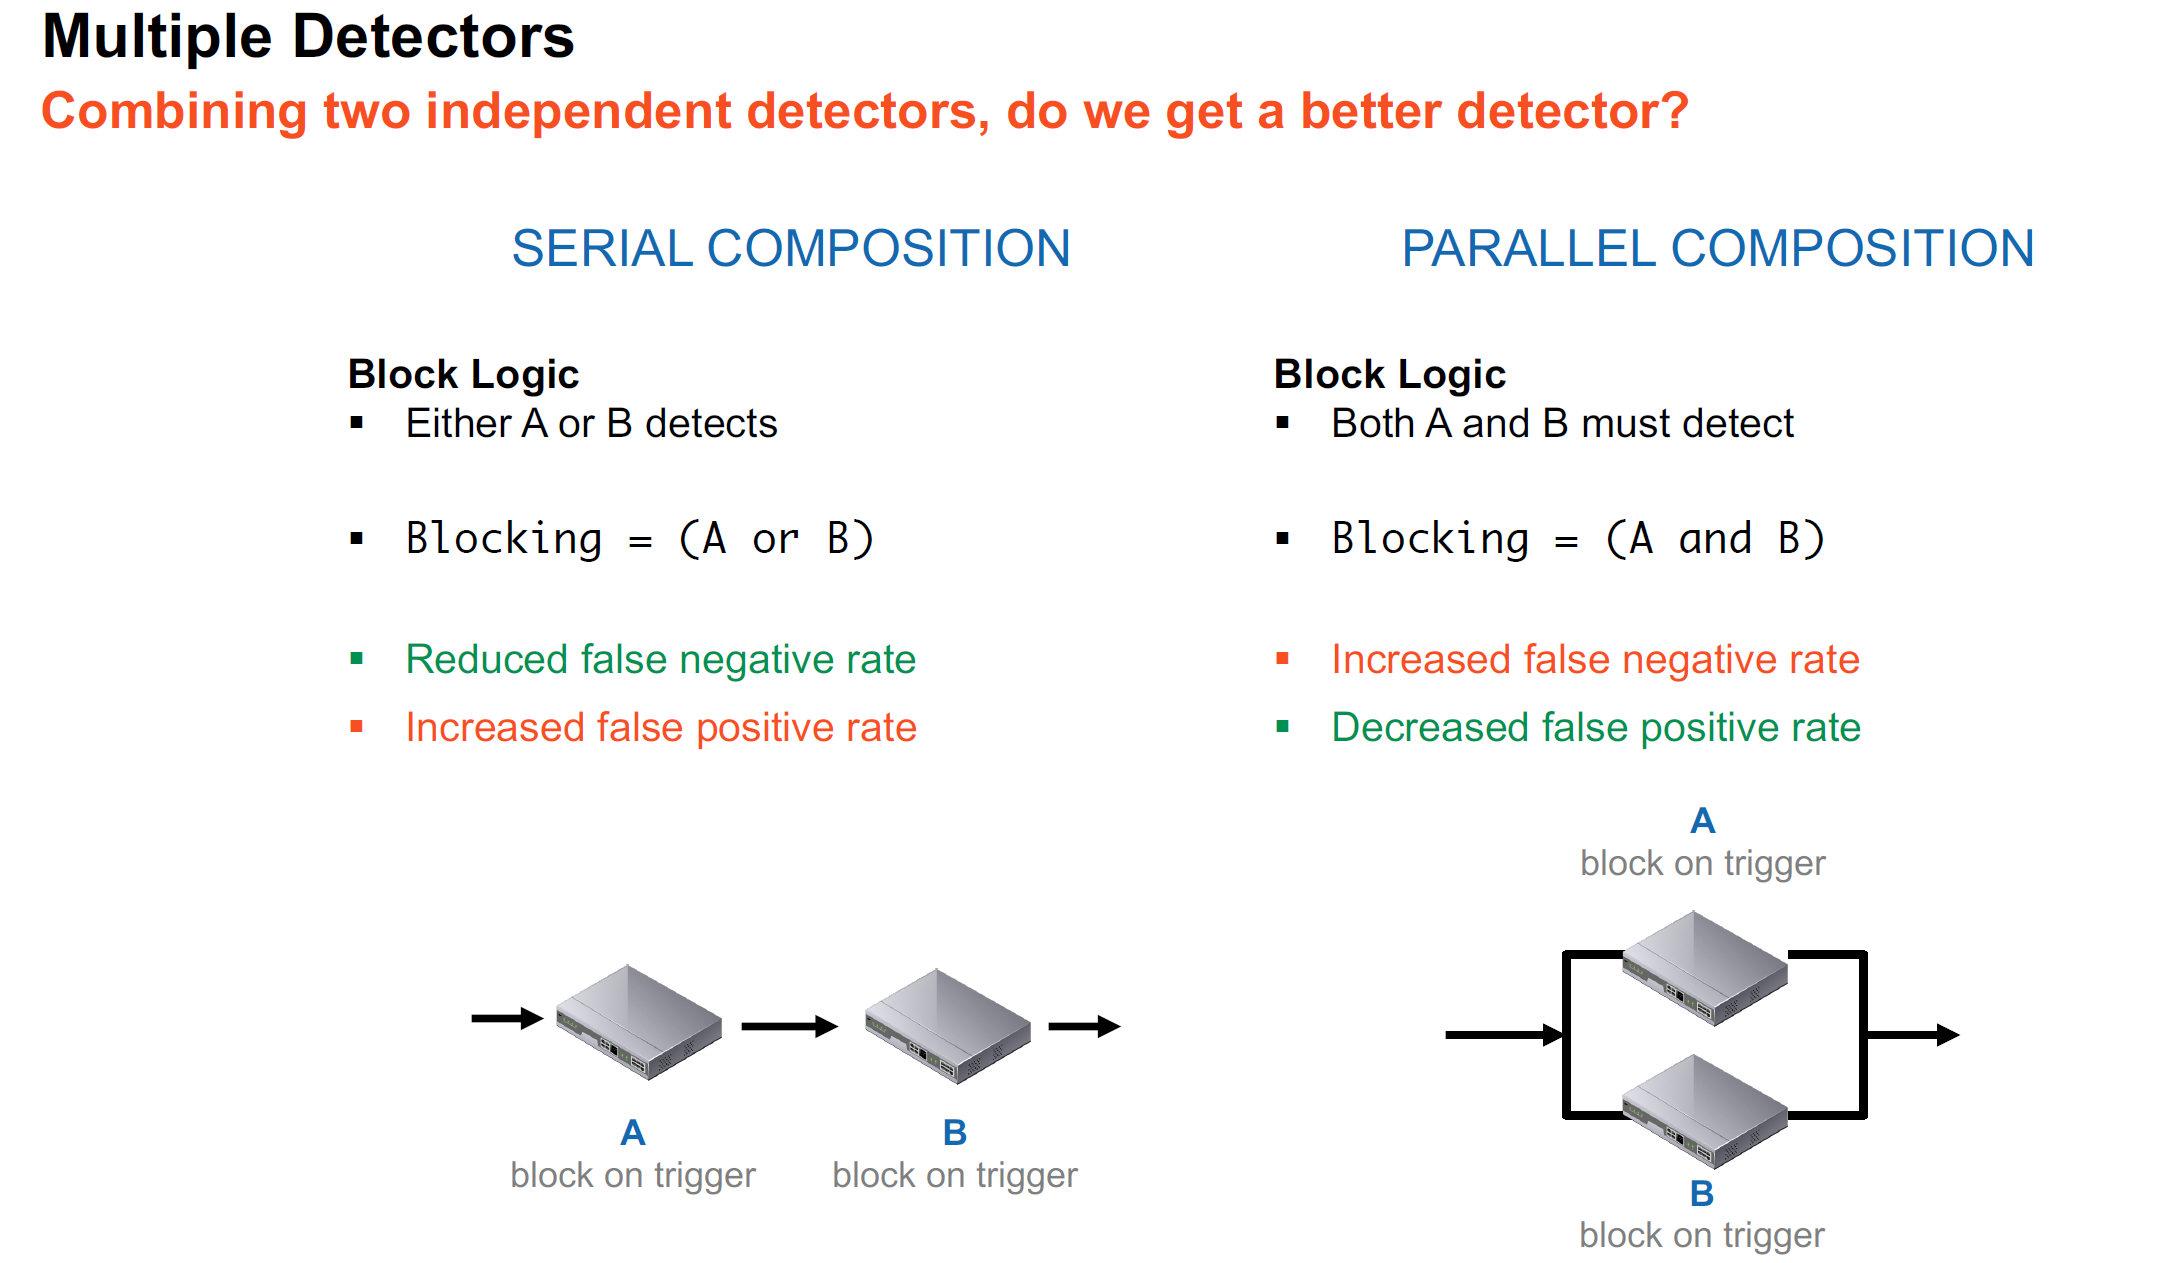
\includegraphics[width=\linewidth]{Figures/IDS_mult_detectors.PNG} 
\end{minipage}

\subsection{Layered Security Filtering and Protection:}

\begin{minipage}{\linewidth}
    \centering      
    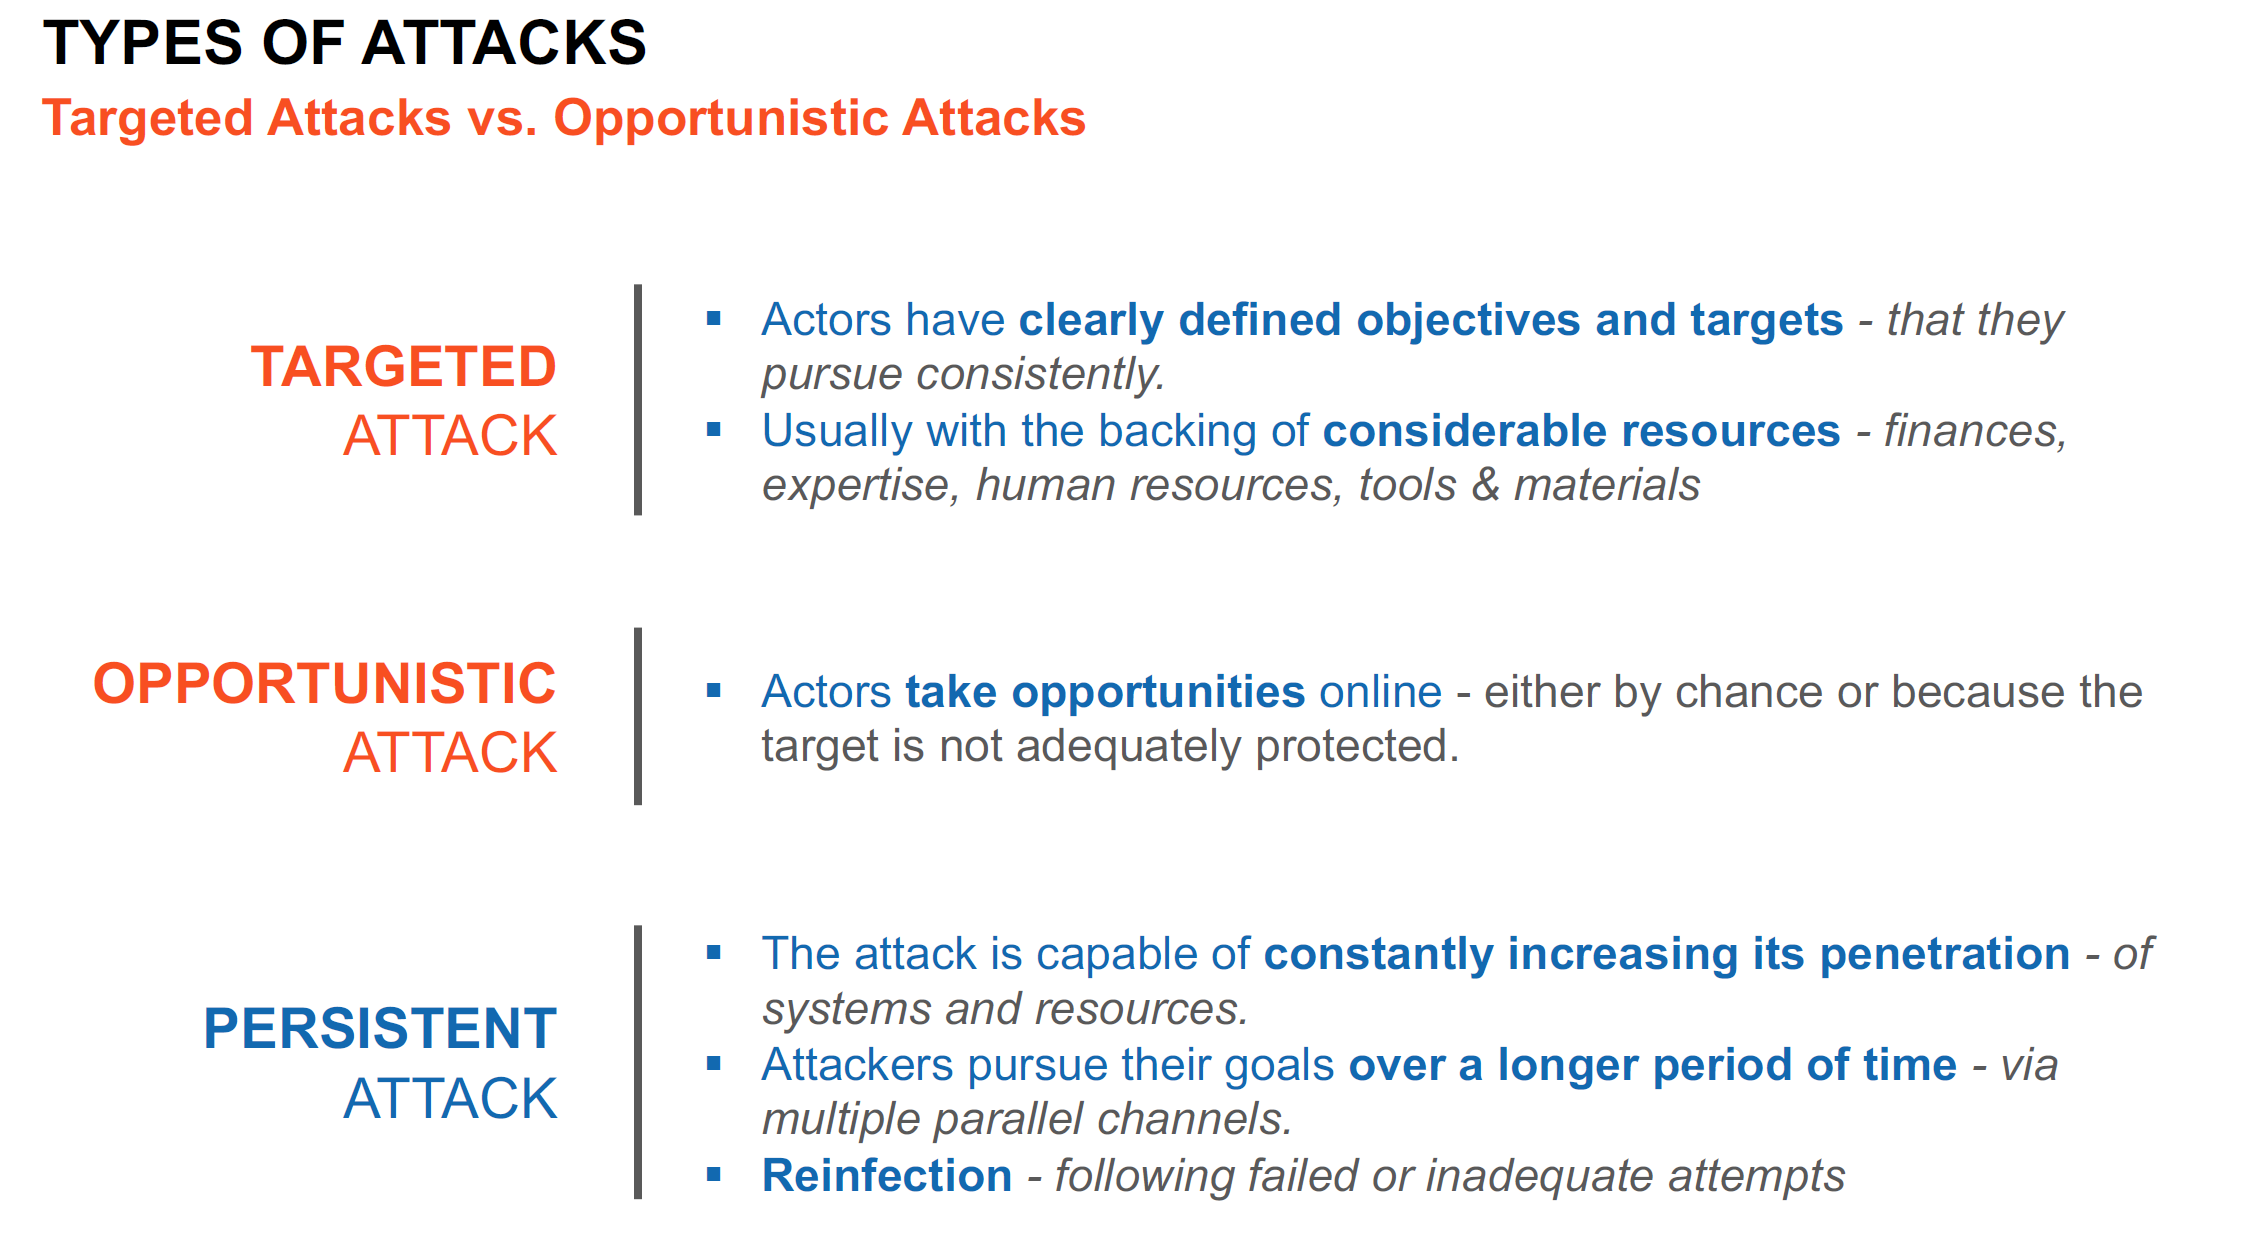
\includegraphics[width=\linewidth]{Figures/IDS_attack_types.PNG} 
\end{minipage}

\begin{minipage}{\linewidth}
    \centering      
    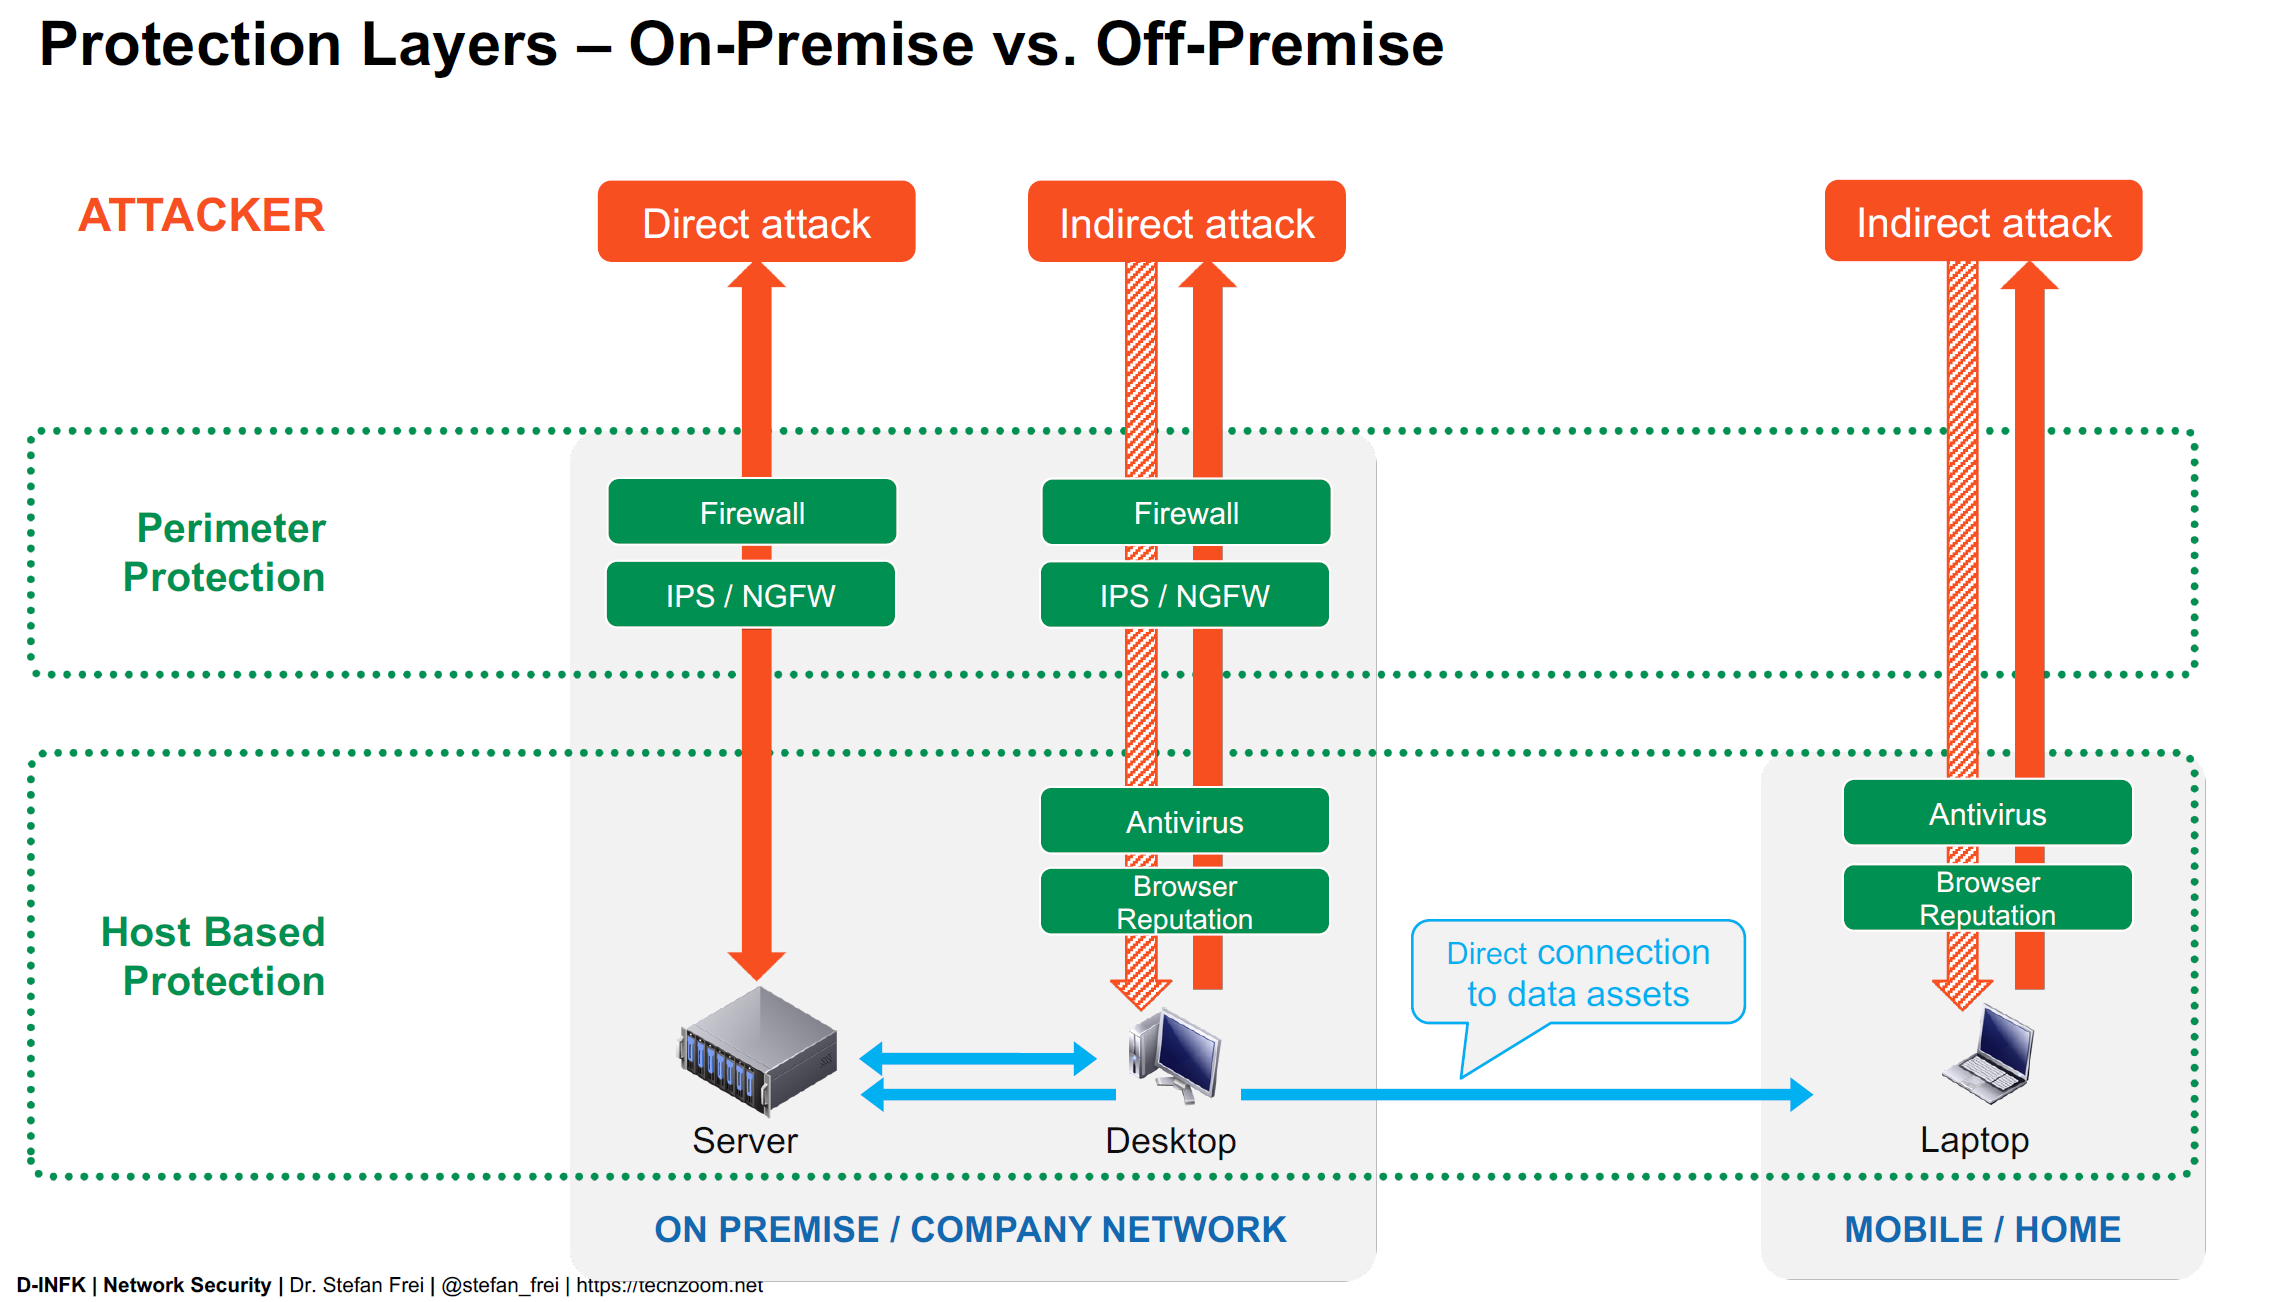
\includegraphics[width=\linewidth]{Figures/IDS_protection_layers.PNG} 
\end{minipage}

\begin{itemize}
	\item Direct attack: “server-side” exploits, the threat/exploit is executed remotely by the attacker against a vulnerable application and/or operating system
	\item Indirect attack: the threat/exploit is initiated by the vulnerable target. The attacker has little or no control over when the target user executes the threat.
\end{itemize}

\begin{minipage}{\linewidth}
    \centering      
    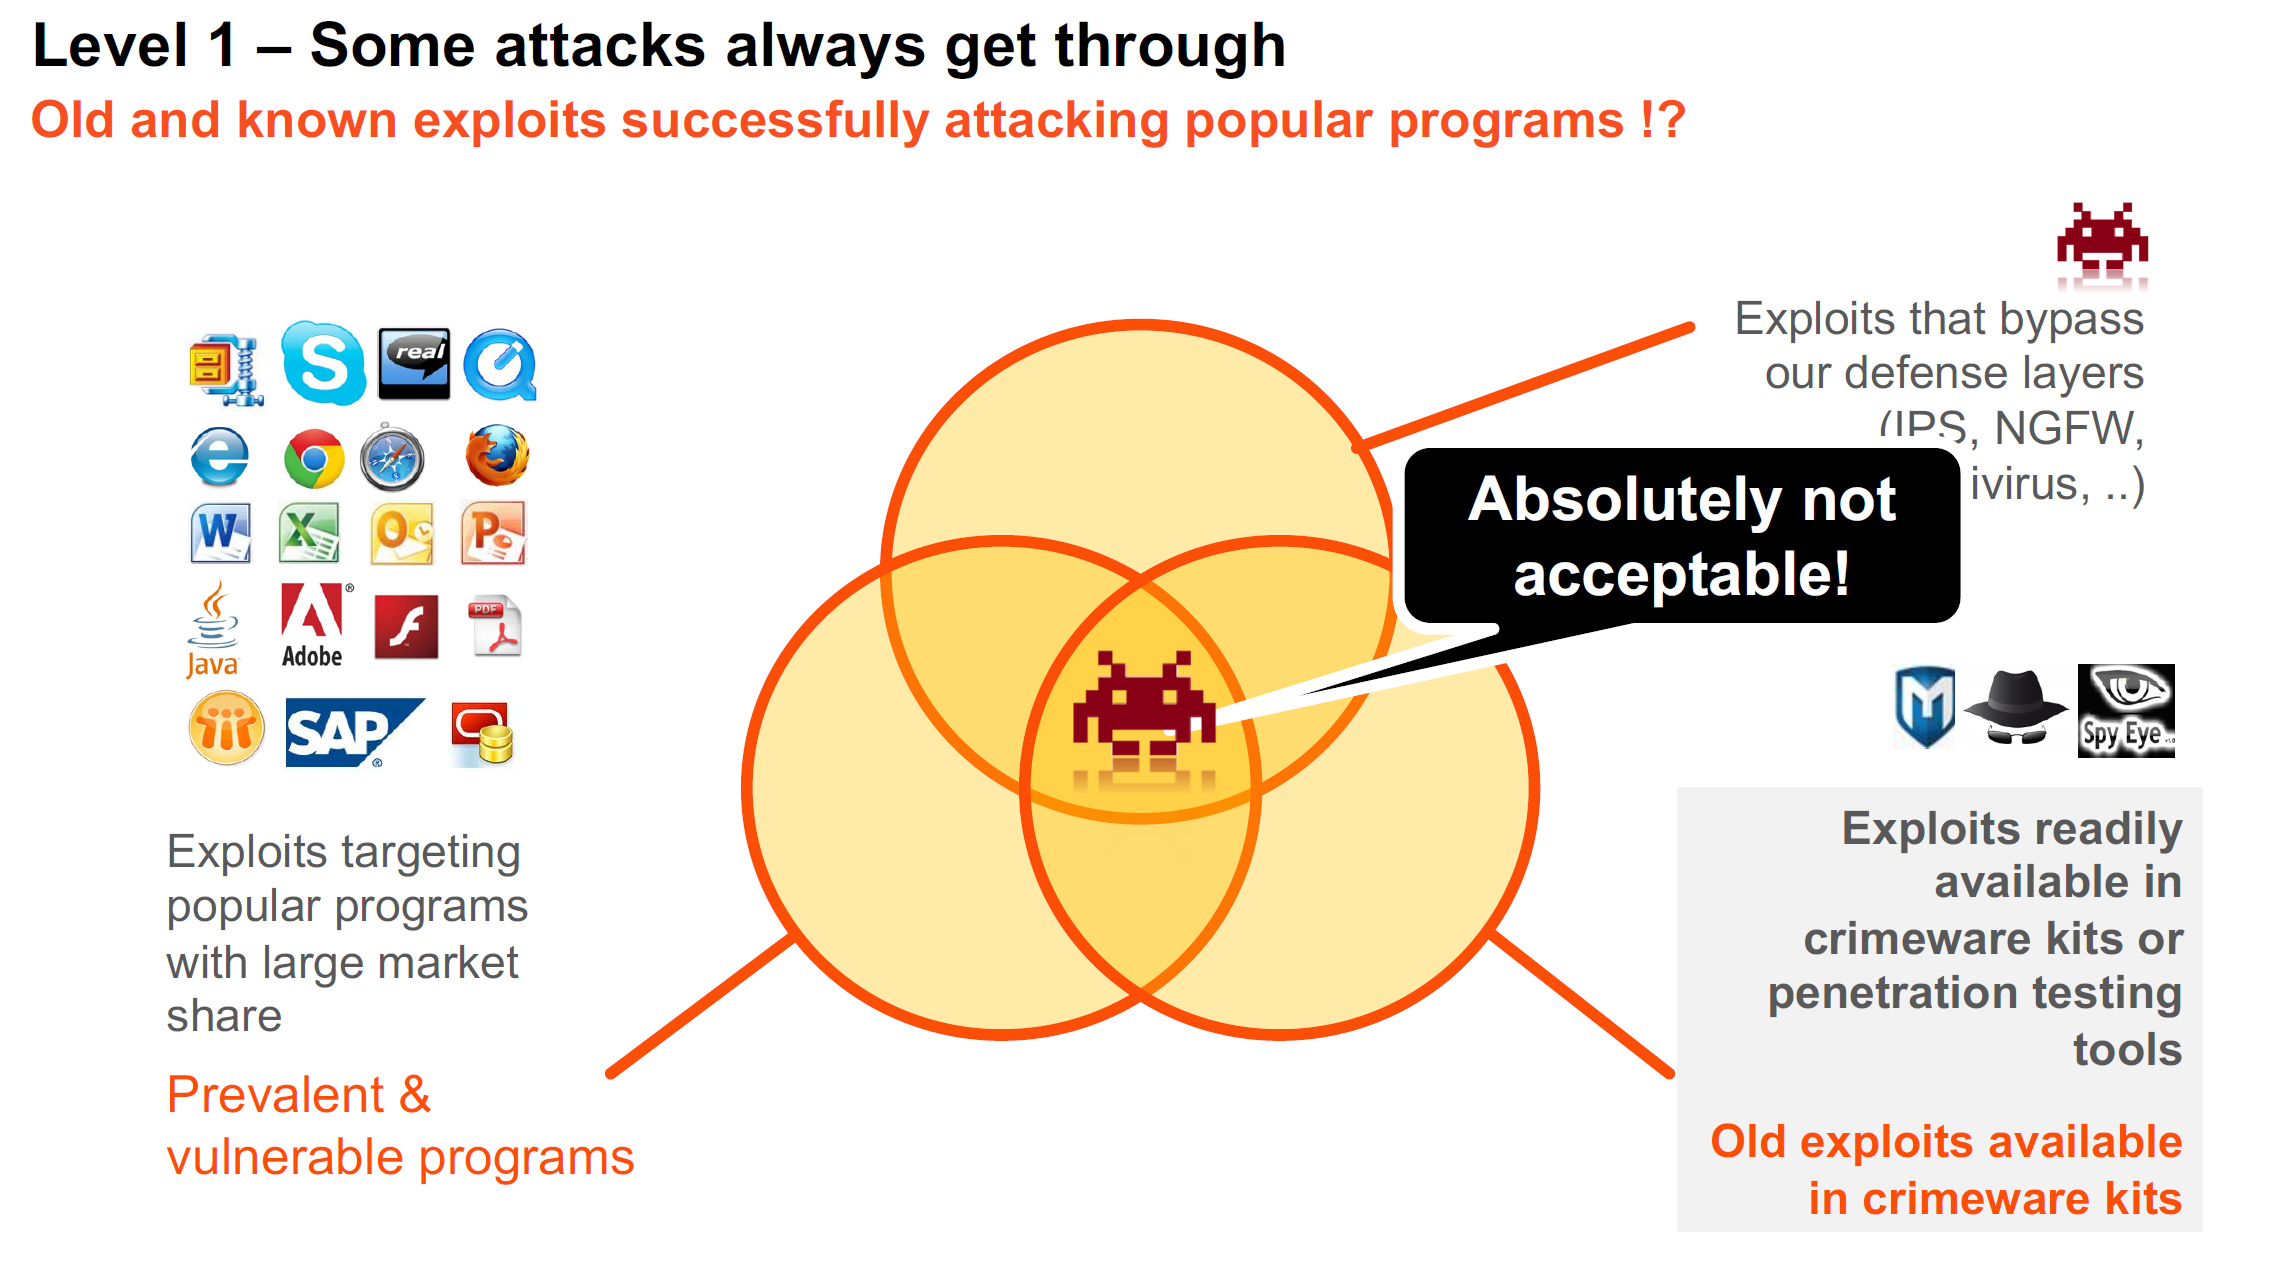
\includegraphics[width=\linewidth]{Figures/IDS_attack_model.PNG} 
\end{minipage}

\subsection{Botnets}

\paragraph{Basic components:}

\begin{itemize}
	\item Bots: devices under control of the attackers – often vulnerable hosts that have been
	infected with a malware.
	\item Command and Control infrastructure: often owned by the attackers, is it used to push
	commands to the bots.
\end{itemize}

\subsubsection{Mirai botnet}
\label{mirai_botnet}

Mirai mainly targeted IoT devices. IoT devices are a very interesting attack vector since there are lots of IoT devices (ca. 10 billion for 2019), they are configure-and-forget (owners don't update them and don't realize when they're compromised) and security is often lacking in IoT devices.\\
Mirai has been used mainly for Distributed Denial of Service attacks. DDoS is much harder to track and take down than a regular DoS. This allows the attacker to hide his identity behind the botnet. Additionally, a DDoS enables the attacker to have a virtually unlimited bandwidth for flood attacks.\\
Mirai infection technique:

\begin{enumerate}
	\item Scan: infected device scans network for open Telnet ports (send TCP SYN packets to random IPv4 addresses)
	\item Brute force: the bot tries to log in using 10 random user/pass combinations taken from
	a hardcoded list of 62. These represent default credentials of existing devices.
	\item Report: upon login success, the bot reports the target to a Report Server. It lists IP
	address, type of device (if available) and successful credentials.
	\item Infection: a Loader program gets a detail of the target from the Report Server, connects
	to Telnet and uploads the correct malware binary to the machine.
\end{enumerate}

Mirai is non-persistent: the binary is loaded into memory and immediately deleted from disk. Rebooting will remove the malware, but the device can still be reinfected. This makes detection and forensic analysis more difficult, especially for IoT devices.\\
Mirai infected devices were fingerprinted by the fact that Mirai generated probe packets had their sequence number equal to the IP of the scanned device. Probability of this happening is $\frac{1}{2^{32}}$.

\subsection{Stuxnet}

Stuxnet is the first (publicly know) cyberweapon - a complex malware, widely believed to have targeted uranium enrichment infrastructure in Iran. Stuxnet used various infection vectors such as WinCC machines, network shares, print spooler zero-day, removable drives (to jump airgaps). Stuxnet installed a driver, signed with a legitimate Realtek certificate. This driver intercepts I/O requests, making the files installed by the malware invisible. It also registers as a boot start service, acting as load point at reboots. This driver behaves very much like a legitimate Windows driver: this, and its legitimate Realtek signature, make it very hard to detect even for an experienced sysadmin. Stuxnet would survive manual inspection, OS updates and antivirus scans. This required legitimate certificates. Using fake certificates would have also been possible but surviving system updates would become harder. Hiding in plain sight is often a winning strategy. Stuxnet often injected itself into the privileged antivirus process to ease the infection. Depending on the antivirus, it alternatively ignored it and injected itself in a Windows system process. 

\section{Internet of Things (IoT)}
\label{iot}

\subsection{Common Ground}

\begin{itemize}
    \item Safety = protection against accidents (environment doesn't adapt to bypass safety measures).
    \item Security = protection against targeted attacks (adaptive attacker).
\end{itemize}
\\
The biggest challenge in cyber security is the misconception of risk. Humans perceive fire as risky. (Most) humans don't perceive their smart toaster as a risk, although it is. People need highly visible incidents before they act. We no longer live in a complicated system but in a complex adaptive system \textbf{CAS}:

\subsection{IoT (and IIOT, ICS, SCADA, OT\&IT)}

\begin{itemize}
	\item \textbf{Information Technology (IT):} The entire spectrum of technologies for information processing, including software, hardware, communications technologies and related services. Generally does not include embedded devices.
	\item \textbf{Operational Technology (OT):} Hardware and software that detects or causes a change through the direct monitoring and/or control of physical devices, processes and events in the enterprise.
	\item \textbf{Industrial Control Systems (ICS):} Systems that are used to monitor and control industrial processes focused on automation, computerized monitoring and control of physical industrial processes (e.g. oil refining). Typically considered to be mission-critical applications with a high-availability requirement.
	\item \textbf{Internet of Things (IOT):} High level concept of a global network of “smart” physical objects of various kinds (wearables, smart toaster,...)\
	\item \textbf{Industrial Internet of Things (IIOT):} Subset of IoT specific to industry (e.g. advanced field sensors)
	\item \textbf{Critical Infrastructure (CI):} Critical infrastructure refers to processes, facilities, technologies, networks and systems (including IIOT and ICS) that control and manage essential services. Disruptions of critical infrastructure could result in catastrophic consequences.
\end{itemize}
\\
Our world is quickly changing in an irreversible move towards IT/OT convergence. Extending security models to include the OT domain introduces many challenges: conventional IT security thinking hasn't reached (I)OT industry yet, OT devices must not be assumed to be ‘just another end point’.

\paragraph{Key Differences between IT and OT:}
\textbf{OT: availability \& integrity}
\begin{itemize}
    \item at edge of the network
    \item long life cycle
    \item slow response to threats
    \item Limited data capacity and computing power
    \item Safety Operations is critical
\end{itemize}
\\
\textbf{IT: Confidentiality} (integrity, availability):
\begin{itemize}
    \item at the center of the network (consumer at edge)
    \item short life cycle
    \item rapid response to threats
    \item High data capacity and computing power
    \item Few safety critical operations
\end{itemize}

\subsection{IOT	Attack Surface}

\paragraph{Example 1: STRAVA - the nr. 1 app for runners and cyclists}
Data about exercise routes shared online by soldiers can be used to pinpoint overseas facilities, and individuals. Location of military bases and individual identities exposed

\paragraph{Example 2: Ingoring Known Security Best Practice}
Hacked jeep

\paragraph{Example 3: Modern Airplanes - Legacy Communications}

\paragraph{Attack Surface}
IOT connects innumerable everyday devices and systems. Previously closed systems are opened up to remote access and control. This opens up a large attack surface:

\begin{itemize}
	\item Device: insecure software, lacking update mechanism
	\item Communication: insecure communication, weak or no cryptography, lack of authentication
	\item Backend services: Central control, erosion of privacy, data breaches
\end{itemize}

Further, user perception of risks in cyber security is usually wrong: most users perceive their PC as exposed to malware and fear getting malware but think their smart TV, smart toaster, smart everything are great and don't pose any risks. In reality, the opposite is the case: PC security is rather sophisticated (hardened over 20 years) and we have frequent security updates (e.g.finding a vulnerability in Win10 is hard). But IoT devices ran in isolation for years and only recently became connected. They are designed for high availability and safety, \textit{not} security. Further, IoT devices rarely get security updates. However, the threat environment only gets worse over time, thus we rapidly create a huge future liability with devices lacking an automated and robust protection functionality.\\
To make matters worse:

\paragraph{Attacking Embedded Devices:}
\begin{itemize}
    \item OSINT: Open source intelligence, retrieve firmware from vendor website. Get devices from e-bay.
    \item Access Debug Interfaces: Retrieve firmware, configurations, secrets.
    \item IoT devices are mass produced, if an attack is built for one of these devices it can be replicated across all same devices.
    \item Root Access to the device through default accounts or secrets, certificates, device fleet passwords.
    \item We rapidly create a huge future liability with devices lacking automated and robust update functionality.
\end{itemize}

\begin{itemize}
	\item IoT devices typically have a much longer lifetime (1-20+ years) than phones/PCs. That's a long time: vendor could go bankrupt. Solutions: Code escrow (copy source code at trusted third party), open source software
	\item Certification vs. Security: operation critical devices (e.g. flight management system) need certification. However, digital products constantly require security updates which invalidates the certificate. Thus, we need to re-certificate after every patch. BUT: Certification timeline is outpaced by cyber security.
	\subitem \textit{You're doomed if you patch - you're doomed if you don't.}
\end{itemize}

\subsection{Possible approaches to make things better}

IOT security is part of a complex and evolving ecosystem of diverse domains. Technology based security solutions have to complement other domains to achieve the desired security level.

\begin{itemize}
	\item \textbf{enforce some minimal security standards and testing for IoT devices}
	\item Design systems with redundancy and resiliency.
	\item Active management of vulnerabilities (coordinated disclosure, bug bounty)
	\item Robust and scalable process to deploy security updates timely and efficiently - on any connected device
	\item Industry-wide systematic security and integrity testing of all critical components
\end{itemize}


\subsection{TRENDnet Security Breach}

IP cameras by Trendnet had vulnerability that allowed attackers to view live video stream of any camera. The root directory of the camera’s server had, next to the management directory, another script called mjpg.cgi This script, accessible at \texttt{https://IP\_ADDR/anony/mjpg.cgi}, streamed the captured video in real-time without the need of any authentication. Shodan (\href{https://www.shodan.io/}{shodan.io}) was used by attackers to find IPs with that camera behind.

\section{DNS Security}

The Internet is a critical infrastructure, yet its operation depends on the fundamentally insecure DNS. DNS provides a mapping of names to resources of several types. However, DNS, as a robust key protocol of the Internet, is also a formidable attack vector for cyber criminals:

\begin{itemize}
	\item Manipulating the DNS mapping allows an attacker to redirect connections to malicious server, facilitate MitM attacks and launch DoS attacks.
	\item DNS helps building hidden channels (tunneling)
	\item is abused for powerful denial of service attacks
	\item is abused for various impersonation attacks
	\item used to setup services that are hard to hunt-down or shut-down (Botnets, Fast- & Domain Flux)
\end{itemize}

\subsection{Domain Name System (DNS)}
DNS is a globally distributed, loosely coupled, scalable, reliable and dynamic database. DNS data is maintained locally and retrievable globally, no single computer has all DNS data. 
DNS uses hierarchical namespaces to scale: tree structure down from root level ".", to top-level domains (TLD, e.g. .com) to second-level domains (SLD, e.g. google.com). A fully qualified domain name (FQDN) for example is mail.ethz.ch. The hierarchy descends from right to left. Domains are namespaces: everything below .com is the \textit{com} domain, everything below .ibm.com. is the \textit{ibm.com} domain.

\begin{minipage}{\linewidth}
    \centering      
    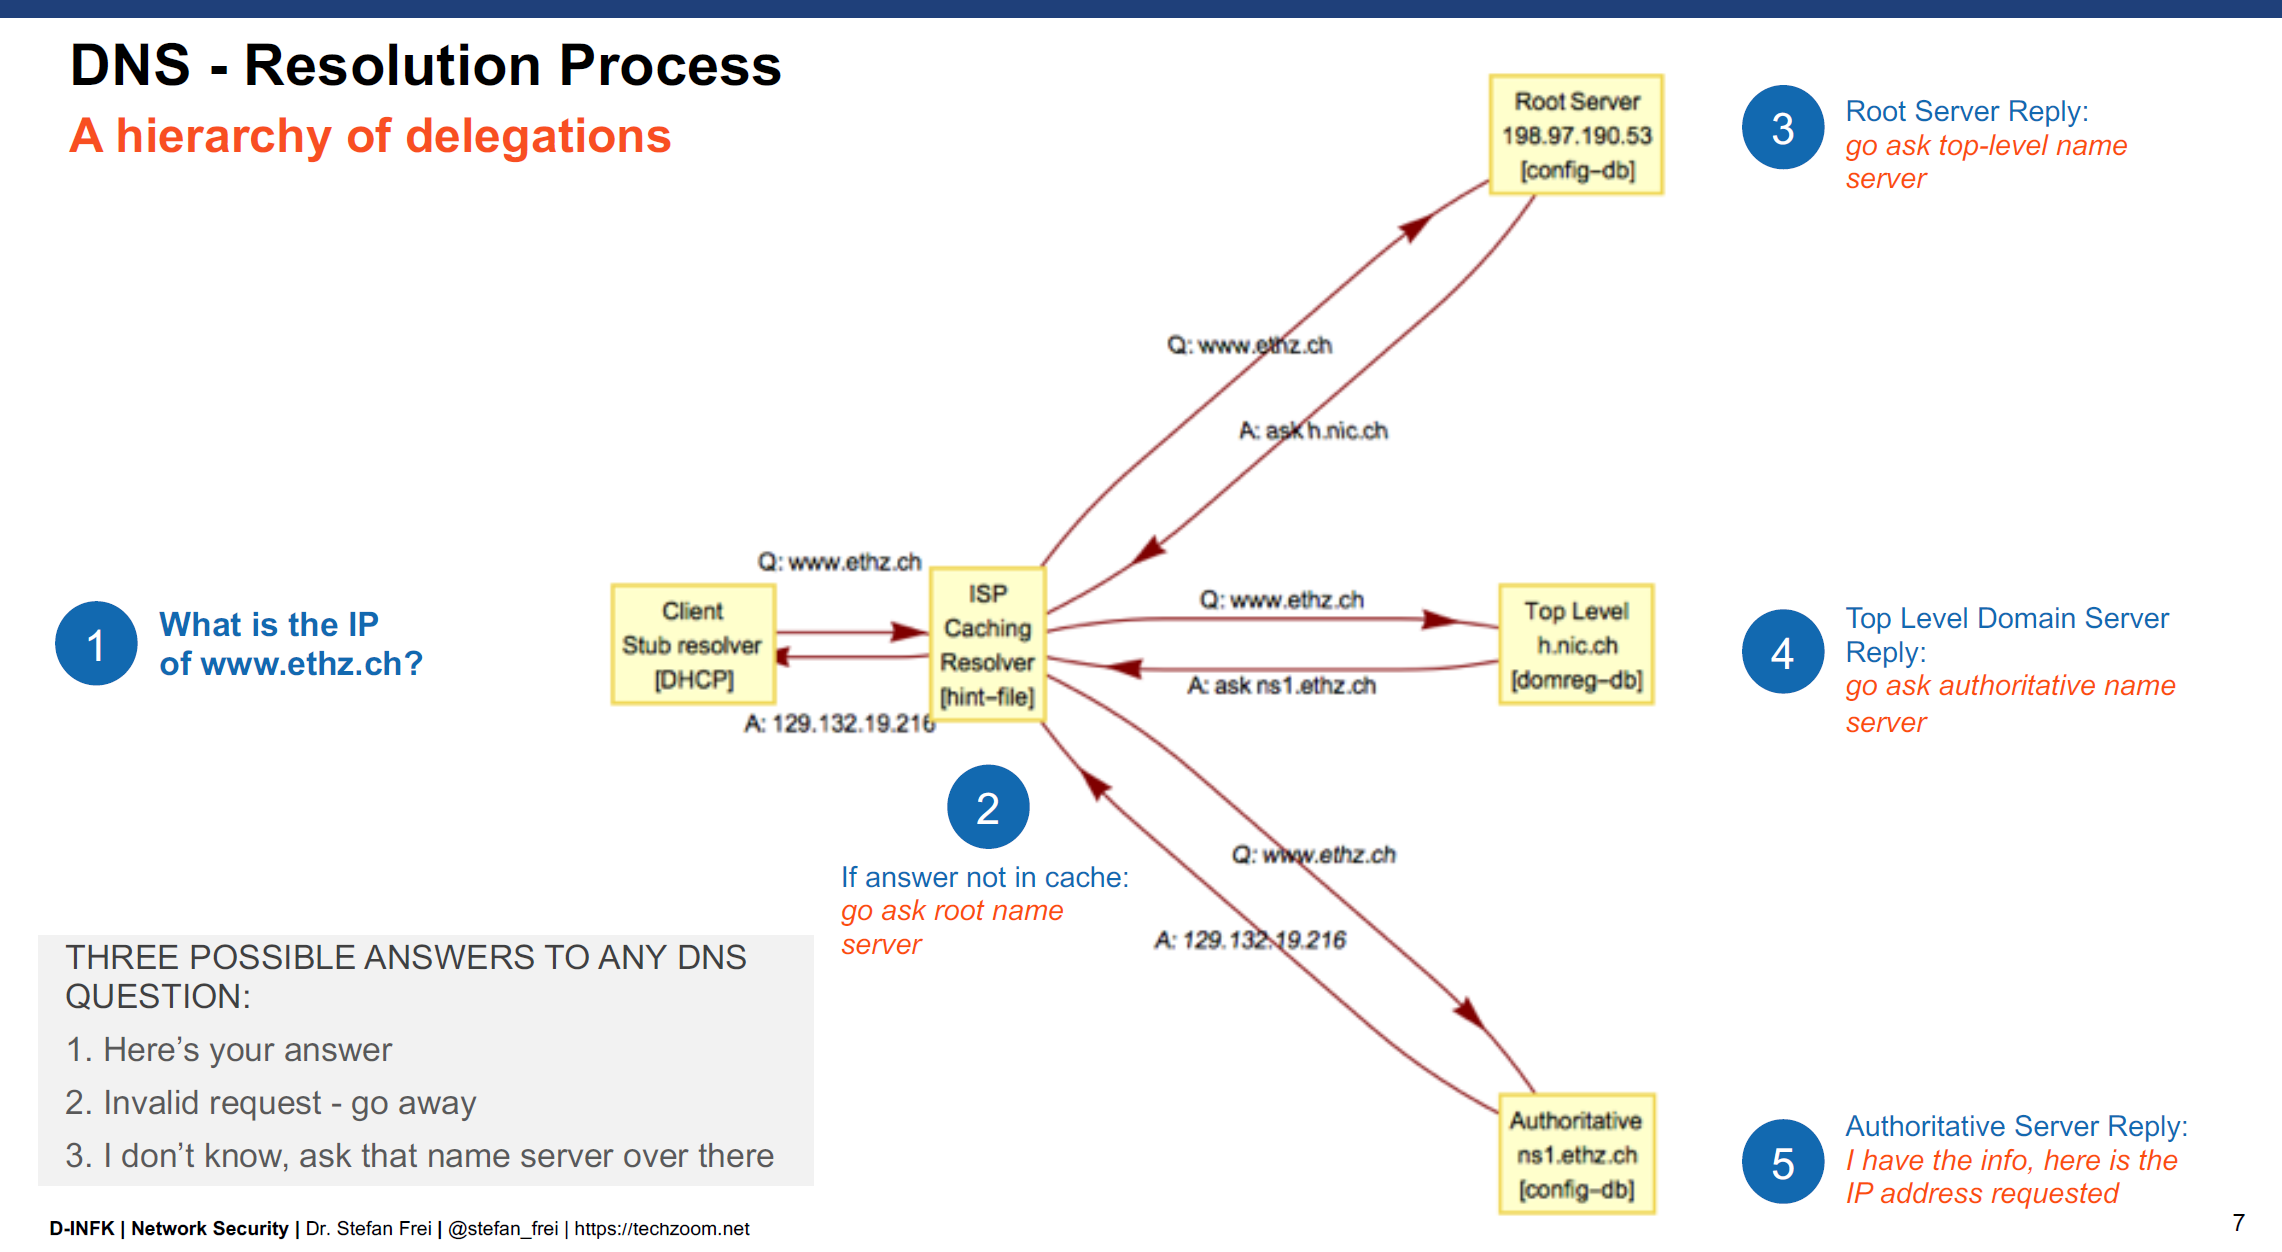
\includegraphics[width=\linewidth]{Figures/DNS_resolution.PNG} 
\end{minipage}

\subsection{DNS Protocol Features}
The DNS protocol was designed with a mechanism to protect against forged responses. The first two bytes in the message form a transaction ID (txid) that must be the same in the query and response.

\begin{itemize}
	\item Protocol: simple client-server protocol, operating on TCP/UDP port 53. No encryption, authentication nor integrity built into original protocol.
	\item Name server: Servers that map names to objects (= resource records RR). Authoritative: server is authoritative for a specific zone. Caching/Resolver: server resolves domains recursively, caches results.
	\item Client sends query and random txid, dnsserver responds with query, txid, response.
	\item Resolver: Client side of DNS resolution, responsible for initiating and sequencing the queries that ultimately lead to a full resolution. Stub resolver: piece of software running on a client that sends recursive DNS requests to a recursive resolver. Recursive resolver: processes DNS resolution iteratively to	provide full answer: it contacts all the different servers at the different domain levels to get the final answer.
\end{itemize}

\begin{minipage}{\linewidth}
    \centering      
    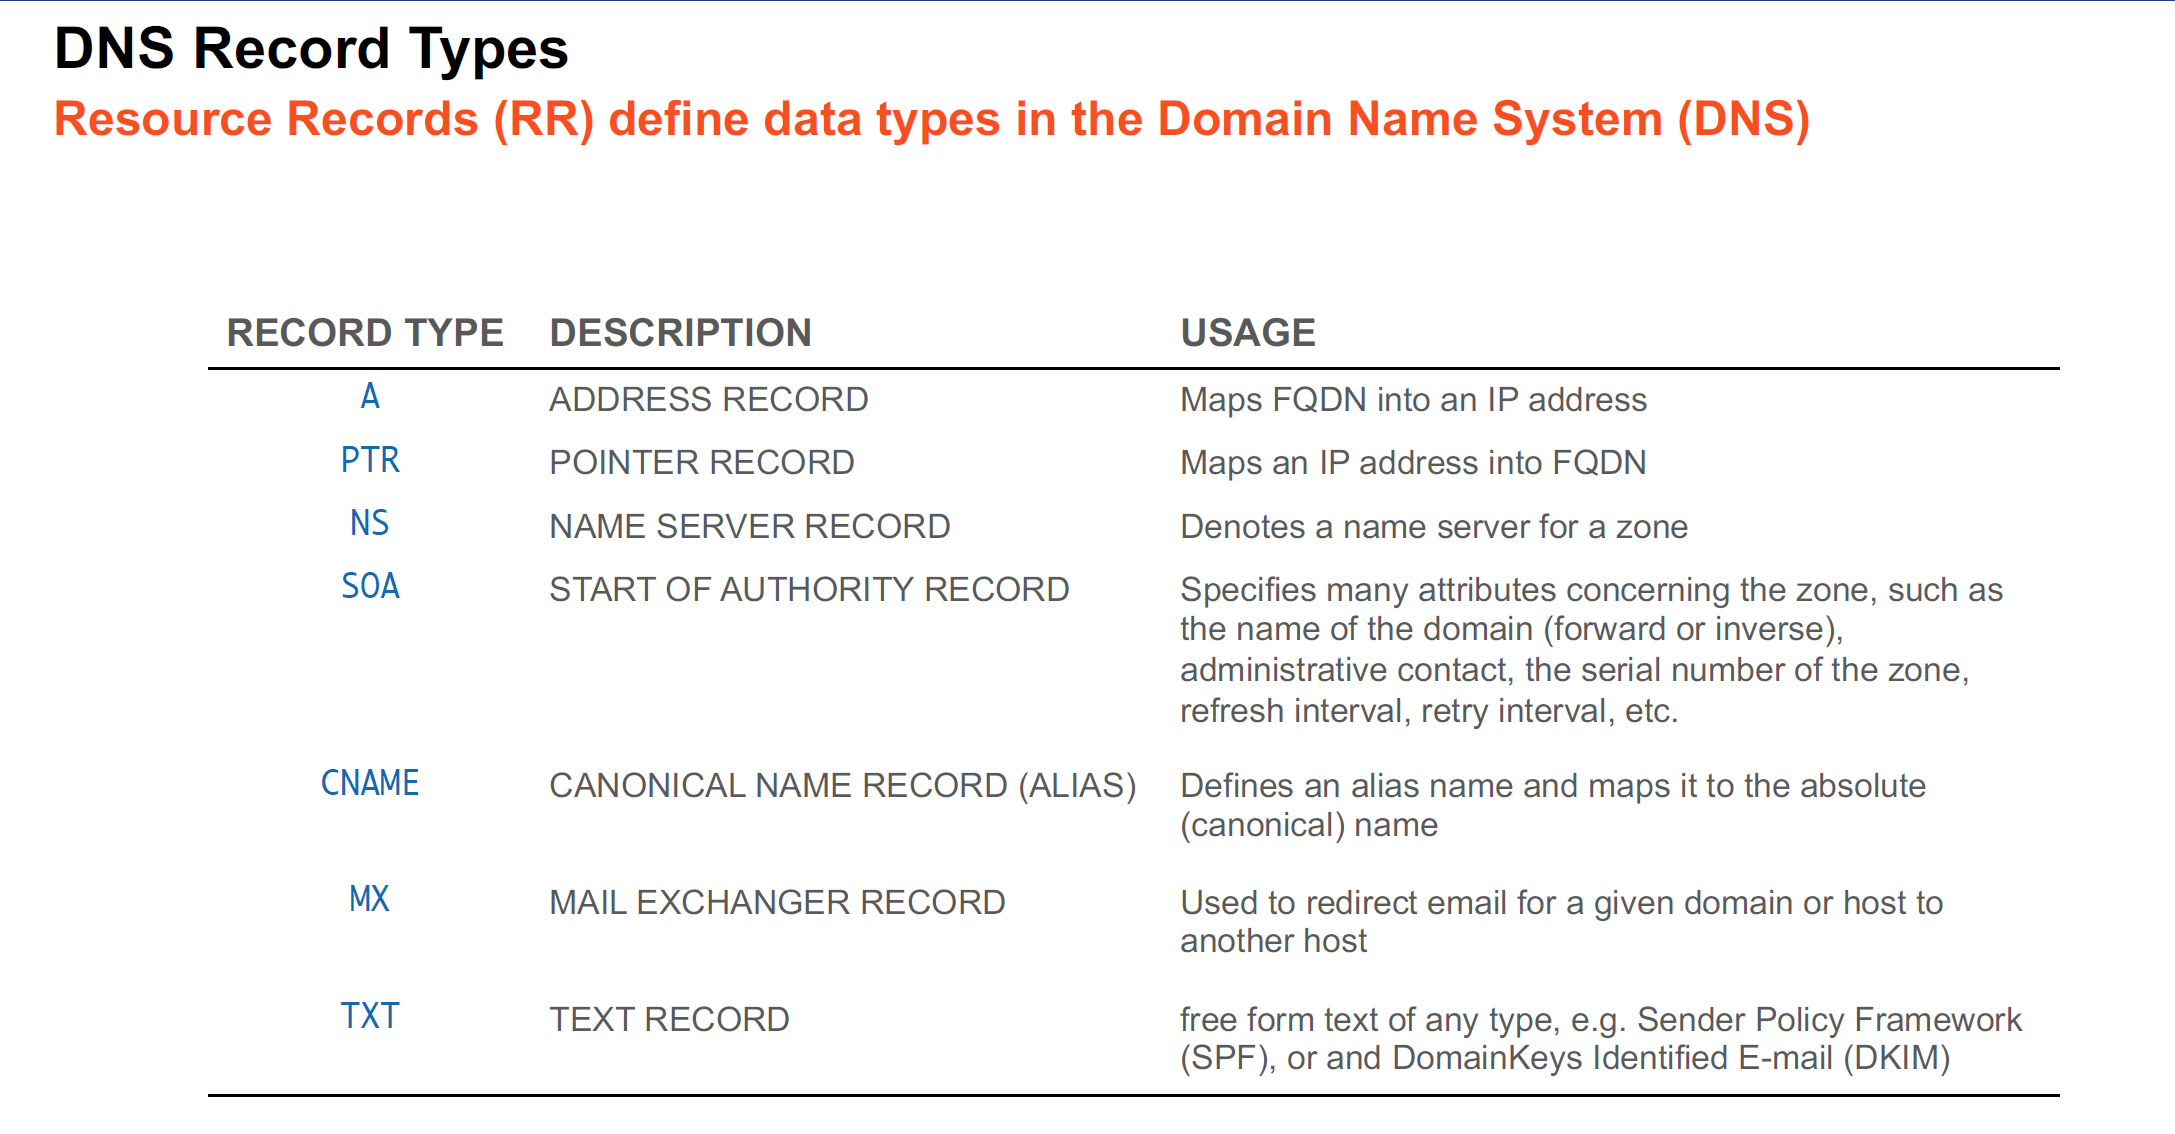
\includegraphics[width=\linewidth]{Figures/DNS_record_types.PNG} 
\end{minipage}

\paragraph{DNS Caching:}
We want to decrease lookup latency and network traffic. Each DNS response has a TTL. Caching resolvers will redo a recursive lookup once the TTL for a cached response has expired. A shorter TTL leads to shorter living cache entries, leading to faster refreshes for end users in case of an update. However, this means that there will be more load on the DNS servers for doing the recursive lookup again.

\paragraph{Attack Patterns:}
Insert tampered information into DNS server or resolution process. Control DNS of all clients served by name server/resolver

\begin{minipage}{\linewidth}
    \centering      
    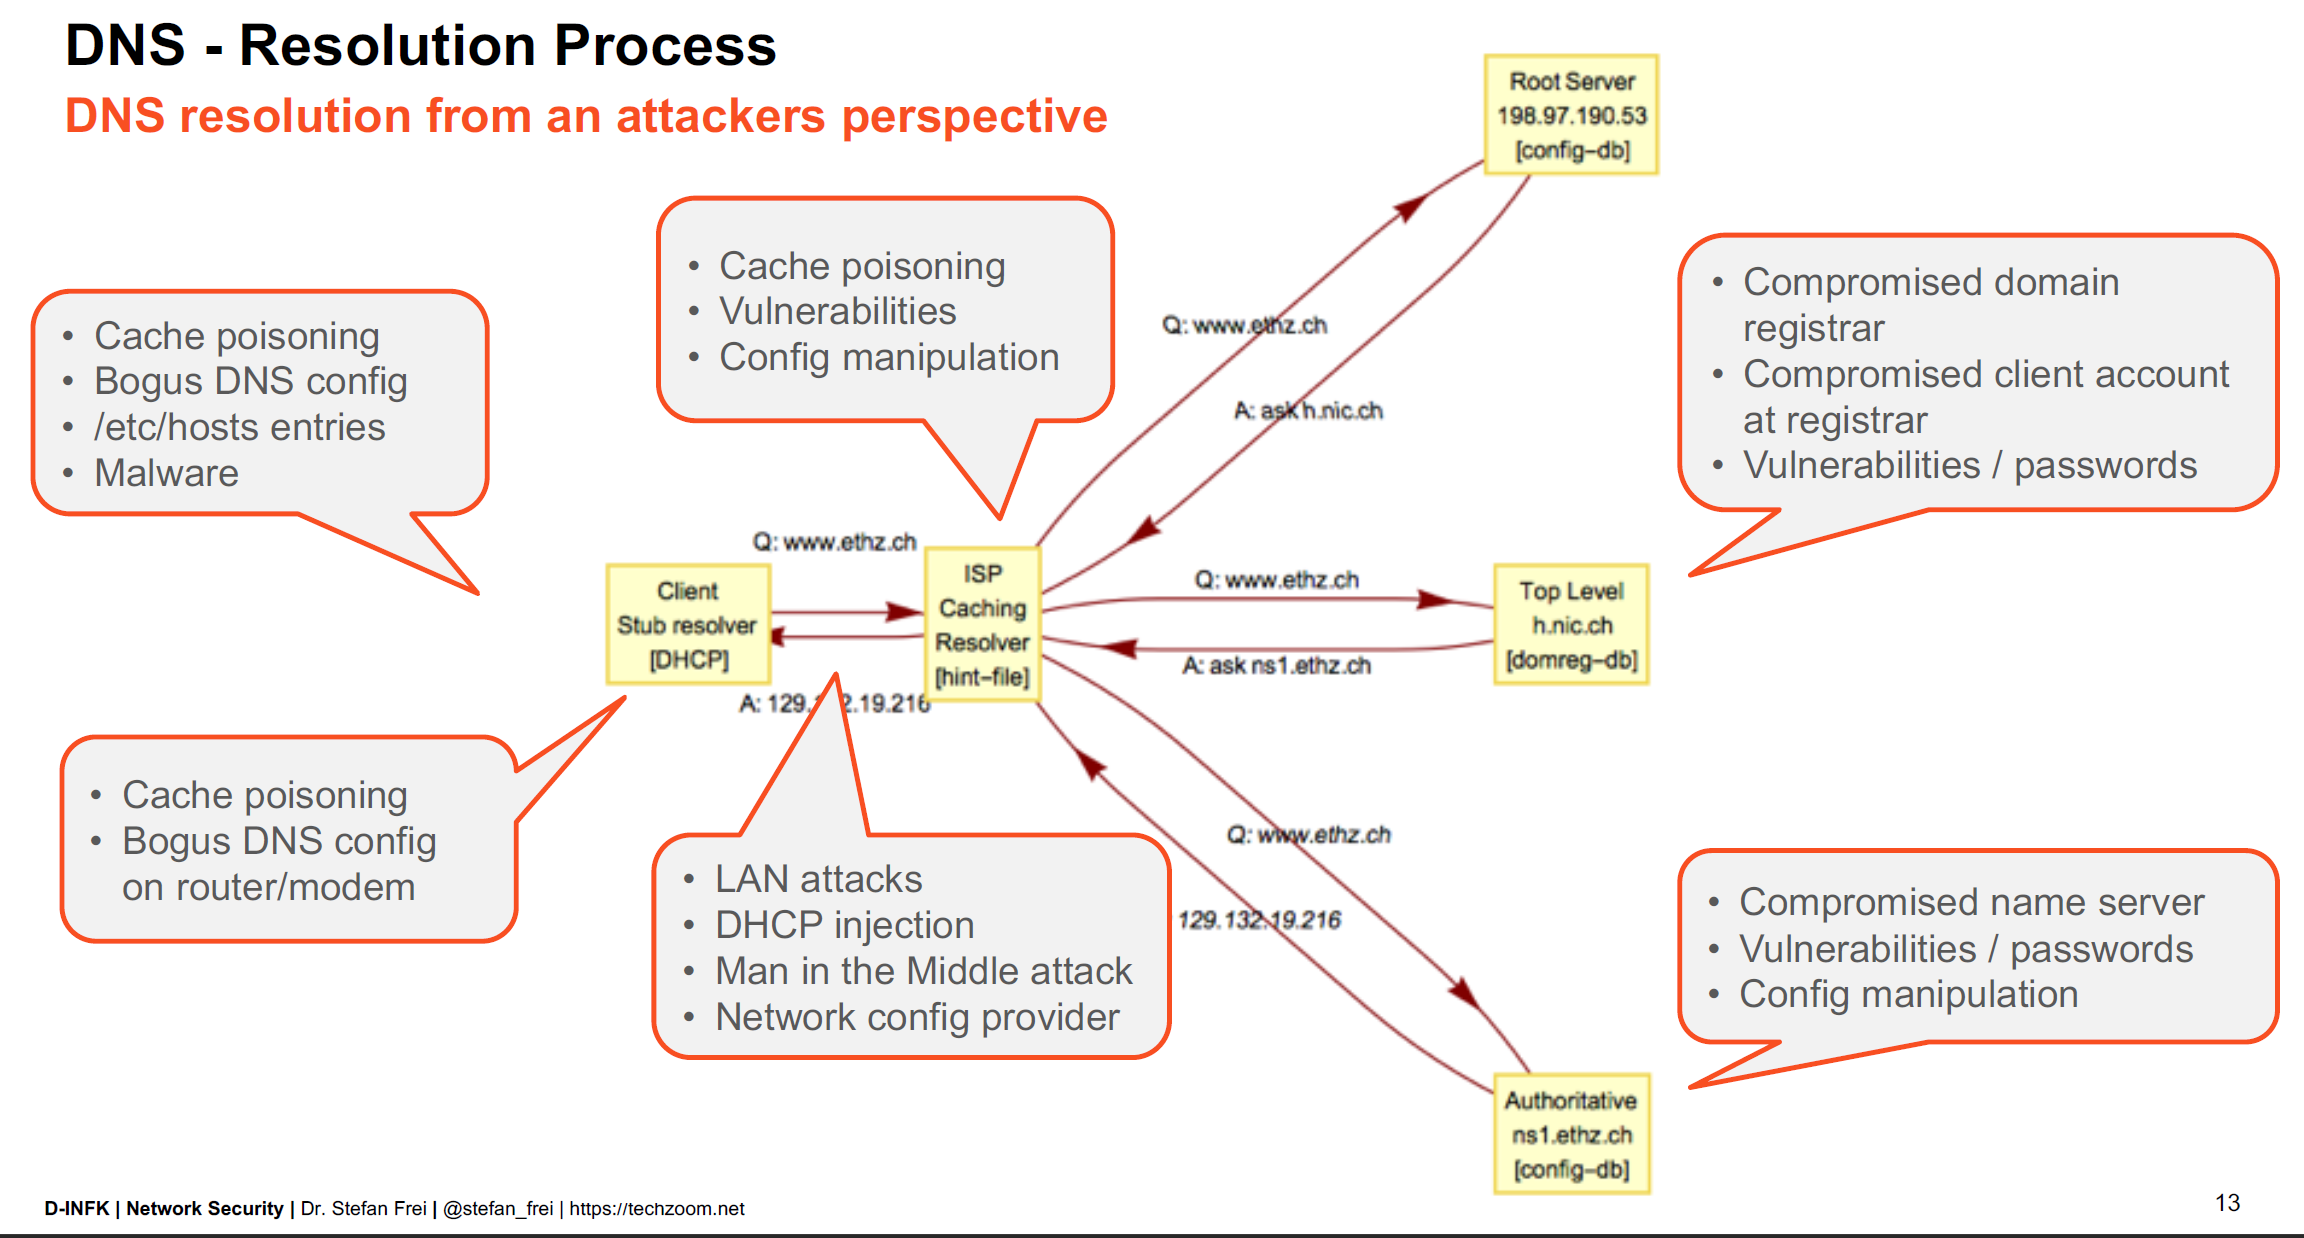
\includegraphics[width=\linewidth]{Figures/DNS_attacker_perspective.PNG} 
\end{minipage}

\begin{minipage}{\linewidth}
    \centering      
    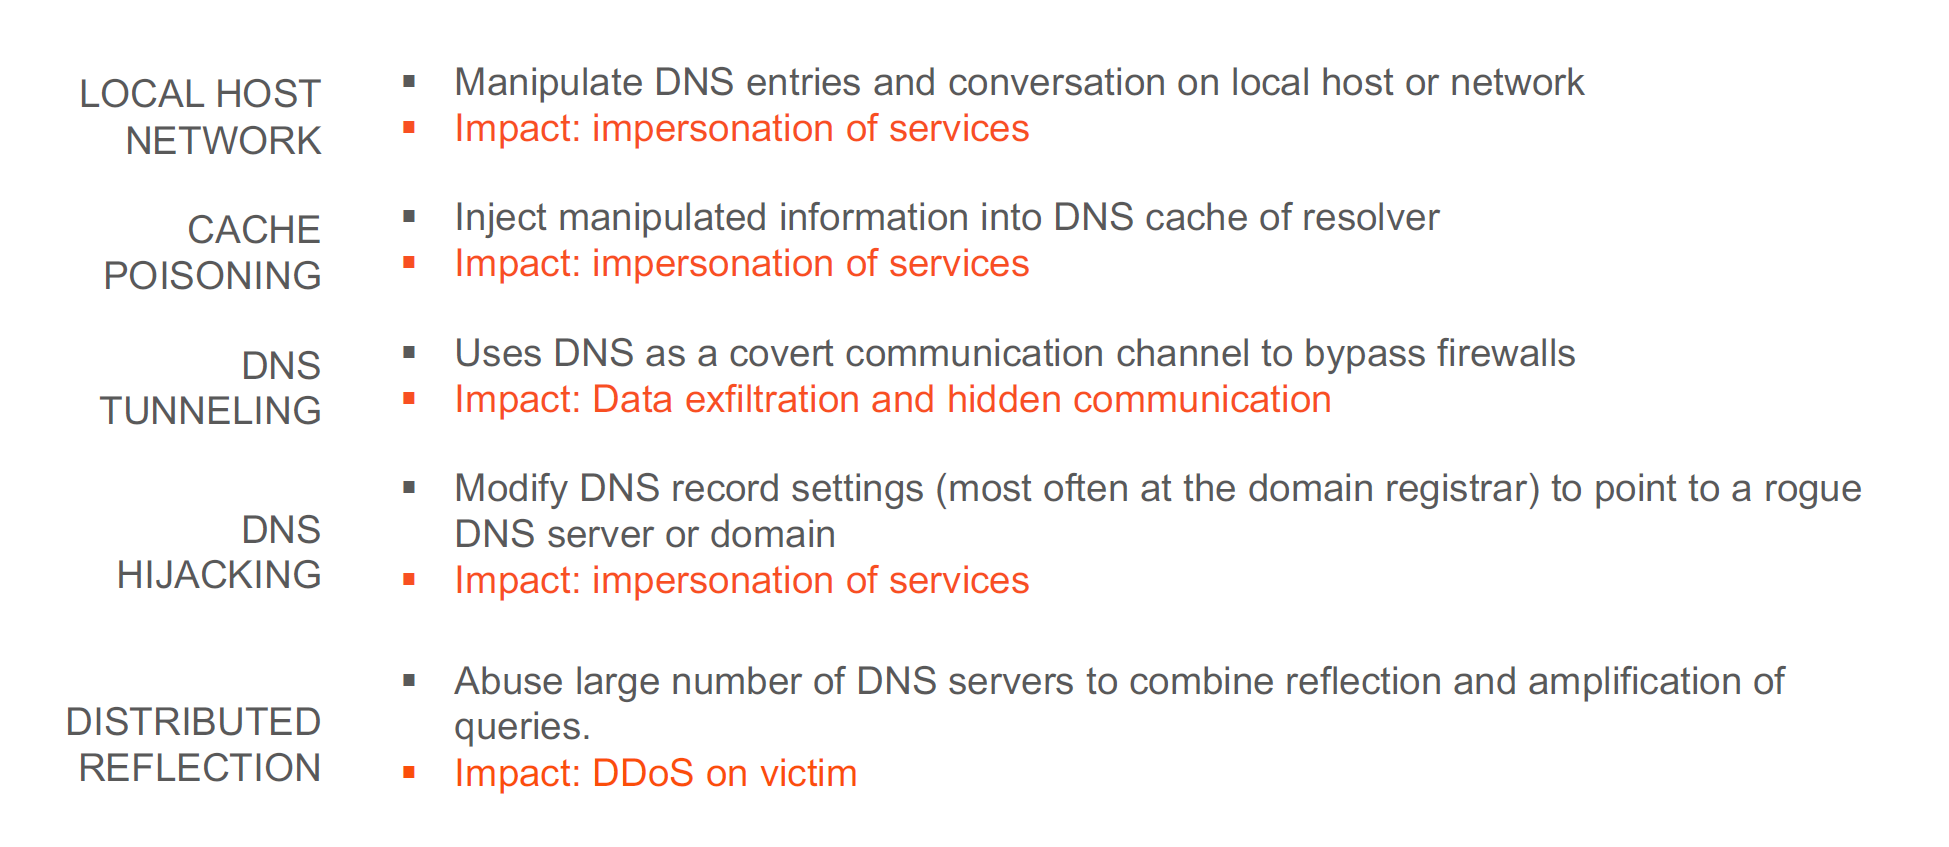
\includegraphics[width=\linewidth]{Figures/DNS_common_attacks.PNG} 
\end{minipage}

\subsubsection{Root servers}

\paragraph{DNS Root Zone:}
DNS root name servers are the key to the Internet kingdom: the DNS root zone is served by 13 root server clusters which are authoritative for queries for the top level domains. Every name resolution in the Internet either starts with a query to a root server, or, uses information that was once obtained from a root server. DNS root name servers have the official names a.root-servers.net to m.root-servers.net. They only resolve the IP addresses for the top-level name servers (TLD). The bandwidth available at RSS (Root Server System) is significant but no immune to DoS. Try to vary hardware in RSS to limit effects of a vulnerability.

\paragraph{Top-Level name servers}
A domain name registrar is an organization that manages the reservation of second-level Internet domain names (SLD) below a given top-level domain (TLD). A domain name registrar must be accredited by a top-level domain registry and/or a country code top-level domain (ccTLD) registry. Based on the domain registration database, the top-level name server points resolvers to the authoritative name server of the SLD.

\paragraph{Authoritative Domain Server}
The authoritative name server for a second-level domain is managed by private entities or on behalf of private entities that have registered a domain name. The authoritative name server has all records for a zone configured and can provide the final / authoritative information.

\subsection{Cache Poisoning}
\begin{minipage}{\linewidth}
    \centering      
    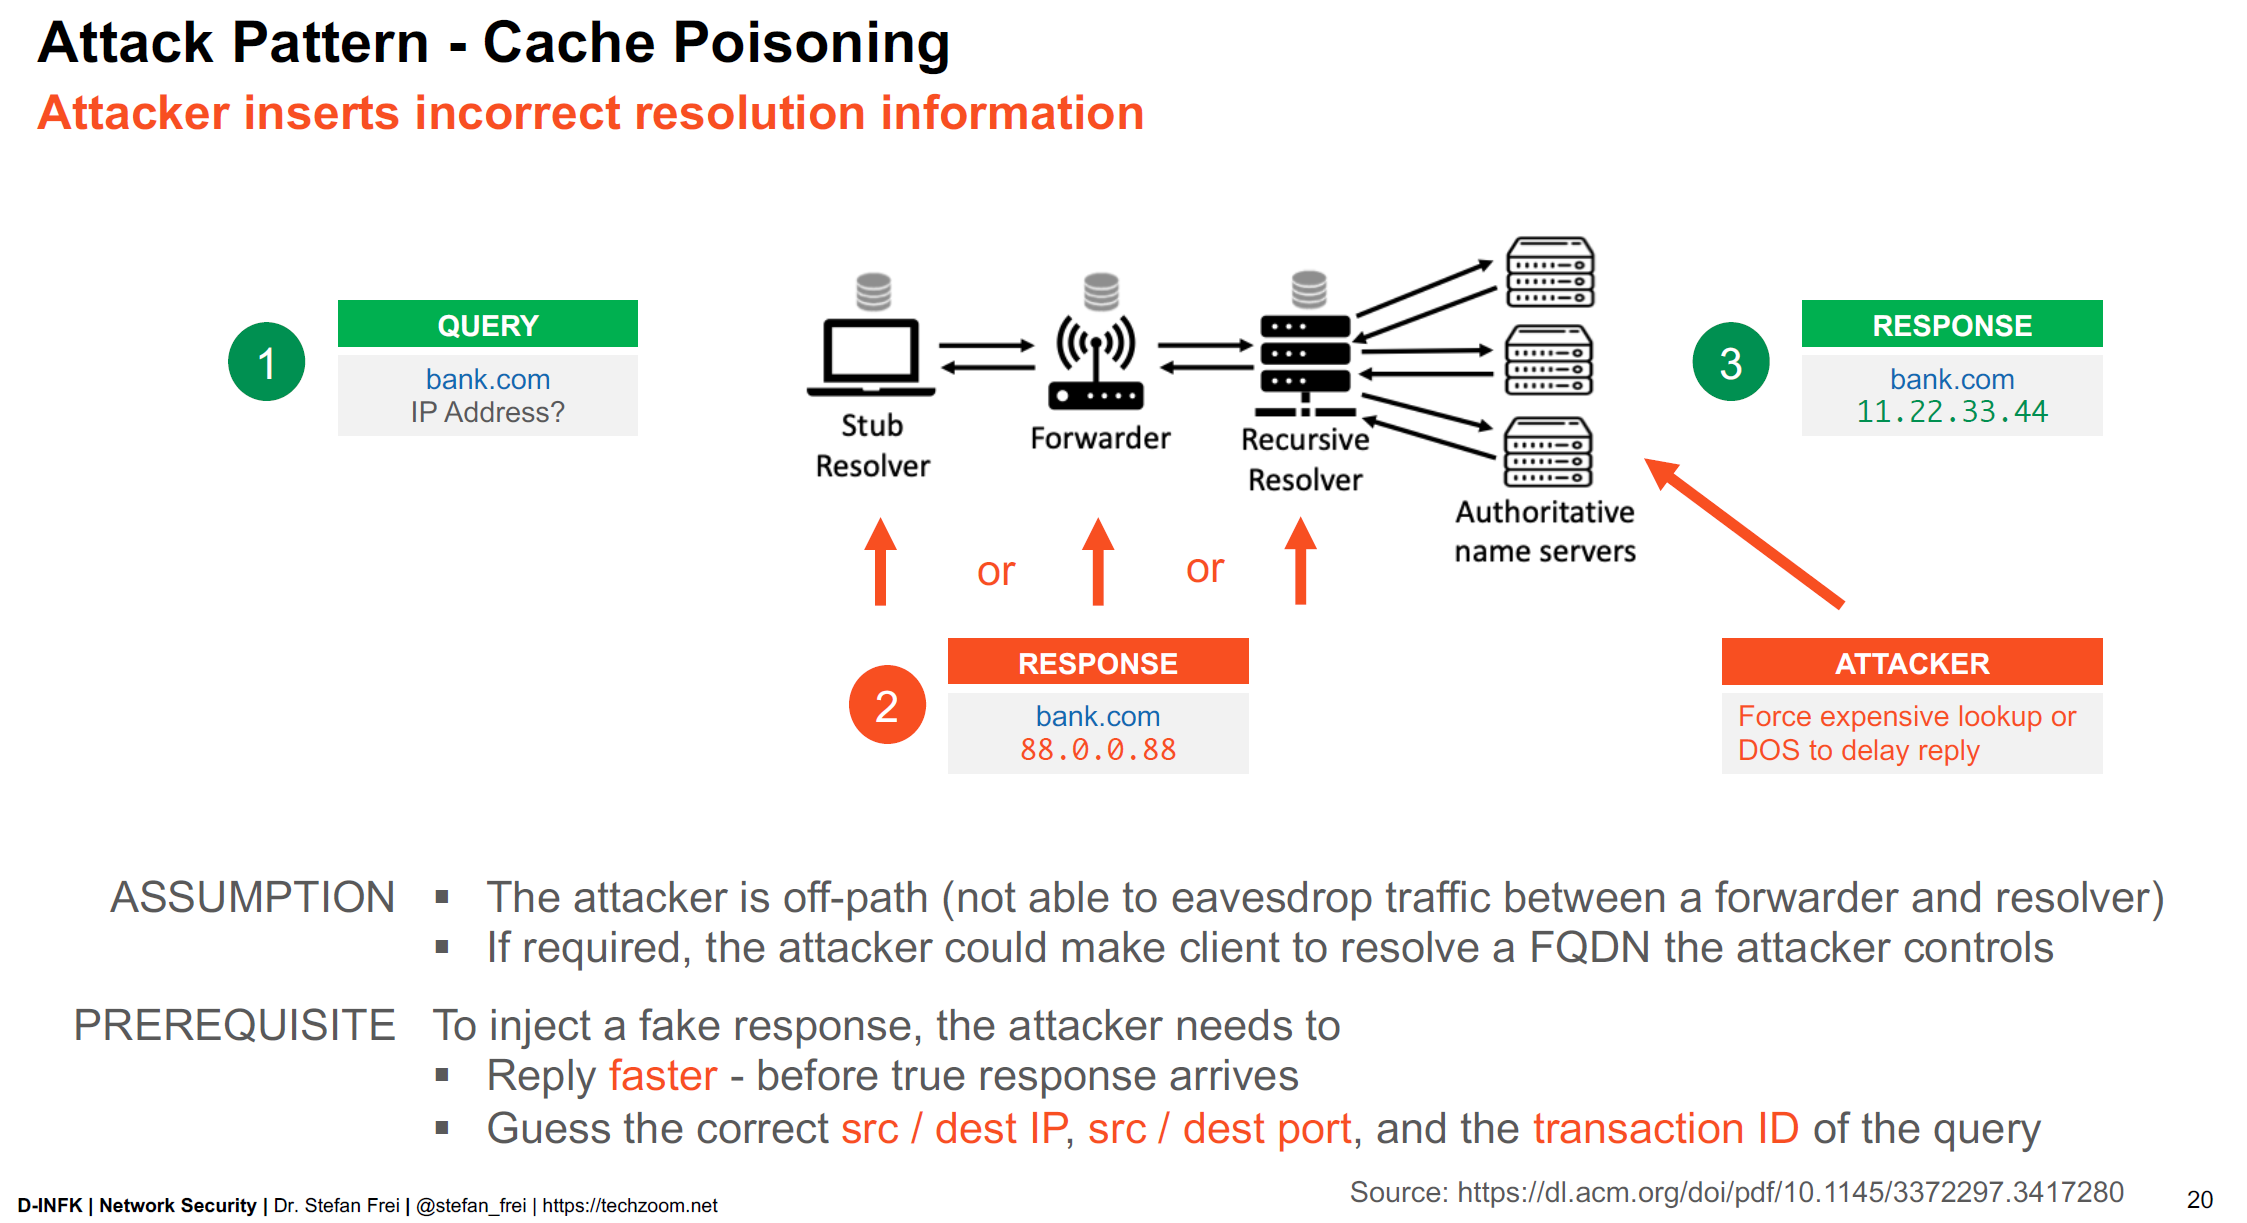
\includegraphics[width=\linewidth]{Figures/DNS_cache_poisoning.PNG} 
\end{minipage}

\begin{minipage}{\linewidth}
    \centering      
    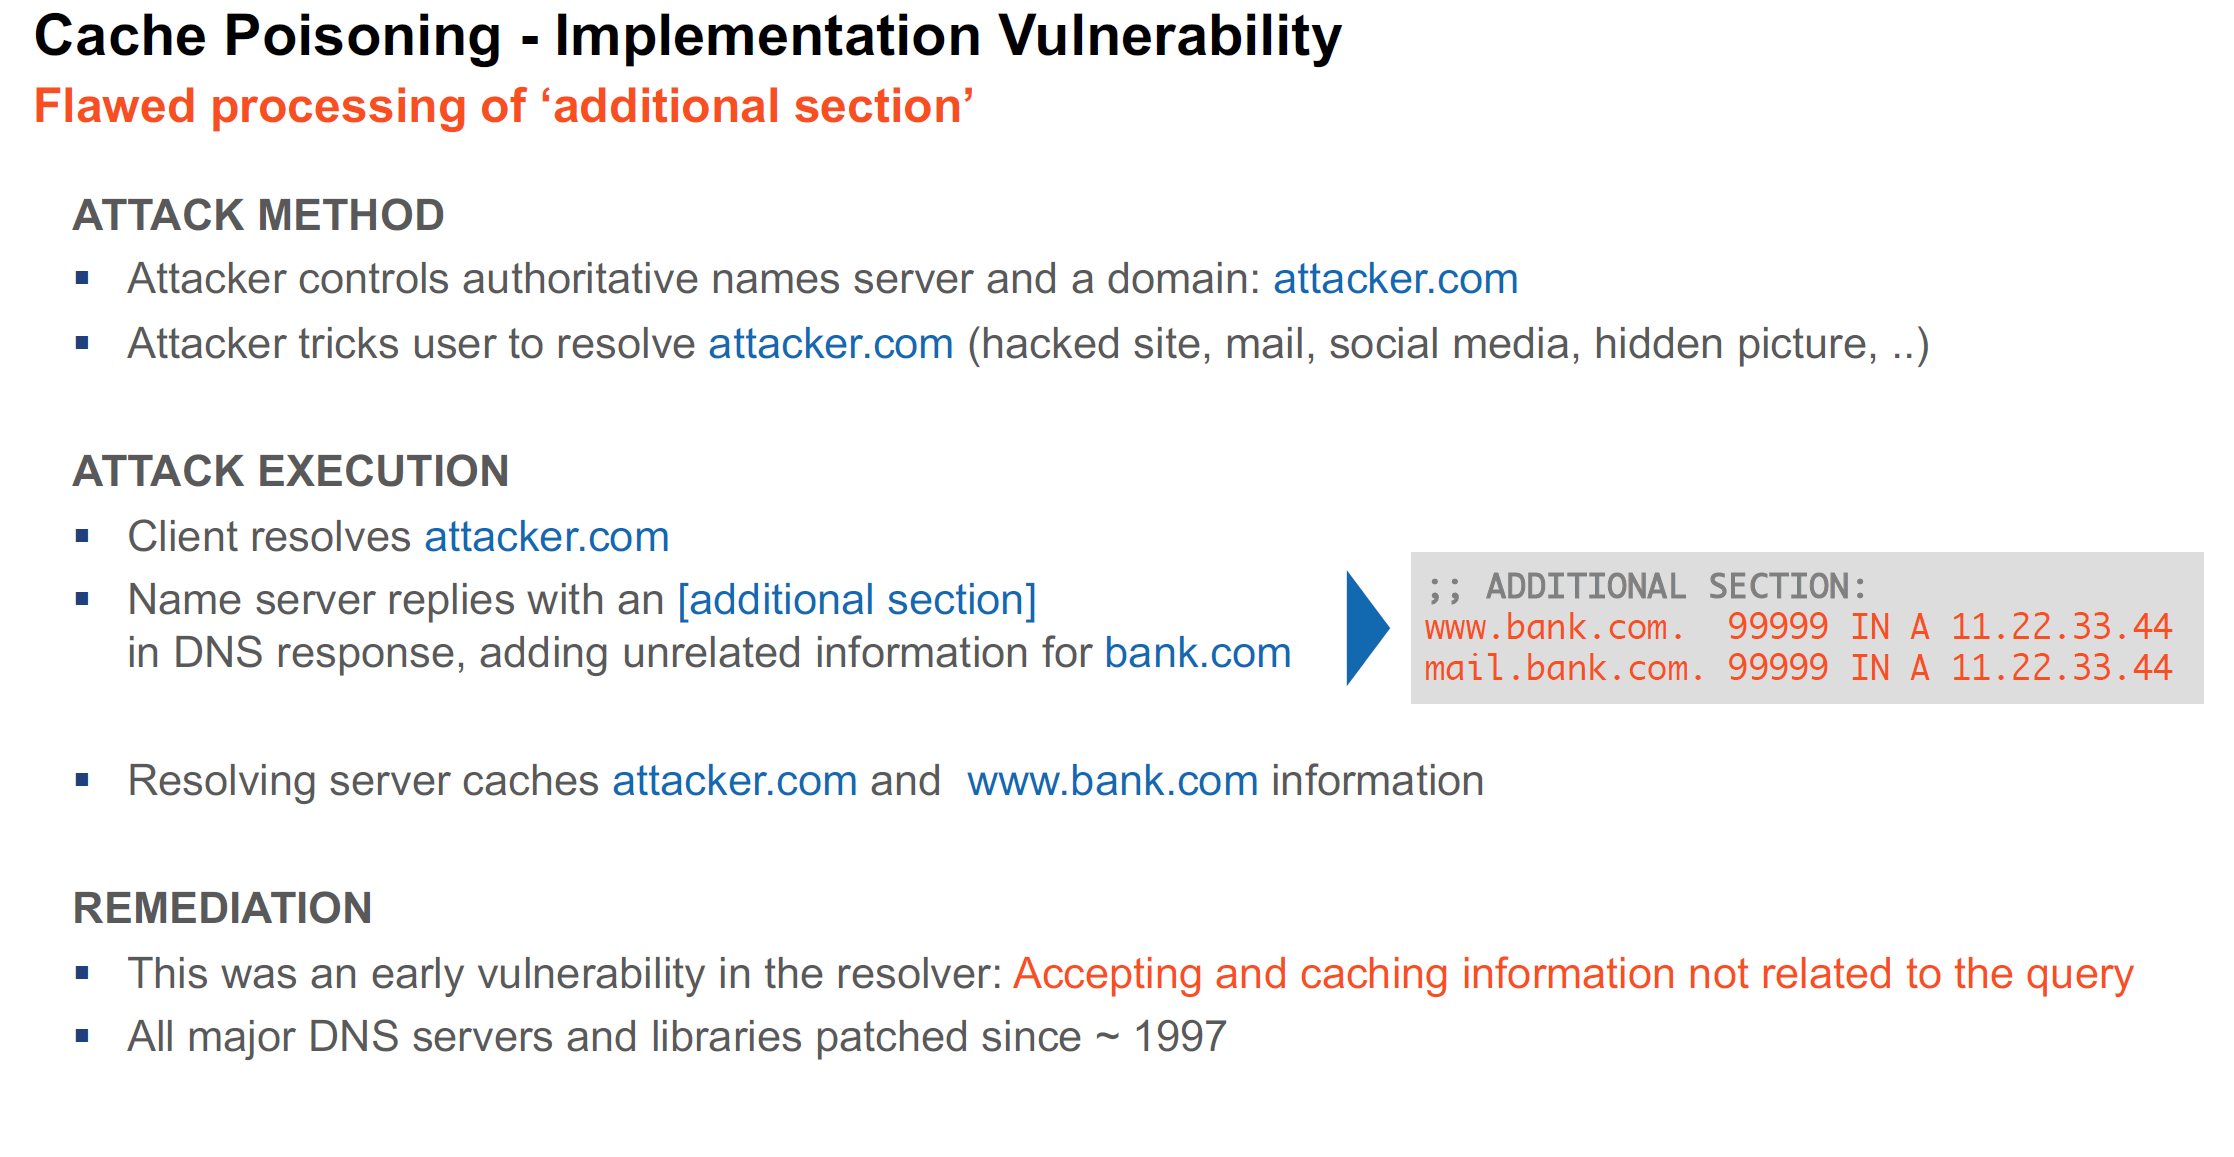
\includegraphics[width=\linewidth]{Figures/DNS_additional_section.PNG} 
\end{minipage}

\paragraph{Cache Poisoning - Guessing Game}
\begin{itemize}
    \item Attacker sends DNS query to a resolver for a nonexisting subdomain of banking.com, then sends forged response(s) as soon as the resolver queries the name server. If the injected response gets accepted the attacker has successfully injected a fake ip address for banking.com. 
    \item Only knowing the txid and source port prevent the attacker to insert his own information.
    \item At best attacker can guess: port and txid entropy (at max): $2^{16} x 2^{16} = 65'536^2$ bad odds!
    However, this is theory and we live in the real world.
    \item Attacker needs to wait until next race if his response is late or wrong - the correct info is cached until TTL expires.
\end{itemize}

\paragraph{Kaminsky Attack:} Use some tricks to make the odds turn: 
\begin{itemize}
    \item Attacker can force a server to look sth up: client-server request \& response round-trip takes time. It takes attacker no time to immediately send face response.
    \item Try lots of random txid and send a reply for each of them simultaneously.
    \item Lookup [1-100].www.bank.com -> attacker gets 100 races
    \item When found correct combination of txid and src port send additional section in reply similar to previous attack.
    \item This attack was mitigated by randomizing src port.
\end{itemize}

\paragraph{SADDNS Attack:}
\begin{itemize}
    \item When a DNS server issues a query, its source port effectively becomes open to the public.
    \item Trigger the DNS server to send a query on target server (src port becomes open to public)
    \item Mute victim Name Server to delay response (buy time for attacker)
    \item Scan port range with UDP to identify open source port.
    \item Once the source port nr is known, the attacker simply injects a large number of spoofed DNS replies bruteforcing the txid.
    \item \textbf{Mitigations:} DNSSEC, Disable ICMP port unreachable to disallow portscanning, Randomize ICMP global rate limit.
\end{itemize}

\paragraph{Learned Lessons}
\begin{itemize}
    \item Source port randomness is not everywhere truly random.
    \item Txid has insufficient randomness and entropy (only 16 bit).
    \item Birthday Paradox: Multiple outstanding requests for the same resource records.
\end{itemize}

\subsection{Compromised Configuration}

\paragraph{Attack Domain Registrar}
Top Level Domains are controlled by specific domain registrars (selected by IANA). Compromise Domain Registrar, Second level domains (SLD) are registered with one of the domain registrars of the TLD.

\begin{itemize}
    \item The DNS information is as secure as the Web App, Registration Processes, or the Passwords of the registrar and the domain owner.
    \item Hack the Web App of the domain registrar, Brute-force users password.
    \item Then change registration entries directly at the registrar. Lock owner out of his account.
\end{itemize}

\paragraph{Attack Network \& Local Configuration:} Insecure provisioning of DNS setting
Manipulate DNS configuration settings on internal network or local host. Have target point to attackers name server.
\begin{itemize}
    \item WAN Network: Scan ISP networks, identify vulnerable routers or weak/default passwords. Attack poorly protected client router of Internet Service Providers (ISP)
    \item LAN Network: Attack client router or DHCP server directly. Attack DHCP exchange in local network (Cache poisoning against DHCP: attacker replies faster than DHCP)
    \item Local Host: Manipulate DNS local hosts settings on compromised machine. Malware changes local DNS configuration (e.g. the file for static mapping of names to IPs \texttt{/etc/hosts} for linux, disable Antivirus updates by changing the mapping from download-site, or mapping of name server). Possible exploits are ad manipulation (Google ads), phishing (credit cards, online banking) or selling software (fake iTunes shops).
\end{itemize}

\paragraph{Name Server Roles}
Recursive name servers that resolve queries for anybody are a security problem:
Can be abused to launch powerful DDoS attacks from anywhere. DNS queries are typically transmitted over UDP - they are fire and forget. The source IP can be spoofed and the receiver has no way of determining its veracity before responding. The attacker will spoof the srcIP to the victim's IP - the response will thus be reflected to the victim and overload his servers. DNS also is capable of generating a much larger response than query (e.g. \texttt{dig ANY isc.org @x.x.x.x} query is 64 bytes, the response is 3,223 bytes). There are many powerful and well connected DNS servers, which can be abused to redirect large DNS responses to any target. The key to this attack are \textit{open} DNS resolvers (recursive resolver that replies to any DNS query, coming from any device
on the Internet).

\begin{itemize}
    \item Authoritative Server: responds to queries from any source. Non recursive queries. Only with data it is authoritative about.
    \item Cache/Recursive Resolver: Respond to local network only. Recursive queries. Should attempt to resolve any legitimate request
\end{itemize}

\textbf{Mitigation:} Source IP verification (reject packets with source addresses not reachable via the actual packet’s path), disable recursion on authoritative name servers, limit recursion to authorized clients, Response Rate Limiting (RRL).\\
However, the main mitigation is hosting a service on different locations in the internet, s.t. it gets harder for an attacker to target all possible locations. Using BGP anycast, the same IP address is advertised on different locations on the internet.\\
A user is directed to the nearest service location. This helps to distribute the load on different sites. There are CDN services like Akamai or CloudFlare that offer this as a service.
\\
On TCP, this attack would not work as is since the second message after the TCP SYN is not the DNS response but the TCP SYN ACK. The TCP ACK would go to the victim (due to the srcIP spoofing). The DNS response would be the second message sent by the server. However, the attacker could reply with the third handshake message + payload after intercepting the replies and dropping them. If the attacker is not Dolev-Yao, which is often the case, the attack would become tricky to perform.

\subsection{Domain Name System Security Extensions (DNSSEC)}

DNSSEC attempts to add security, while maintaining backward compatibility to the
existing DNS. DNSSEC is a set of extensions to DNS to provide resolvers:
\begin{itemize}
    \item origin authentication of DNS data
    \item authenticated denial of existence
    \item integrity
    \item But not availability or confidentiality.
\end{itemize}

\paragraph{DNSSEC Key Features:}
\begin{itemize}
    \item DNSSEC zone data is digitally signed using a private key for that zone. A DNS server receiving DNSSEC signed zone data can verify the origin and integrity of the data by checking the signature using the public key for that zone.
    \item DNSSEC can protect any data published in the DNS
\end{itemize}

\paragraph{Protection Process:} 
\begin{enumerate}
    \item Each DNS zone signs its data using a private key (recommended to do offline).
    \item A query for a particular record returns: The requested resource record set, a signature (SIG) of the requested resource record set.
    \item The resolver authenticates response using public key.
\end{enumerate}

\paragraph{DDNSSEC Resource Records:} List of added RR in dnssec

\begin{minipage}{\linewidth}
    \centering      
    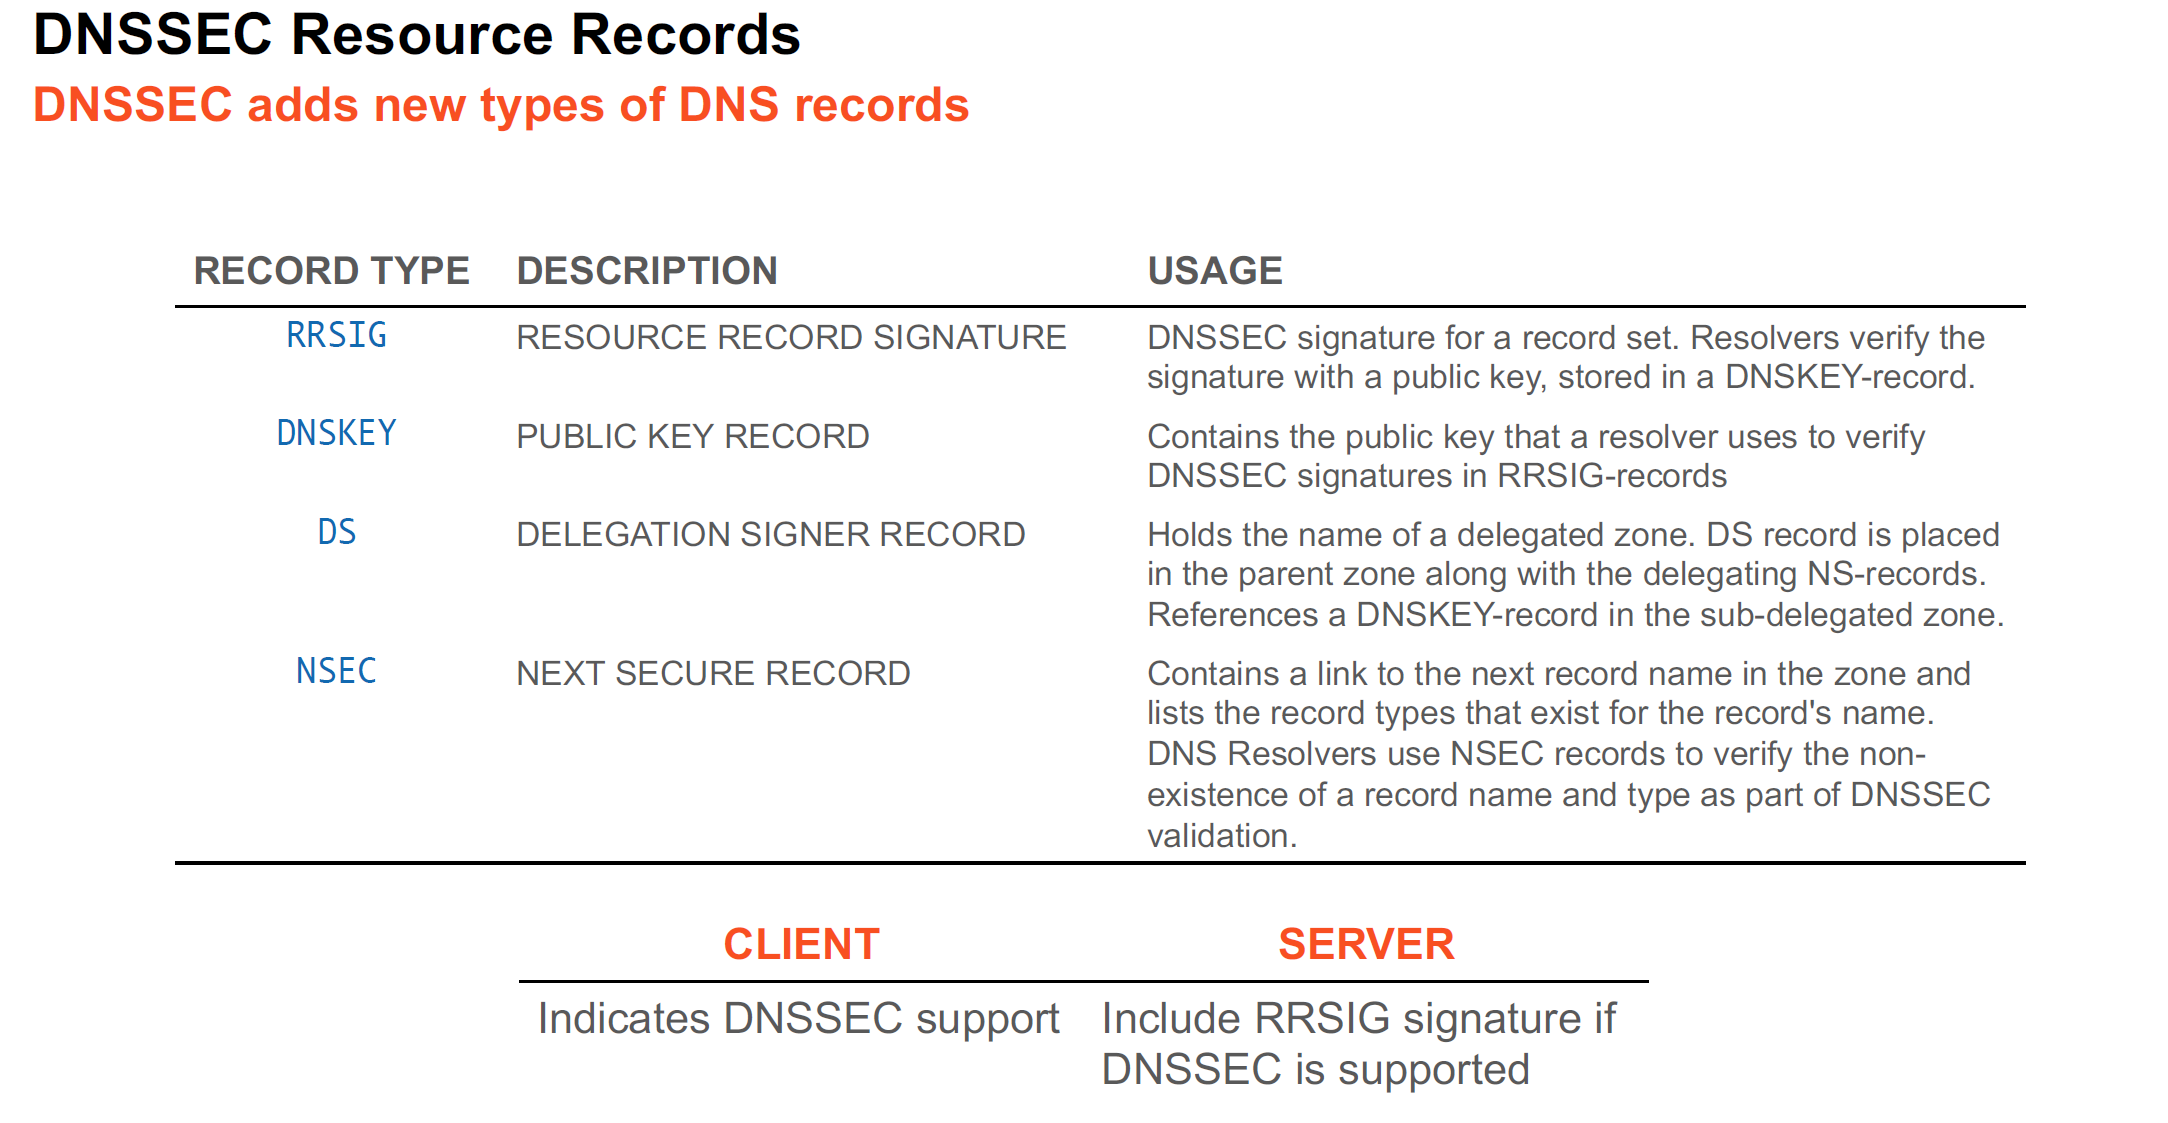
\includegraphics[width=\linewidth]{Figures/DNS_dnssec_rr.PNG} 
\end{minipage}
The DS record contains a hash of the KSK (key signing key) belonging to the
child zone. Once the DNS resolver knows the contents of DS, it can retrieve the KSK and ZSK (zone
signing key) belonging to the child zone. KSK is checked against DS. ZSK is validated using
the KSK. Finally, if the child zone is the actual target of the query, the answer
can be checked by using the ZSK.

\paragraph{DNSSEC Pros and Cons:} Advantages and disadvantages of dnssec
\begin{minipage}{\linewidth}
    \centering      
    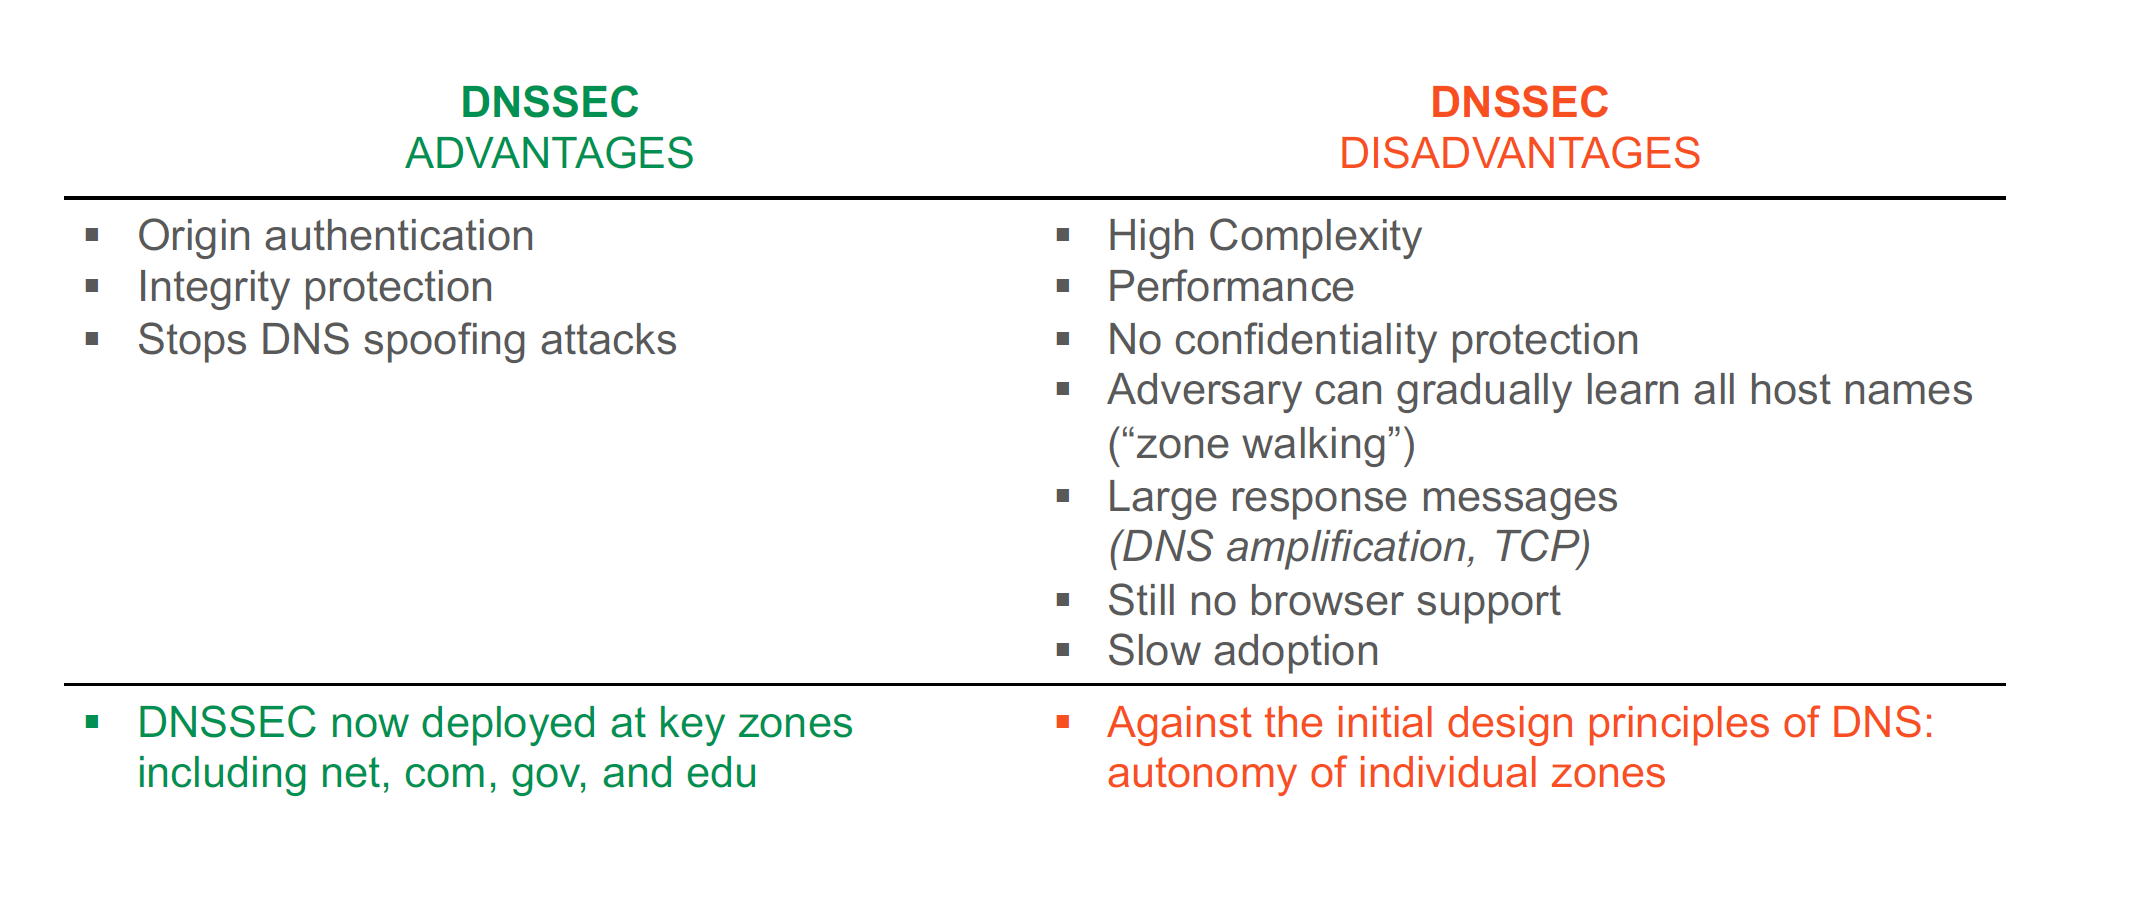
\includegraphics[width=\linewidth]{Figures/DNS_dnssec_advantages.PNG} 
\end{minipage}

\subsection{DNS over HTTPS (DoH) or TLS (DoT)}
DoT users service specific port 853, which might be filtered by firewall/attacker. DoH users standard HTTPS port (443), usually no filtering, easy integration.
Problems:
\begin{itemize}
    \item DNS messages are not protected from eavesdropping (even with DNSSEC)
    \item DNS request are an easy way of tracking users (by the ISP or intelligence services)
\end{itemize}

DOH would solve some attacks on DNS such as DNS spoofing, mass-logging of DNS requests, DNS amplification/reflection, cache poisoning, etc. However, there are disadvantages. With DOH, local caches are no longer possible – each query needs to reach the remote DoH resolver. In the case of large providers, load and latency are not a problem: anycast is used to respond to the queries in a geographically distributed way. However, this concentrates even more power in the hands of a few companies (Google, Cloudflare, etc.); the internet gets even more centralized.




\section{SCION \small (Secure Multipath Interdomain Routing Architecture)}

BGP security issues have been going on for years. Instead of trying to fix and patch BGP, why not just develop a completely new inter-AS protocol with modern requirements as features.\\

\textbf{Goals of SCION:} High availability, Secure entity authentication, Flexible trust, Transparent operation, Balanced control, Scalability, efficiency

\paragraph{SCION Architecture Principles}
\begin{itemize}
    \item Stateless packet forwarding (no inconsistent forwarding state)
    \item "Instant convergence" routing
    \item Path-aware networking
    \item Multi-path communication
    \item High security through design and formal verification (This is necessary, fromal verifications from the beginning avoids "difficult-to-verify" components
    \item Sovereignity and transparency for trust roots
\end{itemize}

\subsection{Approach for Scalability: Isolation Domain (ISD)}
The architecture of SCION mandates that the Internet is partitioned into \textit{Isolation Domains (ISDs)}, that are independently organized groupings of ASes. In each ISD, part of the ASes form the \textit{ISD core}, which is responsible for managing the whole ISD and has some special functions (e.g. Swisscom, Sunrise would be core ASes). An ISD usually represents an area of common trust or of common legislation (e.g. countries, multinational federations). ISDs are SCION's approach for scalability and they are a virtual concept: ASes can be in different ISDs and can have different roles in different ISDs.

\begin{minipage}{\linewidth}
    \centering      
    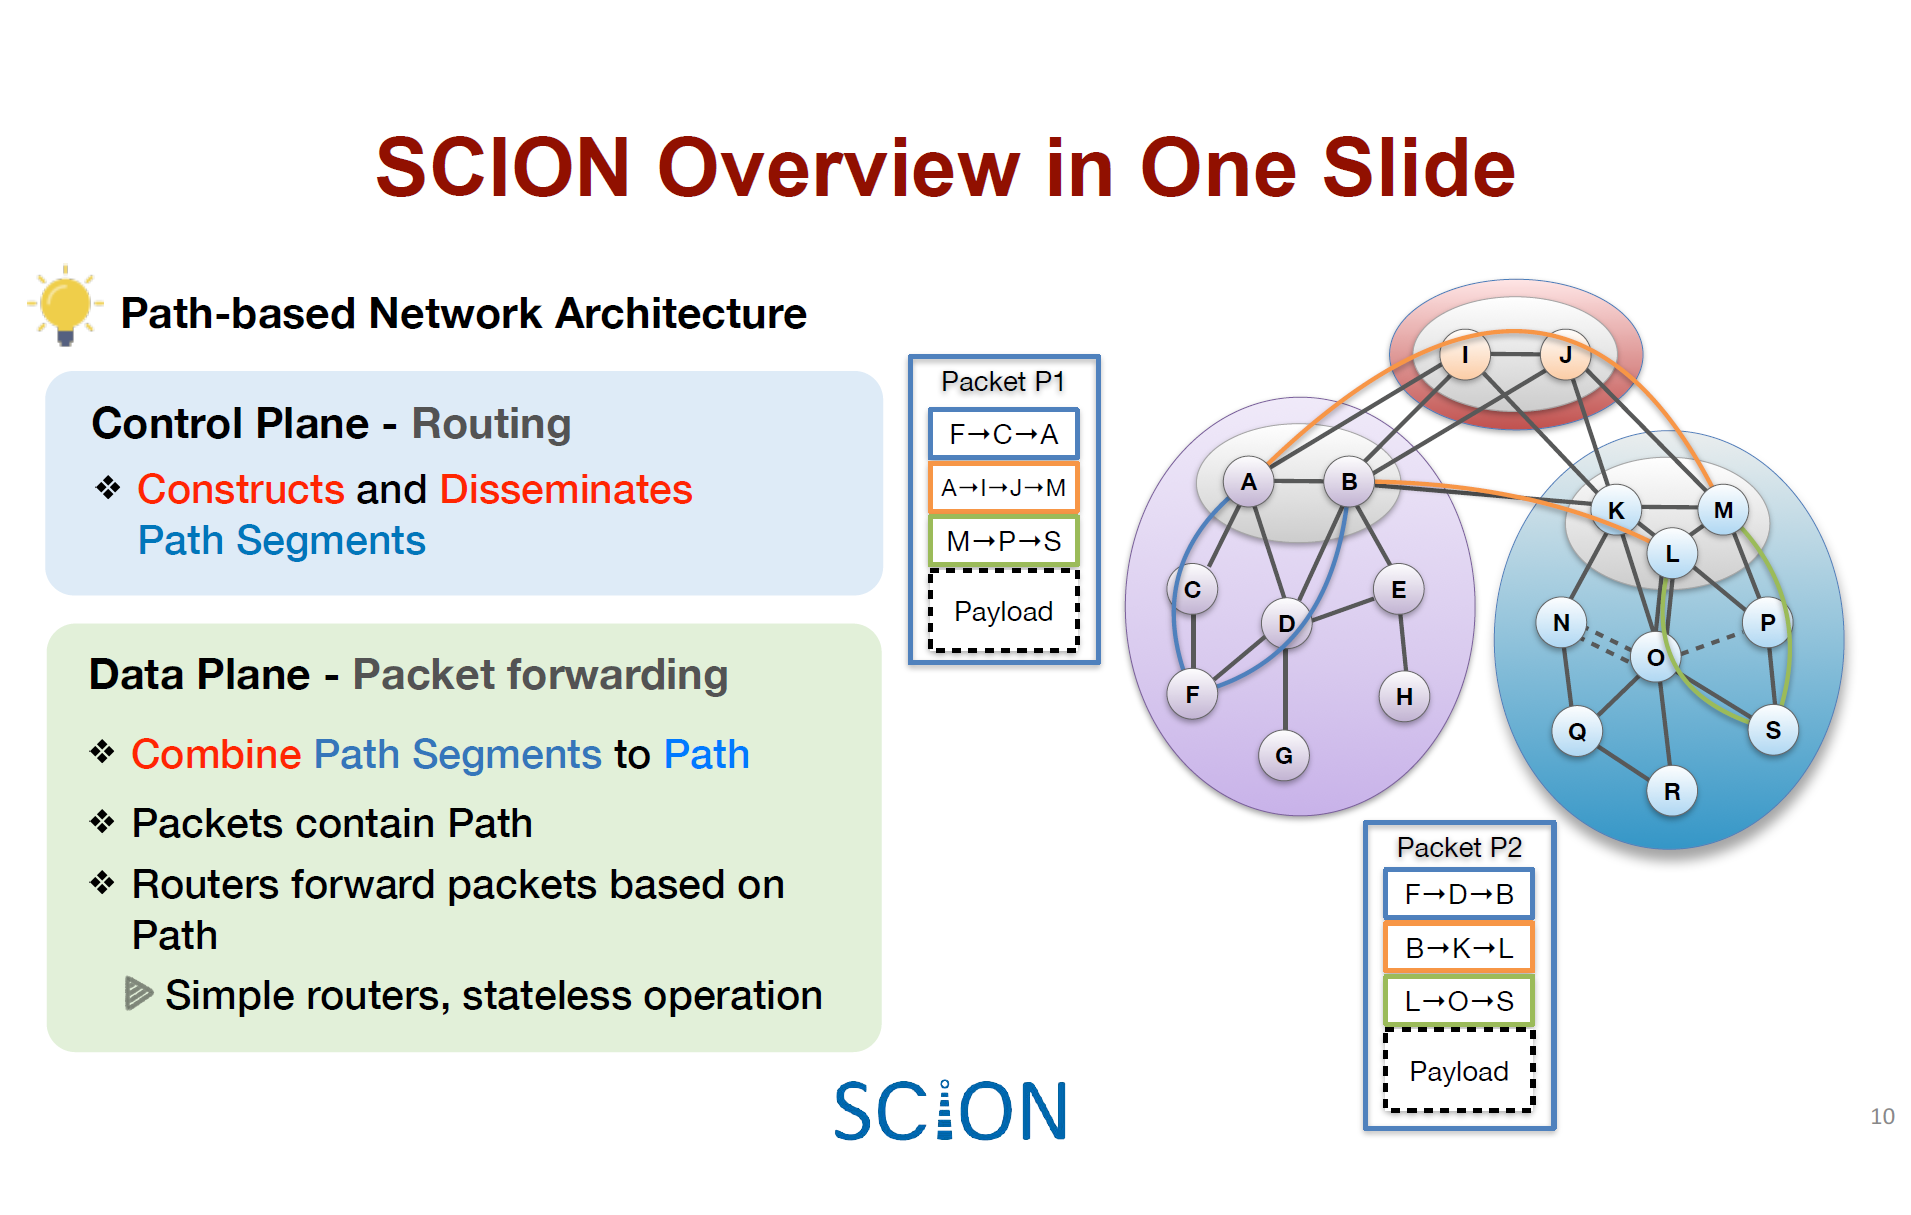
\includegraphics[width=\linewidth]{Figures/SCION_overview.PNG} 
\end{minipage}


\subsubsection{Intra-ISD Path Exploration: Beaconing}
Beaconing is am asynchronous process through which paths are found in SCION. The Core ASes in an ISD (Isolation Domain) periodically flood the ISD with PCBs, by sending them in an anycast fashion (dubbed service anycast in SCION). Any AS receiving this packet will send it to its beacon server, which will add the current AS info and send the PCB to the ASes downstream. When beacons reach leaf nodes in the AS graph, the process is completed. Each AS receives multiple PCBs representing path segments to a core AS.\\

Each AS deploys one or multiple beacon servers. SCION border routers receive PCB
and select one beacon server to forward it to. Beacon servers coordinate to resend PCBs periodically to downstream ASes (currently every 5 seconds). ASes can choose to which customers and peers to forward which beacons, but in the end it is the sources that determine the final path.\\

\textbf{PCB contents:} PCB contains an info field with: PCB creation time. Each AS on path adds: AS name, Hop field for data-plane forwarding (Link identifiers, Expiration time, Message Authentication Code (MAC)), AS signature.\\
\textit{Link identifier}: ASes have multiple interface numbers. The hop field has an \texttt{IN} and \texttt{OUT} link identifier, they say where traffic enters/ leaves the AS.\\
\textit{MAC}: highly efficient (verified in a few ns) but needs symmetric keys (only known inside the AS). This allows the AS to verify its own forwarding information.

\textbf{Up-Path and Down-Path Segments:} PCBs contain path segments that
can be used as communication paths. A path segment is any contiguous subsequence of ASes contained in a PCB, provided that at least one of the extremes is a core AS. They owe their name to the fact that they represent different segments of a whole path. Each path is comprised of an \textbf{up-path segment} (from source AS to a core AS) plus a \textbf{core-path segment} (from core AS to core AS, possibly on a different ISD), plus a \textbf{down-path segment} (from core to destination AS).\\

\subsubsection{Core Beaconing for Inter-ISD Path Exploration}
Beaconing that happens inside ISDs also happens across ISDs $\rightarrow$ core ASes beacon among each other. Beacon info looks similar as for intra ISD beaconing. With Core Beaconing for Inter-ISD Path Exploration, there is \textit{no} convergence process! Connecting the whole internet would only take a few seconds. However, finding the best and multiple paths takes longer.\\
\textit{But:} scalability of inter-ISD beaconing is actually \textbf{worse} than in BGP because we send lots of inter-ISD beacons and we also want to discover multiple paths. However, it still scales since the number of core ASes is highly limited (few tier 1 Ases).

\subsubsection{Path server infrastructure}
Every AS has its own path server. Non-core AS's path server contains up-path segments to reach the core ASes. Core AS's path server contains down-path segments and core-path segments. Caches along the way cache paths at various levels.\\
\textbf{Up-Path Segment Registration:} AS selects path segments to announce
as up-path segments for local hosts. Up-path segments are registered at local path servers.\\
\textbf{Down-Path Segment Registration:} AS selects path segments to announce as down-path segments for others to use to communicate with AS. Down-path segments are uploaded to core path server in core AS.

\subsection{Data plane: How to send packets}
In IP, the router looks up a routing table and (usually based on the destination of the packet) makes a routing decision, forwarding the packet to the appropriate interface. In SCION none of that happens: the packet already contains the forwarding information (full AS path), so a router only needs to check the next hop information in the SCION header. As a consequence, SCION packets need larger headers compared to IP.

\subsubsection{Path lookup}
Disadvantage of SCION over today's internet: we need to look up paths. In today's internet, we just lookup an IP, send a packet and pray.\\

\paragraph{Steps of a host to obtain path segments:}
\begin{enumerate}
	\item Host contacts RAINS server with a name: H $\rightarrow$ RAINS\\
	RAINS $\rightarrow$ H: ISD X, AS Y, local address Z
	\item Host contacts local path server to query path segments H $\rightarrow$→ PS: ISD X, AS Y\\
	PS $\rightarrow$ H: up-path (to local ISD core ASes), core-path (connect up-path and down-path
	segments), down-path segments (from core AS to ISD X)
	\item Host combines path segments to obtain end-to-end 	paths, which are added to packets\\
\end{enumerate}

\textbf{Path lookup: local ISD}\\
In step 2, client requests path segments from local path server. If down-path segments are not cached, local path server sends request to core path server.\\

\textbf{Path Lookup: remote ISD}\\
In step 2, client requests path segments from local path server. If down-path segments are not cached, local path server send request to core path server. If core path server does not have path segments cached, it will contact remote core path server.

Path segments are valid for several hours and cached locally. Otherwise the whole process would take too much time for each time we want to send. SCION’s path combination of up-path, core-path, and down-path segments reflect current Internet routing.\\

Problem: Economic incentives are not all prevailed in SCION: customer could choose to use a very costly link (path) since we have multiple paths available. This would be bad for the provider. \textit{But:} this could be solved by the provider by setting BW limits or just making customers pay more if they use more expensive links.

\begin{minipage}{\linewidth}
    \centering      
    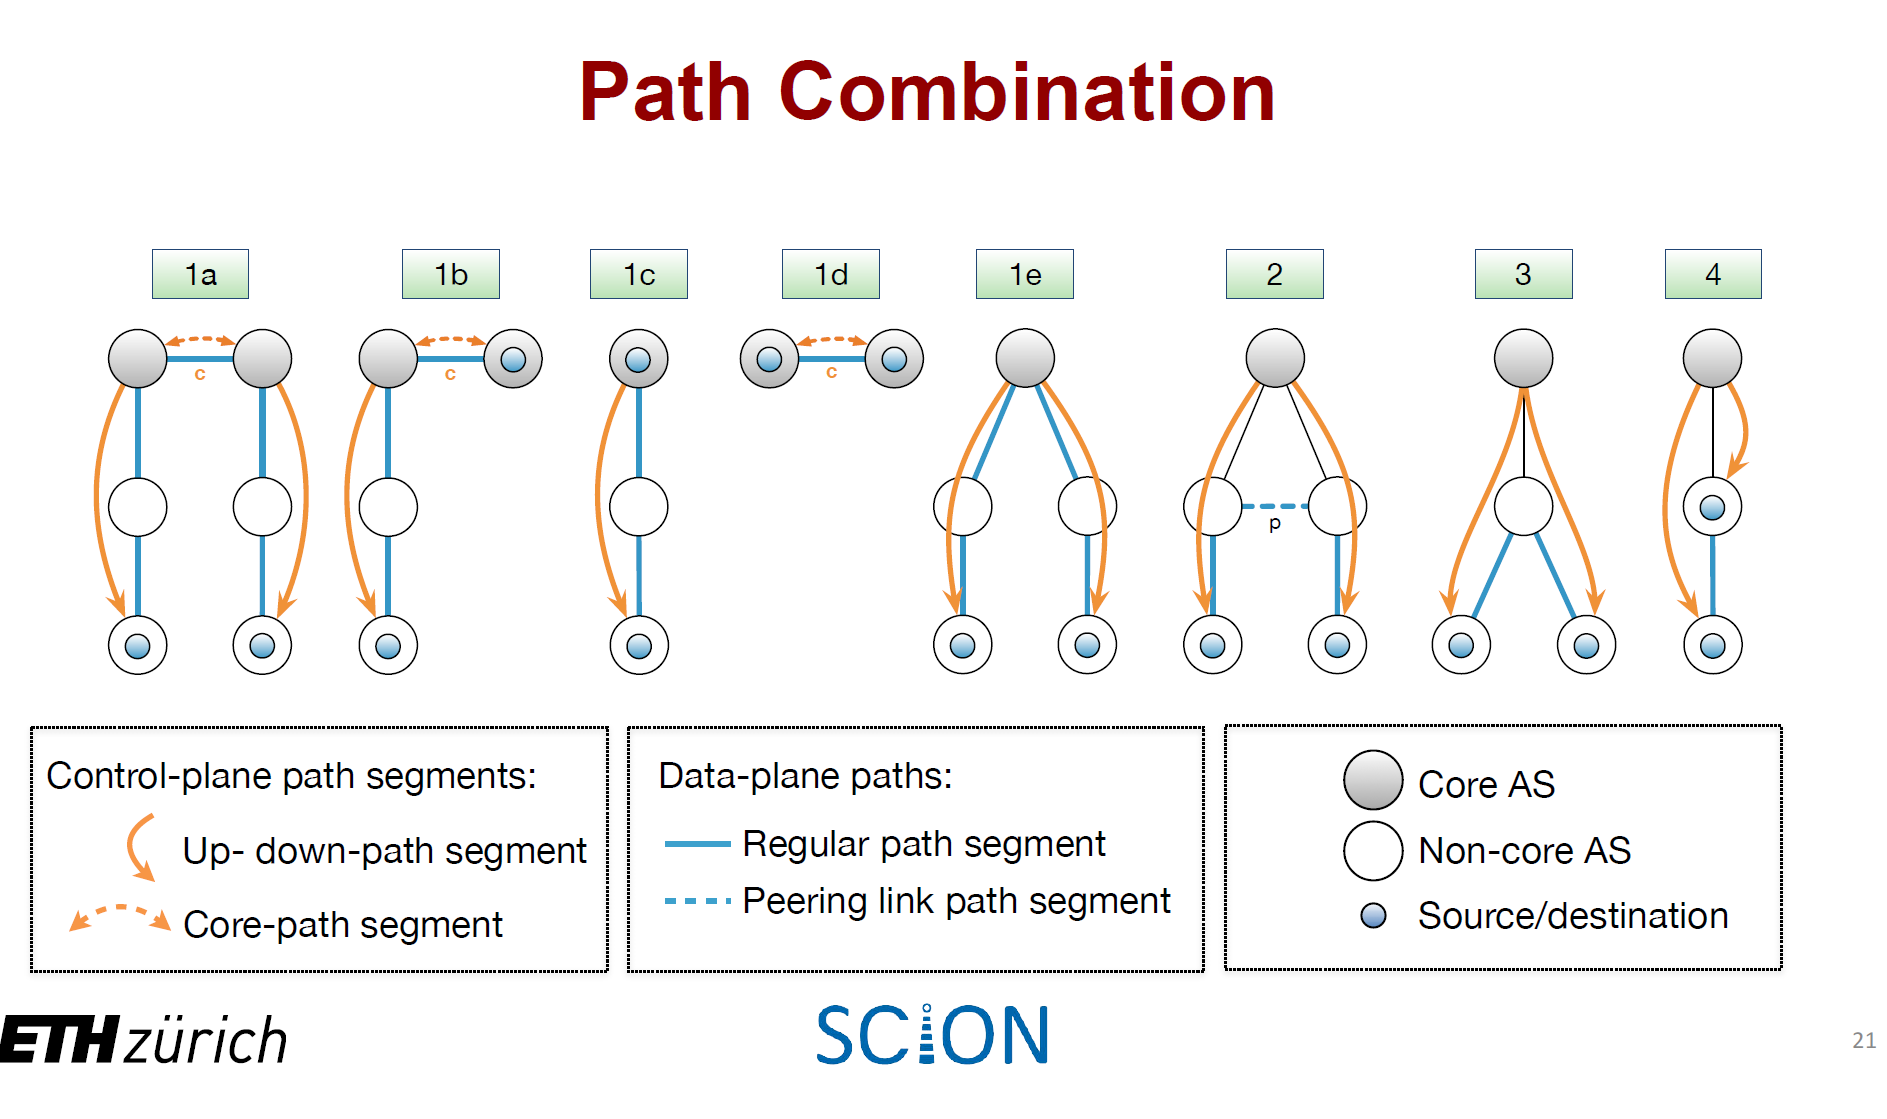
\includegraphics[width=\linewidth]{Figures/SCION_pathcombination.PNG} 
\end{minipage}

\subsubsection{SCION Packet Header}
A SCION packet has multiple headers:

\begin{itemize}
	\item SCION common header
	\item SCION source and destination address
	\item Info field provides information about a path segment
	\item Path segment consists of one or multiple hop fields
\end{itemize}

SCION does not look at srcIP \& dstIP in the network! Only when the packet gets to the destination AS will IPs be considered. \textbf{This allows for communication between private address spaces!} E.g. 192.168.0.1 in AS X could communicate with 192.168.0.1 in AS Y. Also, this would solve IPv4 address exhaustion (although IPv6 already solved it).

\begin{minipage}{\linewidth}
    \centering      
    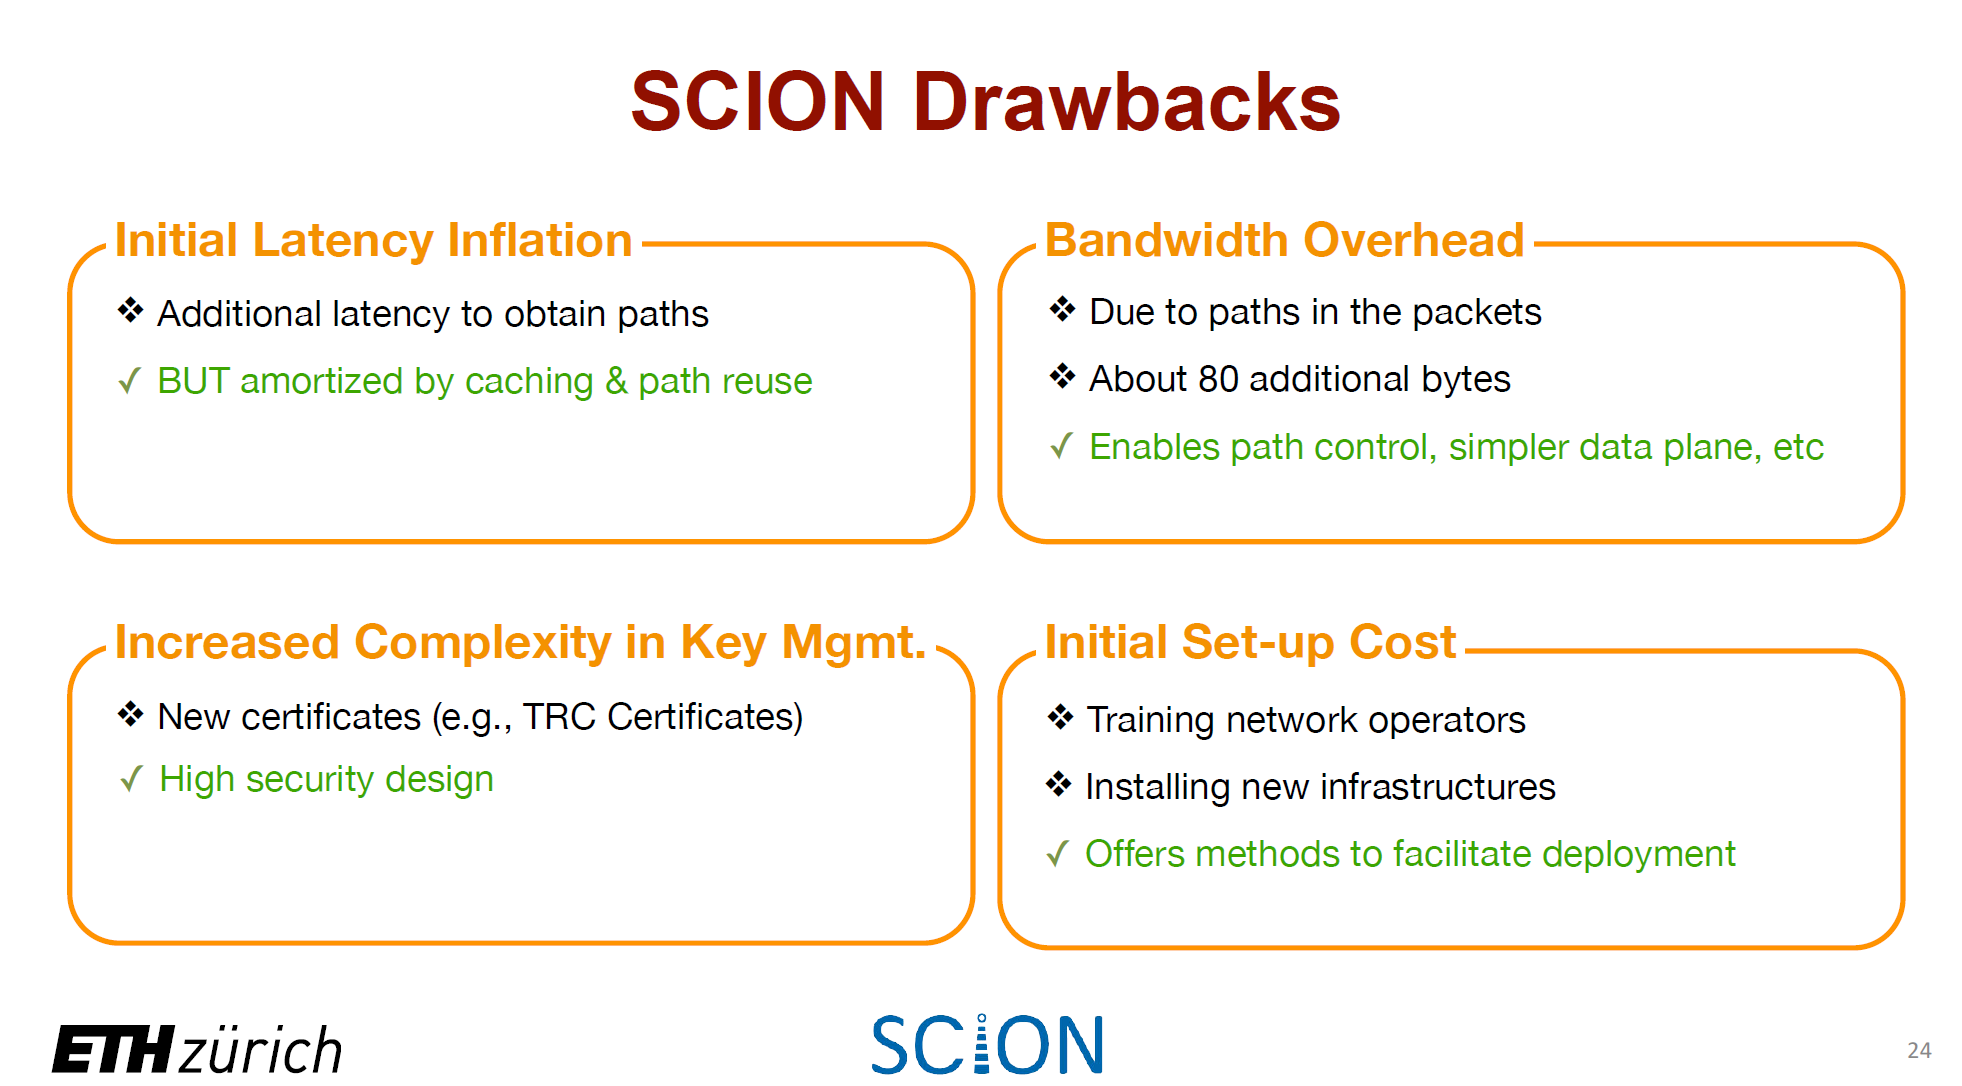
\includegraphics[width=\linewidth]{Figures/SCION_drawbacks.PNG} 
\end{minipage}

\subsubsection{Ingress and Egress Interface Identifiers}

Each AS assigns a unique integer identifier to each interface that connects to a neighboring A. The interface identifiers identify ingress/egress links for traversing AS. ASes use internal routing protocol to find route from ingress SCION border router to egress SCION border router

\subsubsection{Path Encoding in Packet}

In order to send a packet back (destination to source), we don't need to do another path lookup! The dst just needs to do some parsing to reverse the path. Forward and return paths are the same (one could also lookup a new path).

\subsubsection{Hop Field MAC Verification}

Message Authentication Code (MAC) computation and verification of Hop Field MAC value based on local AS secret key (not shared with any external entity).\\
Computation: $MAC_K(Timestamp,Flags’_{HF},ExpTime,Ingress,Egress, HF’)$, with HF the hop field of the previous AS.\\
With AESni HW crypto, only ~30 cycles are needed to compute MAC!

\subsection{Deployment and use cases}

\paragraph{ISP deployment:} Core ASes have to adapt quite a lot and need to do quite a bit of work for SCION. For regular ASes, most of this work is not needed. Integration of SCION limits to additional infrastructure such as beacon server, path server, RAINS, certificate, SIBRA and time servers.

\subsubsection{Use Case: Low-Latency Connectivity}

Generally, two paths exist between Europe and Southeast Asia: 

\begin{itemize}
	\item western route (Europe-US-SEA): High latency, high bandwidth
	\item eastern route (Europe, Suez canal, SEA): Low latency, low bandwidth
\end{itemize}

BGP is a “money routing protocol”, traffic follows cheapest path, typically highest bandwidth path. Thus, Europe-SEA traffic generally takes the western route. There is no wrong path (both have advantages and disadvantages) but the wrong thing to do is to only advertise one single path (as BGP does).

\subsubsection{Use Case: Low Earth Orbit Satellite Networks}

Speed of light in fibres is a lot slower than speed of light in free space. New Low Earth Orbit (LEO) satellite networks only require around 5ms propagation latency between earth and satellite. Inter-Satellite Laser (ISL) links enable global communication. However, LEO has frequent outages/ short time windows of availability due to changing weather conditions - BGP convergence is too slow to support. SCION however can optimally integrate LEO network into Internet fabric.

\section{Probabilistic Traffic Monitoring}

Network traffic monitoring is crucial in today's internet. Applications of traffic monitoring are broad: anomaly detection (detect DoS attack or port scans, enforce QoS), network management (accounting (often deterministic monitoring), usage-based pricing, traffic engineering). Without network management, we have no idea what's happening inside the network.\\
Large content providers such as Google, Akamai, Cloudflare constantly monitor their network to detect large traffic loads and (D)DoS attacks.\\
Why do we want probabilistic monitoring? It's more efficient.
Why do we want deterministic monitoring for accounting? Accounting happens at the edge of the network there we have enough compute power to store all states.\\

Traffic monitoring can be done at different granularities:

\begin{itemize}

	\item Per-flow basis: \textit{(srcIP, dstIP, srcPort, dstPort, protocol)}, or IPv6 flow label (20 bit)
	\item Can also monitor on a subset of the flow 5-tuple: DDos detection: \textit{(*, dstIP, *, *, *)}, source bandwidth monitoring for usage-based pricing: \textit{(srcIP, *, *, *, *)}
\end{itemize}


Traffic monitoring is difficult:

\begin{itemize}
	\item Core routers in the Internet forward multiple	terabit of traffic per second
	\item Empirical evidence: 20 million different flows on	a 1 Tbps router
	\item On a 1Tbps router we have one packet every \textit{10ns}! (1KB packets)
	\item Monitoring is especially important when something goes wrong (e.g. attacks). Exactly then it's even more challenging since we have more traffic.
	\item Attackers can craft traffic to target monitoring system (send from various ports, spoof srcIP), e.g. to exhaust state of monitoring system
\end{itemize}

\subsection{Basic Concepts of Probabilistic Traffic	Monitoring}

Intuition: trade accuracy/precision for efficiency. Deterministic monitoring is not possible for core internet. Challenge: Measure with limited memory/processing. Output an “accurate” estimate with high probability.

General concept of probabilistic monitoring: (1) Router summarizes traffic into a compact dataset. (2) Router periodically reports the dataset to a server. (3) Server estimates certain statistics based on multiple datasets.\\
(2) \& (3) are optional and not done by all systems.

\subsection{General-Purpose Measurements (NetFlow)}

Sample every packet (standard Netflow) or sample every k-th packet (sampled Netflow). Keep flow entry $\{C_{pkt}, C_{byte}\}$ for each flow, counting the number of sampled packets and bytes.\\ Estimate the number of packets and bytes with $\widetilde{n}_{pkt} = k*C_{pkt}$, $\widetilde{n}_{byte} = k*C_{byte}$.

\textbf{Advantages:} simple and efficient.\\
\textbf{Disadvantages:} Memory overhead (one entry per flow in worst case), imprecise estimate, especially for short-lived flows (we have both FP and FN), attacker could exploit by only sending large traffic in between sampling (solution: sample with probability $\frac{1}{k}$)\\

General-purpose flow measurement is either imprecise or infeasible. Solution: focus on specific traffic information (large flows, number of flows, flow distribution, ...).

\subsection{Large-Flow (Elephant) Detectors}

Large flows are flows that consume more than a given threshold of link capacity during a given measurement interval, e.g. flows that take more than 1\% of link capacity. There is evidence that less than 1\% of flows account for more than 90\% of traffic volume. It thus makes sense to look at large flows and ignore small ones.\\
It is possible to efficiently identify large flows without keeping per-flow state on routers because \#large flows $<<$ \#flows in total.

\subsubsection{Sample and Hold (Sampling based)}

This is essentially a variant of Netflow.\\
\textbf{Sample:} We sample each byte with probability p. Practically, samples a packet of size s with probability $p_s$, $p_s = 1-(1-p)^s \approx p*s$ (when p is small).\\
\textbf{Hold:} updates a flow entry for all subsequent packets once it is created. Requires flow-table lookup for every incoming packet. Flow-table stores $\{C_{pkt}, C_{byte}\}$.\\

A problem with sample-and-hold is that for large flows we need to look at all packets. Once we've seen all flows, we might need to keep track of a lot of flows.

\subsubsection{Multistage Filter (Sketch based)}

Use a CountMin sketch to estimate the number of packets of a flow.\\
\textit{Reminder}: CountMin sketches use $k$ different hash function and an array. We hash the flow-tuple with each hash function and increase all counters at the positions indicated by the hash functions. The count estimate is the minimum value of all counters.\\
\textbf{Properties}: fixed memory resources, no FNs (we can't undercount), low FPs (overcount due to hash collisions). However, we need to look at all packets, but we can keep fewer counters.

\subsubsection{EARDet Algorithm (Frequent item finding)}

\textbf{Goal}: : F ind all items that appear in a stream of m items more than k times with no false negatives\\
\textbf{Space}: n = m/k - 1 counters\\
\textbf{Algorithm:} We have $k$ counters. For each new packet $p \in f$ (flow $f$), we increase the corresponding counter for $f$ by the packet size. If no counter tracks $f$, we start tracking it. If all counters are used, we decrease \textit{all} counters by the packet size. If one counter reaches zero while decreasing, we add the current flow with the remaining packet size.\\
\textbf{Virtual traffic:} Use “virtual flows” for each idle period. Each virtual flow is at most equal to a low-bandwidth threshold ($Th_L$).\\

\textbf{Properties of EARDet:} no FN for large flows, no FP for small flows, FN \& FP possible for medium flows, deterministic (keep performance regardless of input traffic or attack pattern), relatively small storage cost (but many counters are needed)
\textbf{Disadvantage}: per-packet counter update is an expensive operation

\begin{figure}[t!]
	\centering
	\includegraphics[width=0.5\linewidth]{figures/eardet_algorithm}
	\caption{EARDet Algorithm}
	\label{fig:eardetalgorithm}
\end{figure}

EARDet is an adaption of the MG-algorithm, instead of increasing counters by number of packets, we increase counters by packet size.

\subsection{Finding Duplicates: Bloom Filters}

\textbf{Problem}: identify if an element is a duplicate\\
\textbf{Challenge}: cannot store all previous elements\\
\textbf{Solution}: Bloom filter provides probabilistic data structure for set membership testing\\

Bloom filters are a more memory-efficient approach for insertions and membership queries. Bloom filters consist of a fixed size table \texttt{bf} with $M$ 1-bit cells and $K$ hash functions and we write a 1 at each position indicate by each hash function.

\begin{figure}[hb]
	\begin{minipage}[t]{.5\textwidth} 
		\vspace{10pt} 
		\begin{itemize}
			\setlength{\itemsep}{0pt}
			\setlength{\parskip}{0pt}
			\item Insert \textit{e} into \texttt{bf}: 
			\begin{enumerate}
				\item $\forall i \in [1,K]$, calculate $h_i(e)$
				\item $\texttt{bf}[h_i(e)] = 1, \forall i \in [1,K]$
			\end{enumerate}
			\item Membership query \textit{e}:
			\begin{enumerate}
				\item if $\texttt{bf}[h_i(e)] == 1, \forall i \in [1,K]$ 
				\newline $\rightarrow$ $e$ is in \texttt{bf}
				\item else 
				\newline $\rightarrow$ $e$ is not in \texttt{bf}
			\end{enumerate}
		\end{itemize}
	\end{minipage} 
\end{figure}

\subsubsection{Dimension your bloom filter}
\label{bloom_filter_dimension}

$N$ elements, $M$ cells, $K$ hash functions, $FP$ false positive rate.

\begin{itemize}
	\item probability that one hash function returns the index of a particular cell: $\frac{1}{M}$
	\item probability that one hash function does not return the index of a particular cell: $1 - \frac{1}{M}$
	\item probability of a cell to be 0: $(1 - \frac{1}{M})^{KN}$
	\item false positive rate P(FP): $(1 - (1 - \frac{1}{M})^{KN})^K$
	\item false negative rate: 0
\end{itemize}

For an approximation, use: $p := P(FP) = (1 - (1 - \frac{1}{M})^{KN})^K \approxeq (1 - e^{-KN/M})^K$.\\

There's a global minimum when $K = \ln(2) * \frac{M}{N}  \approx 0.7*\frac{M}{N}$ found by taking derivative of $P(FP)$.\\
For that choice of $K$, resulting $p := P(FP) = 2^{-K} \approx 0.6185^{M/N}$.\\
Given optimal $K$, choice of optimal $M = -\frac{N \ln p}{(\ln2)^2}$ $\rightarrow O(N)$ space.

\textbf{In practice:} if we use the Bloom filter for a long time, it's going to fill up, which leads to more false positives (a full bloom filter we just conclude that every packet is in the filter). We thus need to reset the Bloom filter periodically. Simply resetting the whole Bloom filter leads to false negatives (all cells are back to 0 after reset).\\
In practice, we use \textit{two} same-sized Bloom filters and alternate them. We only put values into one single BF at a time and switch after a reset. \textit{BUT} for membership queries, we always check both filters! However, for very old packets we can still get FNs. Solution: use timestamps on packets and remove tracking for old packets. This gives us the FN guarantee.

\subsection{Probabilistic Counting: Estimating the Number of Flows}

\textbf{Simple probabilistic counting:} Hash flow ID to generate a value in [0,1). Keep the flow ID associated with the smallest hash value.\\
Expectation value of smallest value is 1 / (number of flows + 1).\\
Estimate the number of flows by the smallest value v seen so far: $\tilde{n} \approx 1/v - 1$.\\

\textbf{Problems:}
\begin{itemize}
	\item minimum has large variance $\rightarrow$ not very robust
	\item An attacker controlling only 1 input can bias the estimation. Solution: use private hash function or salted hashing.
\end{itemize}

\textbf{Proposal by Bar-Yossef et al. (2002):}

\begin{itemize}
	\item Keep track of the $k$ smallest hash values
	\item Expectation value of $k$-th smallest value is $k/(n+1)$, variance is smaller
	\item Estimate the number of flows by the k-th smallest value $v_k$ that has been seen
	so far: $\tilde{n} \approx k / v_k - 1$
\end{itemize}

\subsection{Traffic Monitoring vs. Intrusion Detection}

Both can detect malicious activities such as DoS attacks \& port scans at selected network
vantage points.\\
\textbf{Intrusion detection:} Typically deployed at network edges, destination-based diagnosis, can analyze detailed payload data as well.\\
\textbf{Traffic monitoring:} Can be deployed at high-speed backbone routers, diagnoses network-wide anomalies, analyzes packet headers only.


\end{multicols*}

\end{document}

